

% adapted by WS from SSR's Word document and from the 5-part series at
% https://www.overleaf.com/learn/latex/How_to_Write_a_Thesis_in_LaTeX_(Part_1):_Basic_Structure
% reviewed by MAM

\documentclass[12pt,twosided]{report}

\usepackage[titletoc]{appendix} % for adding appendix to TOC
\usepackage{biblatex}  % reference management
\usepackage{geometry}  % better margins and margin control
\usepackage{graphicx}  % to include figures
\usepackage{hyperref}  % internal and external links
\usepackage[utf8]{inputenc}  % support for non-ASCII characters
\usepackage{listings}  % typset code
\usepackage{outlines}  % easy nesting of lists
\usepackage{tabularx}  % more control over table column width
\usepackage{titlesec}  % customize chapter title 
\usepackage{upquote}  % prevent mishandling of single quotes in listings
\usepackage{float}
\usepackage{amsmath}
% \addbibresource{references.bib}


% TODO: Customize the appearance of hyperref links using \hypersetup
% See https://en.wikibooks.org/wiki/LaTeX/Hyperlinks#Customization

% Custom format of chapter title.
\titleformat{\chapter}[hang]{\bf\huge}{\thechapter.}{2pc}{}

% Separate folder for images named 'images'.
\graphicspath{ {images/} }

% Separate file for references
\addbibresource{references.bib}

% Replace with your title
\title{Rahguzar}

% Allow recalling document title
% from https://tex.stackexchange.com/a/15806/44301
\makeatletter\let\Title\@title\makeatother  

\begin{document}

\begin{titlepage}
  
  \newgeometry{top=100pt,bottom=75pt}   
  \begin{center}
    \vfill
    \textbf{\Huge \Title} \\
    {\Large \textit{Optimizing Sales with Intelligent Routing}}


    \bigskip
   
    {\large Kaavish Report\\
      presented to the academic faculty\\
      by\\\bigskip
      % replace with your name and HU ID
      \begin{tabular}{ll}
        Nabila Zahra & nz07162\\
        Rabia Shahab & rs07528\\
        Iqra Azfar & ia07614\\
        Muhammad Youshay & my07103\\
      \end{tabular}
    }\\\bigskip\bigskip\bigskip
    
\includegraphics[width=.4\textwidth]{images/HU.jpg}\\
    {\large In partial fulfillment of the requirements for\\
      \textit{Bachelor of Science}\\
      Computer Science\\\medskip
      \textbf{Dhanani School of Science and Engineering}\\\medskip
      Habib University\\\smallskip
      Spring 2025
    }\\\vfill
    Copyright {\scriptsize \textcopyright} 2024 Habib University
  \end{center}
  \restoregeometry
\end{titlepage}

%%% Local Variables:
%%% mode: latex
%%% TeX-master: "report"
%%% End:
  % title page.
\thispagestyle{empty}
\centerline{\textbf{\LARGE \Title}}
\bigskip

\vfill

This Kaavish project was supervised by:\\\bigskip\\\bigskip\\\bigskip

% TODO: Use the appropriate table below depending on whether you have an external advisor. Comment out the unused table.

% If no external supervisor.
% \hfill %
% \begin{tabular}{l}
%   \line(1,0){200}\\
%   Dr. Syeda Saleha Raza \\ % Name of your CS supervisor
%   Faculty of Computer Science\\
%   Habib University
% \end{tabular}\\\bigskip\bigskip

% % If external supervisor.
\begin{tabularx}{\linewidth}{lXl}
  \line(1,0){175} & & \line(1,0){175}\\  % Signatures.
  Fatima Alvi & & Syeda Saleha Raza \\ % Names of your supervisors
  Management Trainee & & Faculty of Computer Science\\  % External supervisor's role/job tile at their company.
  
  Salesflo Pvt Ltd & & Habib University % External supervisor's company.
\end{tabularx}\\\bigskip\bigskip

Approved by the Faculty of Computer Science on \hrulefill.

%%% Local Variables:
%%% mode: latex
%%% TeX-master: "report"
%%% End:
  % approval page.

\chapter*{Dedication}
To our parents, whose unwavering love, endless sacrifices, and heartfelt prayers have been the foundation of everything we’ve accomplished. Your belief in us, even when we doubted ourselves, gave us the strength to move forward. This journey, and all that it has brought us, is a reflection of your dedication and support.

To our families and loved ones, thank you for your patience, encouragement, and constant presence. Your understanding made room for our long hours, tight deadlines, and moments of exhaustion.

To our teachers and mentors, we are deeply grateful for your guidance and the knowledge you’ve so generously shared. Your trust in our capabilities challenged us to think bigger and work harder.

To our teammates, thank you for the long nights, the shared goals, and the spirit of collaboration that brought this project to life. Rahguzar is a product of shared vision, hard work, and mutual respect.

Above all, we dedicate this work to Allah (SWT), the source of all knowledge and strength. Without His mercy and guidance, none of this would have been possible.



\chapter*{Acknowledgements}
Alhamdulillah, all praise is due to Allah (SWT), whose endless mercy, guidance, and blessings gave us the strength and clarity to complete this project.

We are sincerely grateful to Dr. Syeda Saleha Raza, from the Faculty of Computer Science at Habib University, for her academic mentorship, thoughtful guidance, and unwavering support throughout the course of this project. Her insights and encouragement consistently pushed us to approach our work with both depth and discipline.

We also extend our heartfelt thanks to Ms. Fatima Alvi, Management Trainee at SalesFlo Pvt Ltd, for her practical guidance, domain expertise, and continuous availability. Her support helped us navigate the real-world complexities of the problem we set out to solve.

We are thankful to the Computer Science faculty at Habib University for equipping us with the knowledge and skills that formed the backbone of this project. Every course, discussion, and challenge over the past four years played a role in preparing us for this journey.

We deeply appreciate the collaboration with SalesFlo Pvt Ltd, our industry partner, for providing access to relevant datasets, business context, and timely feedback. Your involvement helped us ground our work in real operational needs.

Our gratitude also goes to the Kaavish Committee and the Office of Undergraduate Research for enabling a structured, well-supported project experience and for providing necessary resources and checkpoints along the way.

To our families and friends, thank you for your constant encouragement, patience, and understanding through all the late nights, deadlines, and moments of stress. Your support made all the difference.

Finally, we acknowledge one another. As teammates, we shared a vision, faced challenges, and built something we are proud of. Rahguzar is a result of that collective effort and commitment.



\chapter*{Abstract}
Efficient and scalable journey planning is critical for operational success in distribution and field service management. Manual and semi-automated Permanent Journey Plan (PJP) scheduling methods often lead to inefficiencies such as increased travel times, unbalanced workloads, higher operational costs, and inconsistent service quality. Rahguzar addresses these challenges through a modular, hybrid approach that automates the clustering, scheduling, and routing of field visits. The system employs a hybrid clustering strategy combining minimum spanning tree techniques with K-means refinement for effective territory segmentation, an evolutionary algorithm (EA) for generating balanced, constraint-aware weekly schedules, and Google OR-Tools Traveling Salesman Problem (TSP) solver for optimal intra-day route sequencing. Extensive experiments conducted on real-world datasets demonstrate Rahguzar’s ability to reduce travel distances, balance workloads, and maintain computational efficiency at scale. The platform's cloud-based infrastructure, dynamic adjustment capabilities, and KPI-driven monitoring further enhance its real-world applicability. Rahguzar not only automates PJP generation but also lays the groundwork for future enhancements incorporating predictive analytics, real-time dynamic routing, and broader deployment across diverse operational contexts.



% The following are automatically populated by LaTeX \chapter, \section and related, \figure, and \table.
\tableofcontents
\listoffigures
\listoftables

\chapter{Introduction}
\label{chap:intro}



\section{Problem Statement}

% In the vast fields of retail and distribution, route planning for field representatives is often done manually. This leads to multiple inefficiencies such as increased travel times, missed sales opportunities, and higher operational costs. Traditional manual route planning can be ineffective as it does not account for multiple critical variables such as traffic patterns, store service hours, and location-based priorities. This results in suboptimal routes that require more fuel consumption and increased travel costs. 

% Our proposed solution, Rahguzar, aims to address these challenges by automating route optimization using advanced algorithms, minimizing travel time, and enhancing productivity. This way, we aim to provide better and optimized routes with the potential for significant time and cost savings and a reduction in carbon footprint.

In the dynamic and ever-evolving world of retail and distribution, planning Permanent Journey Plans (PJP) plays a vital role in organizing daily route schedules for field representatives, such as sales representatives, to ensure consistent and efficient service to stores. PJPs involve determining which stores to visit on which days and assigning sales representatives while adhering to predefined constraints such as visit frequencies, even visit spacing, workload balancing, consistent assignments, holidays, and minimizing travel distances.
However, this planning process is inherently complex. Traditional manual or semi-automated approaches are unable to handle the scale and intricacies of modern Fast-Moving Consumer Goods (FMCG) operations, leading to inefficient routes that increase travel times and operational costs. Misaligned schedules result in missed visits or inconsistent service, while poor resource utilization increases inefficiencies. These inefficiencies also contribute to increased fuel consumption and carbon emissions, further escalating costs and environmental impact. Moreover, managing thousands of stores across diverse regions poses significant scalability challenges.

% There is a pressing need for a robust, intelligent system to automate PJP planning and address these challenges by ensuring optimal routes, efficient workforce utilization, and cost-effective operations while reducing the environmental footprint.

To overcome these challenges, Rahguzar is proposed as an innovative web-based solution designed to automate and optimize PJP planning, enabling efficient route generation, effective workforce utilization, and reduced operational and environmental costs.
\section{Proposed Solution}

% The proposed solution, Rahguzar, will be a web-based application that will use an algorithm to optimize routes for field representatives including but not limited to merchandisers, sales representatives, and order bookers. Our algorithm will take variables such as shift times, store profiles, service hours, store priority parameters, and historical traffic data to predict the routes and timings accordingly. This comprehensive approach ensures tailored routes for each representative, maximizing route efficiency and aligning with specific business goals. 

% The solution will provide interactive map interface where managers will have certain features available to them such as visualizing, adjusting, and scheduling visits on a daily, weekly, or monthly basis. The system’s capabilities aim to reduce travel time, operational costs, and environmental impacts.
The proposed solution, Rahguzar, is a comprehensive web-based application developed to automate and optimize the planning of PJPs for distributors, managers, and field representatives, including sales representatives, merchandisers, and order bookers, in the FMCG sector. Rahguzar generates efficient, scalable schedules that adhere to critical constraints, such as store visit frequencies, even visit spacing, workload balancing, consistent assignments, holidays, and minimizing travel distances. These tailored schedules ensure that field representatives can execute their tasks effectively while aligning with the organization’s operational goals.

The platform features a user-friendly, interactive map interface that allows managers to visualize, adjust, and schedule visits for daily, weekly, or monthly plans. Rahguzar determines the optimal number of field representatives required, improving workforce utilization and preventing inefficiencies such as overstaffing or under-hiring.

By optimizing routes, Rahguzar minimizes travel times, operational costs, and fuel consumption, significantly reducing the carbon footprint and promoting sustainability. This automation reduces the need for manual intervention, saving valuable time for managers while ensuring that field representatives have clear, efficient routes tailored to their responsibilities. Rahguzar delivers a scalable, cost-effective, and environmentally sustainable solution for modern FMCG operations, enhancing productivity, consistency, and overall service quality.
% This section gives a summary of our proposed solution, i.e. how does it solve the problem? An overview of the system is provided. A detailed description of each module of the system is presented later in Chapter ~\ref{chap:intro}.

\section{Intended User}

This section outlines the target users of Rahguzar, detailing the different types of users in the user base and their interactions with the platform.
\begin{itemize}

         \item \textbf{Managers:} Managers are the primary users of the system, responsible for creating, adjusting, and scheduling optimized journey plans for field representatives. They will interact with the platform through a user-friendly map interface to design, visualize, and modify routes. The system allows managers to generate daily, weekly, or monthly plans, adapt to specific business constraints, and ensure operational efficiency.
         \item \textbf{Field Representatives:} While field representatives, such as sales representative and order bookers, do not directly interact with the system, they are key beneficiaries of its outputs. They rely on the optimized journey plans created by managers to execute their tasks efficiently in the field, ensuring consistent and effective service to stores.

\end{itemize}


\section{Project Gantt chart and deliverables}

Deliverables for Kaavish I:
\begin{itemize}
    \item Requirements Specification Document
    \item System Architecture \& Design Diagram
    \item Prototype for Frontend and Backend Components
    \item Fully Developed Route Optimization Algorithm
    \item Performance and Evaluation Report
\end{itemize}
Deliverables for Kaavish II:
\begin{itemize}
    \item Comparison with existing Algorithms and improvements
    \item User-friendly web application with map interface
    \item Performance Metrics Dashboard
    \item Pilot Testing Framework and Results
    \item Final Project Documentation and Evaluation Report
\end{itemize}



\begin{center}
        \begin{figure}[H]
        \centering
        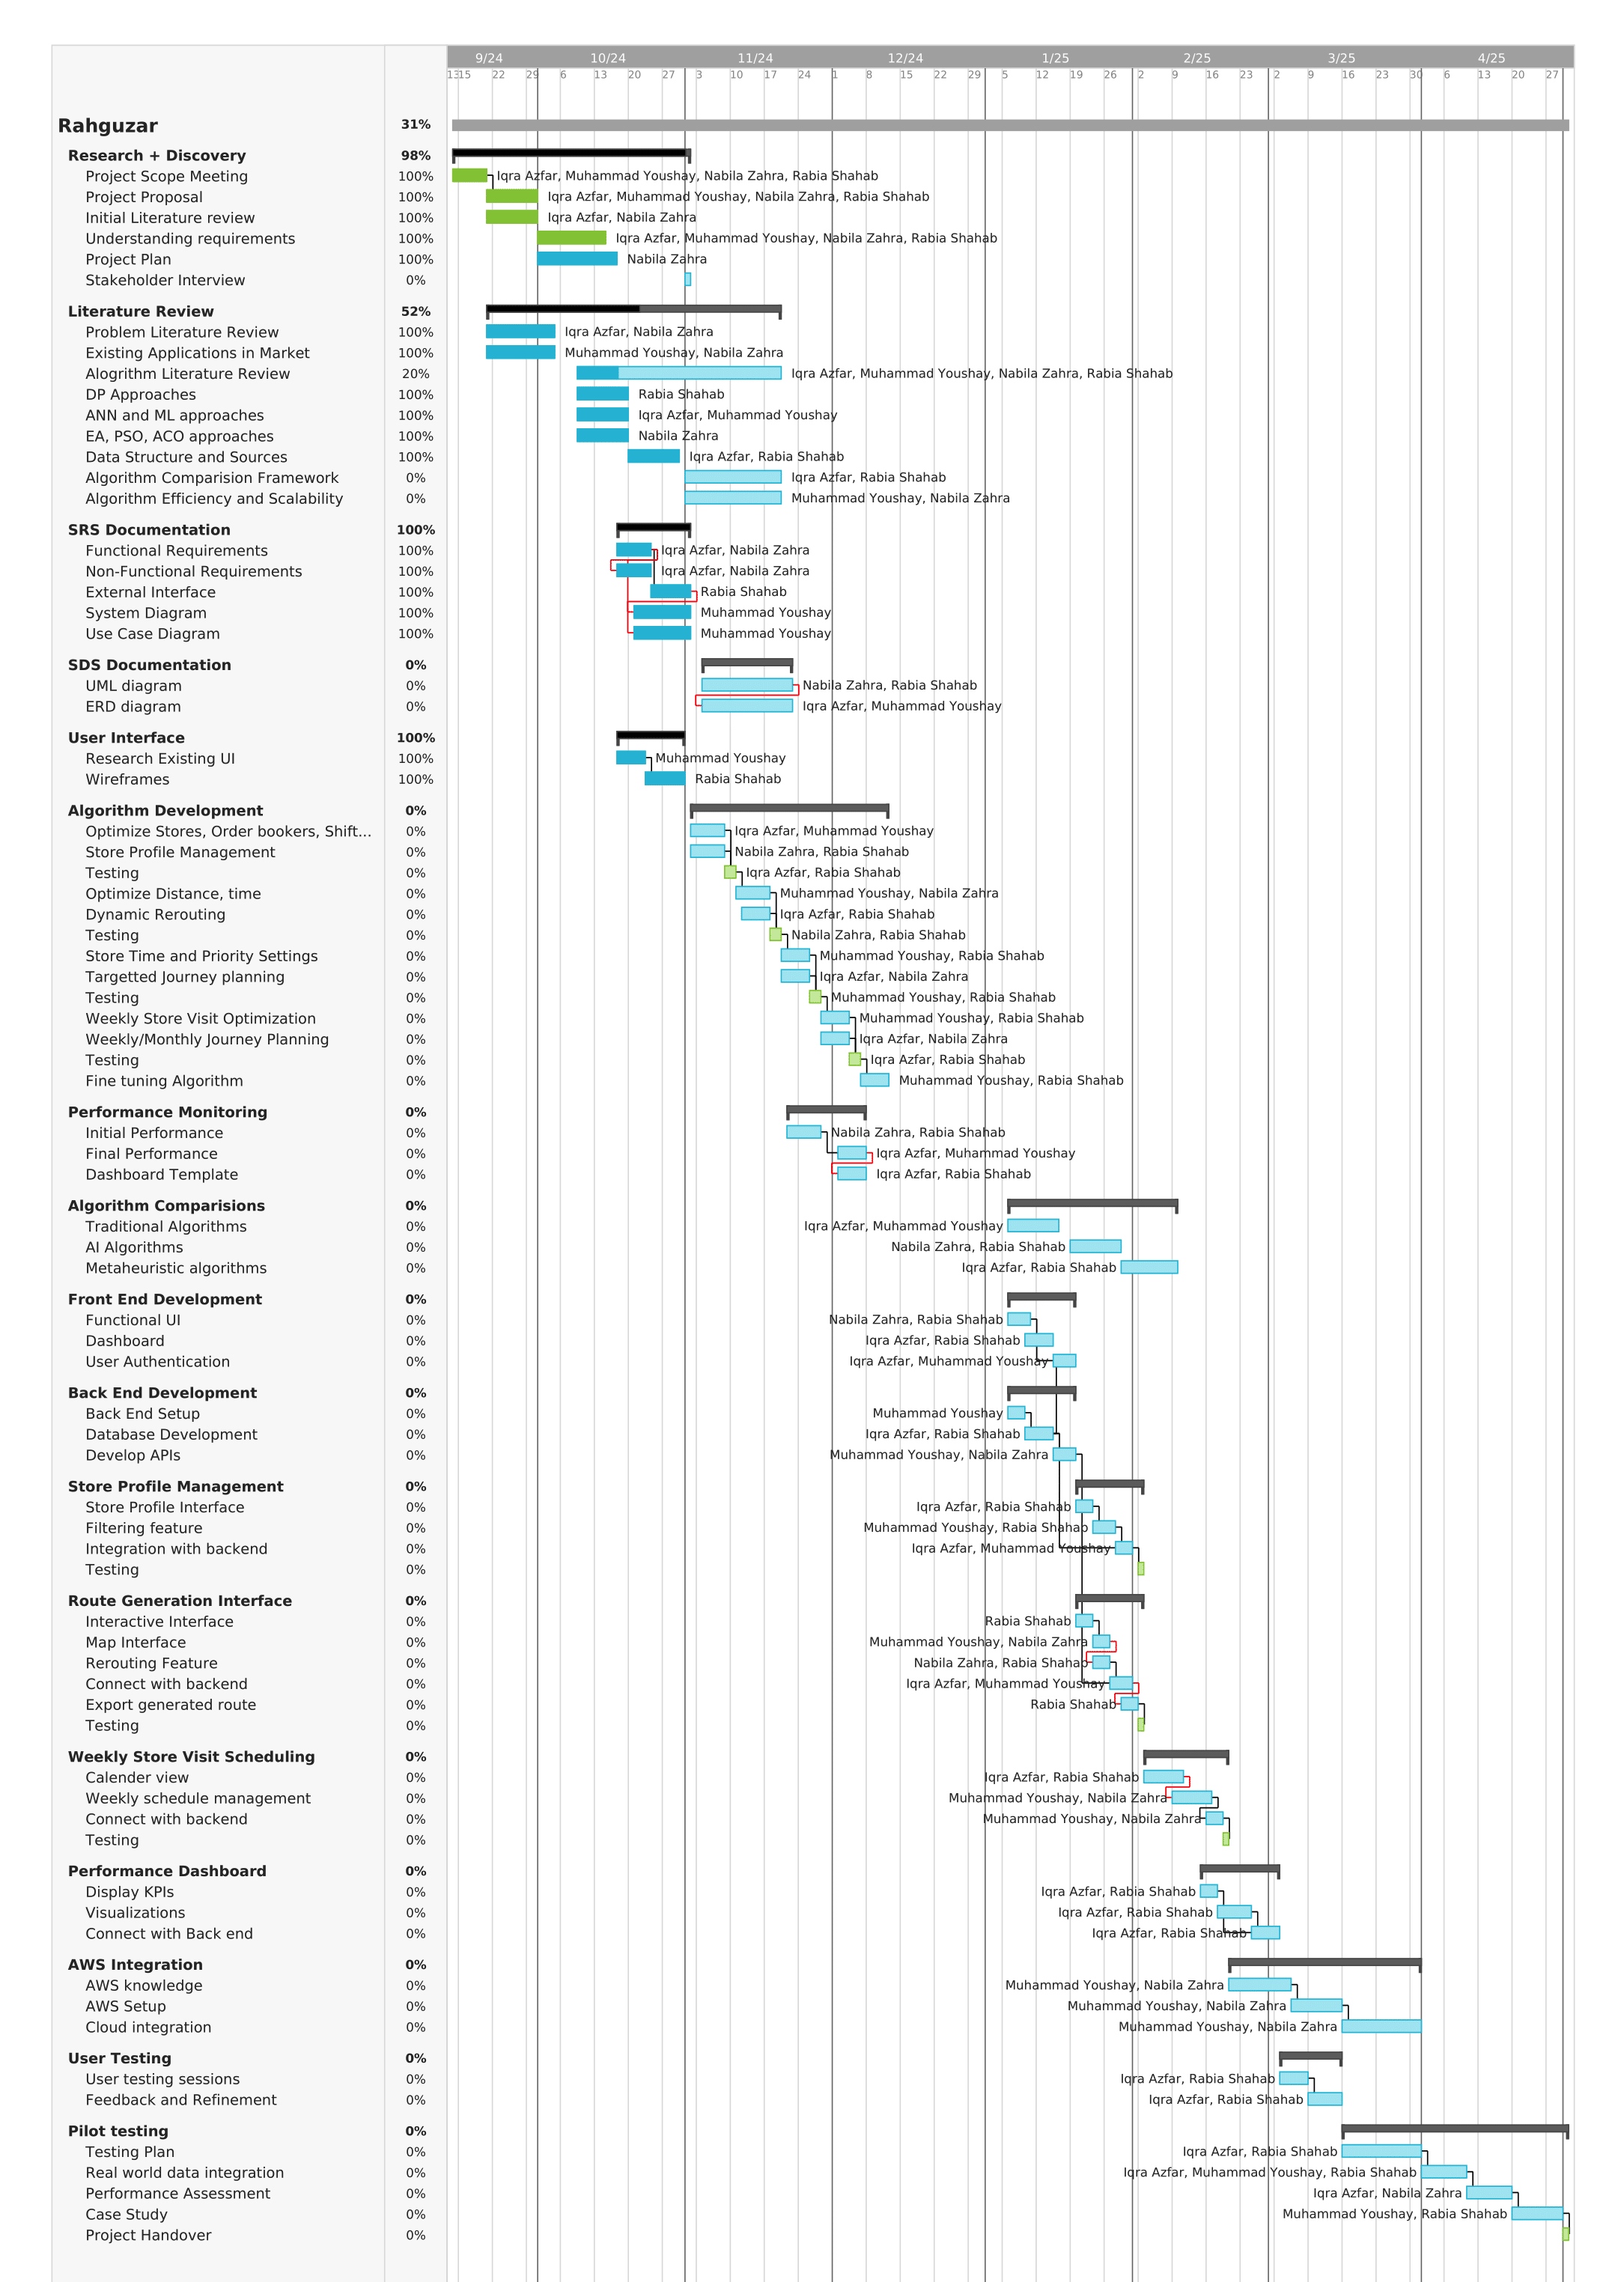
\includegraphics[width=\textwidth]{images/Rahguzar (2)-1.png} 
        \caption{Project Gantt Chart}
    \end{figure}
\end{center}

% \section{Key Challenges Encountered}

% \begin{itemize}
%     \item \textbf{Data Complexity and Integration:} Managing and integrating diverse datasets, including store profiles, geographic coordinates, and visit schedules, introduced complexity, especially when reconciling inconsistent formats and missing fields. \\
%     \textbf{Solution:} Utilize specialized data validation and transformation pipelines with Pandas and SQLAlchemy to enforce schema consistency, and incorporate early-stage data sanity checks during optimization preprocessing.

%     \item \textbf{Migration to AWS EC2:} Deploying all services (React frontend, Flask backend, Dockerized OSRM) on a single \texttt{t3.medium} EC2 instance required careful configuration of ports, firewalls, and service dependencies. Limited memory and CPU resources posed performance constraints under simultaneous loads. \\
%     \textbf{Solution:} Consolidate services through environment-based process management (e.g., Nginx + Gunicorn + Docker), configure appropriate systemd services, and optimize backend logic for memory-efficient route computation.

%     \item \textbf{Real-World Road Distance Integration:} Incorporating accurate road-based routing using OSRM required downloading and preprocessing OpenStreetMap (OSM) data, adapting coordinate formats, and ensuring routing latency was minimal in real time. \\
%     \textbf{Solution:} Host OSRM as a local Docker container within the EC2 instance, cache route queries where possible, and use GeoJSON-compatible formats to streamline frontend visualization via Leaflet.

%     \item \textbf{Frontend-Backend Route Synchronization:} Ensuring that OSRM-generated routes correctly reflected on the Leaflet map and aligned with the optimization logic was challenging, especially during cluster reassignments or manual rerouting. \\
%     \textbf{Solution:} Standardize route data in GeoJSON format across all modules and implement unified state handling in the React frontend to keep route overlays in sync with backend updates.

%     \item \textbf{Database Security and Migration:} Migrating from a local PostgreSQL database to Amazon RDS required secure credential management, reconfiguring environment variables, and restricting access through AWS security groups. \\
%     \textbf{Solution:} Use environment-based secrets management, configure RDS to allow connections only from the EC2 instance, and monitor query performance through AWS CloudWatch for optimization bottlenecks.
% \end{itemize}


\section{Key Challenges}
This section outlines the major technical and operational challenges we anticipated at the beginning of the project, along with initial strategies considered to address them. A reflection on the challenges actually encountered is presented in later chapters.


\begin{itemize}
    \item \textbf{Data Complexity and Integration:} Managing and integrating diverse datasets, including store profiles, geographic data, and workforce schedules, presents significant complexity, particularly in reconciling inconsistencies and ensuring data accuracy. \\
    \textbf{Solution:} Utilize specialized data processing libraries to streamline data handling and incorporate iterative testing phases to identify and address integration issues early in development.

    \item \textbf{Multi-Objective Optimization:} Balancing multiple optimization criteria, such as minimizing travel distances, reducing costs, meeting visit frequencies, and ensuring workload balancing, is inherently challenging due to competing priorities. \\
    \textbf{Solution:} Implement a weighted scoring system to prioritize objectives based on business needs and evaluate outputs from multiple algorithms to identify the most efficient and effective solutions.

    \item \textbf{API Costs and Performance:} Heavy reliance on mapping APIs, such as Google Maps, could lead to high costs and potentially slow performance when processing large-scale data. \\
    \textbf{Solution:} To eliminate dependency on paid APIs and ensure faster processing, we set up an Open Source Routing Machine (OSRM) server locally. This allowed us to perform routing and distance matrix calculations at scale, completely free of cost.    

    \item \textbf{Adaptability to Business-Specific Constraints:} Organizations may have unique and variable constraints, such as holidays, visit frequency, or workload preferences, which require flexible accommodation in the route planning system. \\
    \textbf{Solution:} Design the system to allow customization of route parameters and enable managers to manually adjust routes through an intuitive interface, ensuring flexibility for diverse business requirements.
  % \item \textbf{Data Complexity and Integration:} Integrating diverse datasets such as store profiles and geographic data, is complex and requires rigorous data reconciliation. \\
    % \textbf{Solution:} Use specialized libraries to streamline data handling and implement iterative testing phases to identify integration issues early.

    % \item \textbf{Multi-Objective Optimization:} Balancing multiple route optimization criteria (time, cost, distance, etc.) is challenging. \\
    % \textbf{Solution:} Apply a weighted scoring system to prioritize objectives and compare outputs from different algorithms to determine efficiency among them.

    % \item \textbf{API Costs and Performance:} Heavy reliance on Google Maps API may incur costs and slow performance. \\
    % \textbf{Solution:} Implement efficient API usage practices, such as batch processing, to minimize calls and costs. Moreover, we aim to utilize the trial phases of these services to implement them in our project. 

    % \item \textbf{Adaptability for Business-Specific Constraints:} Organizations may have unique, varying constraints that the model needs to accommodate flexibly. \\
    % \textbf{Solution:} Allow customization of route parameters and provide managers with control to manually adjust routes based on specific business needs.
    
\end{itemize}

\chapter{Literature Review}
\label{chap:lit}
This chapter presents the current state of the art in the domain and talks about other similar work that has been done in this area. It also establishes the novelty of our work by highlighting the differences between the existing work and our work.

We will keep updating this chapter (especially if our project is research-intensive) as our research proceeds and we come across more work related to our problem.

Of course, we take inspiration from \cite{einstein} but wish the work was typeset in \LaTeX \cite{knuthwebsite}, e.g. by taking help from \cite{latexcompanion}.

\chapter{Software Requirement Specification (SRS)}
\label{chap:srs}
This Software Requirements Specification (SRS) outlines the software and system requirements for Rahguzar, a route optimization project aimed at improving efficiency in retail and distribution. It details functional requirements for system capabilities and non-functional requirements like performance and scalability. The document also includes system block diagrams, use cases, and external interfaces to clarify the system’s design and interactions.

\section{Functional Requirements}


% This section describes each function/feature provided by our system. These functions are logically grouped into modules based on their purpose/users/mode of operations etc (as per our system). A functional hierarchy may look like:

The functional requirements for this system focus on creating an efficient journey-planning solution tailored for order bookers and sales representatives. This system is designed to optimize routes based on key operational parameters and provide dynamic rerouting, while also supporting targeted store visits and frequency schedules. Additional modules include a user-friendly web platform, pilot testing and validation, and performance monitoring to ensure enhanced efficiency and measurable sales impact.The following are the functional requirements for each module and their respective functions.

\subsection*{Module 1: Route Optimization Algorithm}
\subsubsection*{Function 1: Route Generation}
\begin{itemize}
    \item Implement an algorithm that creates journey plans optimized for order bookers and sales representatives.
    \item The optimization should consider multiple factors:
    \begin{itemize}
        \item[] \textbf{Sub Function 1: Order Booker Shift Times} \\
            Align route planning with the working hours of each order booker.
        \item[] \textbf{Sub Function 2: Number of Shops to Visit} \\
            Adjust routes to maximize the number of shops visited within constraints.
        \item[] \textbf{Sub Function 3: Number of Order Bookers Available} \\
            Allocate routes based on the number of available staff.
        \item[] \textbf{Sub Function 4: Total Distance Traveled} \\
            Minimize the total distance covered during journeys.
        \item[] \textbf{Sub Function 5: Total Travel Time} \\
            Reduce the time taken to complete the planned routes.
        \item[] \textbf{Sub Function 6: Store Service Times} \\
            Account for different service time requirements at each store.
    \end{itemize}
\end{itemize}

\subsubsection*{Function 2: Dynamic Rerouting}

    % \item Integrate a feature to adjust routes based on updated data (e.g., traffic, store closure).
    % \item The rerouting should optimize new paths instantly to maintain efficiency.

    \begin{itemize}
        \item It allows users to adjust the generated routes based on their preferences. They can move stores between order bookers and modify store status (e.g., active/inactive).
        \item It simply enables real-time rerouting, with the algorithm instantly updating the allocation of stores and route paths to reflect user preferences, providing flexibility and adaptability in journey planning.
    \end{itemize}

 

% \subsection*{Module 2: Weekly Store Visit Optimization 
% }

\subsubsection*{Function 3: Store Visit Frequency: 
}

\begin{itemize}
    \item Design the algorithm to include visit frequency for each store (e.g., once, twice a week).
    \item Ensure that the routes align with required visit frequencies without any overlap and maintains at least a 3 day gaps between repeated visits.
\end{itemize}

\subsubsection*{Function 4: Journey Planning for Different Timeframes: 
}

\begin{itemize}
    \item Support the generation of routes 
by allowing custom day plan creation and enable downloads for extended periods, based on the target timeframe.
    \item Ensure that stores are scheduled accurately according to their frequency needs while minimizing travel and maximizing coverage.
\end{itemize}



 

% \subsection*{Module 3: Store Profile Management and Integration }

\subsubsection*{Function 5: Store Profiling: }

\begin{itemize}
    \item Maintain detailed profiles for each store, including:
    \begin{itemize}
        \item[] \textbf{Sub Function 1:} Geographical hierarchy (region, zone, territory, town).
        \item[] \textbf{Sub Function 2:} Sales channel type (e.g., wholesale or retail).
    \end{itemize}
    \item Enable users to filter stores by parameters like region, sales channel, or visit frequency. Allow custom filters linked to all stores by uploading relevant data (e.g., location, sales volume), enabling dynamic application across stores. This approach enhances flexibility and control in route optimization.
    \item Enable users to modify store status (active/inactive) directly within the system.
\end{itemize}

\subsubsection*{Function 6: Targeted Journey Plans:}
 
\begin{itemize}
    \item Enable the system to generate routes targeting specific store types (e.g., only wholesale stores in a particular region).
    \item Allow users to select areas and stores for targeted visits, ensuring that the algorithm generates routes based on these selections.
\end{itemize}

 

\subsection*{Module 2: Web Application Platform 
}

\subsubsection*{Function 1: User Interface for Route Management: 
}

\begin{itemize}
    \item Create a user-friendly web interface for managers to access and manage journey plans.
\end{itemize}
\subsubsection*{Function 2: Integrate Map Interface:
}

    \begin{itemize}
        \item Designing, viewing, and adjusting routes.
        \item Displaying essential shop details (e.g., store profiles, geographical location).
        \item Defining and viewing boundaries like regions, territories, and areas.
    \end{itemize}

\subsubsection*{Function 3: Manual Override and Adjustment: 
}

\begin{itemize}
    \item Provide a manual override feature that allows managers to adjust routes manually.
    \item Include input options for master data (store profiles, visit frequencies, geographical details) directly within the platform.
\end{itemize}

\subsubsection*{Function 4: Downloadable Reports: 
}

\begin{itemize}
    \item Allow users to export optimized or manually adjusted routes in a downloadable format for offline analysis or distribution.
\end{itemize}

\subsection*{Module 3: Pilot Testing and Validation }

\subsubsection*{Function 1: Test Plan Creation: 
}

\begin{itemize}
    \item Develop a comprehensive pilot testing framework to validate the system's effectiveness.
\end{itemize}
\subsubsection*{Function 2: Real-World Data Integration: }

\begin{itemize}
    \item Gather real-world data during pilot testing, ensuring data is accurate and reliable.
\end{itemize}

\subsubsection*{Function 3: Performance Assessment: }
\begin{itemize}
    \item Collect and analyze data (travel time, number of shops visited, sales impact, etc.) to assess system performance.
    \item Implement an adjustment process based on pilot feedback to enhance the algorithm.
\end{itemize}

\subsubsection*{Function 4: Case Study Development: }

\begin{itemize}
    \item Compile a case study summarizing the outcomes, findings, and system performance.
\end{itemize}

\subsection*{Module 4: Performance Monitoring and Reporting }

\subsubsection*{Function 1: Key Performance Indicators (KPIs): }

\begin{itemize}
    \item Track and display metrics like:
\end{itemize}
    \begin{itemize}
    \item[] \textbf{Sub Function 1:} Average travel time per route.
    \item[] \textbf{Sub Function 2:} Number of shops visited per shift.
    \item[] \textbf{Sub Function 3:} Number of order bookers required per distribution.
    \item[] \textbf{Sub Function 4:} Sales uplift due to route optimization.
    \item[] \textbf{Sub Function 5:} Algorithm response time for route recalculations.
\end{itemize}
 

\subsubsection*{Function 3: Metrics Dashboard:
}

\begin{itemize}
    \item Develop a dashboard to visualize KPIs, providing insights into efficiency improvements, time savings, and sales increases.
\end{itemize}




% --- The above is to be modified as per your project, e.g. a flat list if your system has limited functional requirements.

\section{Non-functional Requirements}

% This sections mentions the specific non-functional requirements of our system. These generally address performance, scalability, safety, availability, deployment etc.

The Non-functional requirements define the quality and performance attributes of this system, focusing on scalability, usability, and reliability. They ensure optimal performance under varying conditions while maintaining data security and adaptability for user needs. Additionally, following requirements also facilitate maintainability for future enhancements, ensuring the system remains effective over time.



\begin{enumerate}
    \item \textbf{Scalability, Efficiency, and Memory Optimization}
    \begin{itemize}
        \item The system is designed to efficiently handle large datasets and scale up to 1000+ stores effectively as the amount of data increases, ensuring optimal performance and quick response times within 2 minutes for route generation.
        \item It should also have a low memory footprint, ensuring that it can scale effectively without degrading system performance or requiring excessive computational resources.
    \end{itemize}
    
    \item \textbf{Usability}
    \begin{itemize}
        \item A user-friendly web application interface is required, allowing users to manage, optimize, and adjust journey plans easily.
        \item The map interface must provide intuitive visualization and interactivity for planning and real-time adjustments.
    \end{itemize}
    
    \item \textbf{Reliability and Performance}
    \begin{itemize}
        \item The optimization algorithm should be robust, quickly generating optimal routes based on parameter changes, such as order booker shifts or the number of stores per booker.
        \item The system should maintain a minimum uptime of 95\%, allowing for up to 36 hours of downtime per month for a smooth user experience.
        
    \end{itemize}
    
    \item \textbf{Security}
    \begin{itemize}
        \item Data security protocols should protect sensitive information such as store profiles and geographical hierarchies, especially when integrating third-party APIs.
        \item User authentication mechanisms should be implemented to ensure that only authorized personnel can access sensitive data and functionalities within the system.

    \end{itemize}
    
    \item \textbf{Adaptability and Flexibility}
    \begin{itemize}
        \item Manual override functionality should allow users to adjust routes when needed, ensuring flexibility in route planning.
        \item The system should support long-term planning options, including daily, weekly, or monthly route generation and optimization.
    \end{itemize}
    
    \item \textbf{Maintainability}
    \begin{itemize}
        \item The architecture should allow for future enhancements, such as integrating additional parameters or algorithms for optimization, without significant rework.
    \end{itemize}
    
\end{enumerate}

\section{External Interfaces}

% We expect every project to have at least of the following subsections. This section must be aligned with your project deliverables. Please consult with your project supervisor regarding which of the following section(s) you should include in your report

\subsection{User Interfaces}
The Web application interface is designed to be user-friendly and intuitive, allowing managers to easily navigate through the system. The interface includes various features such as route management, store profiling, and performance monitoring. The design focuses on providing a seamless experience for users, enabling them to efficiently manage their journey plans and access relevant data.

\begin{figure}[H]
    \centering
    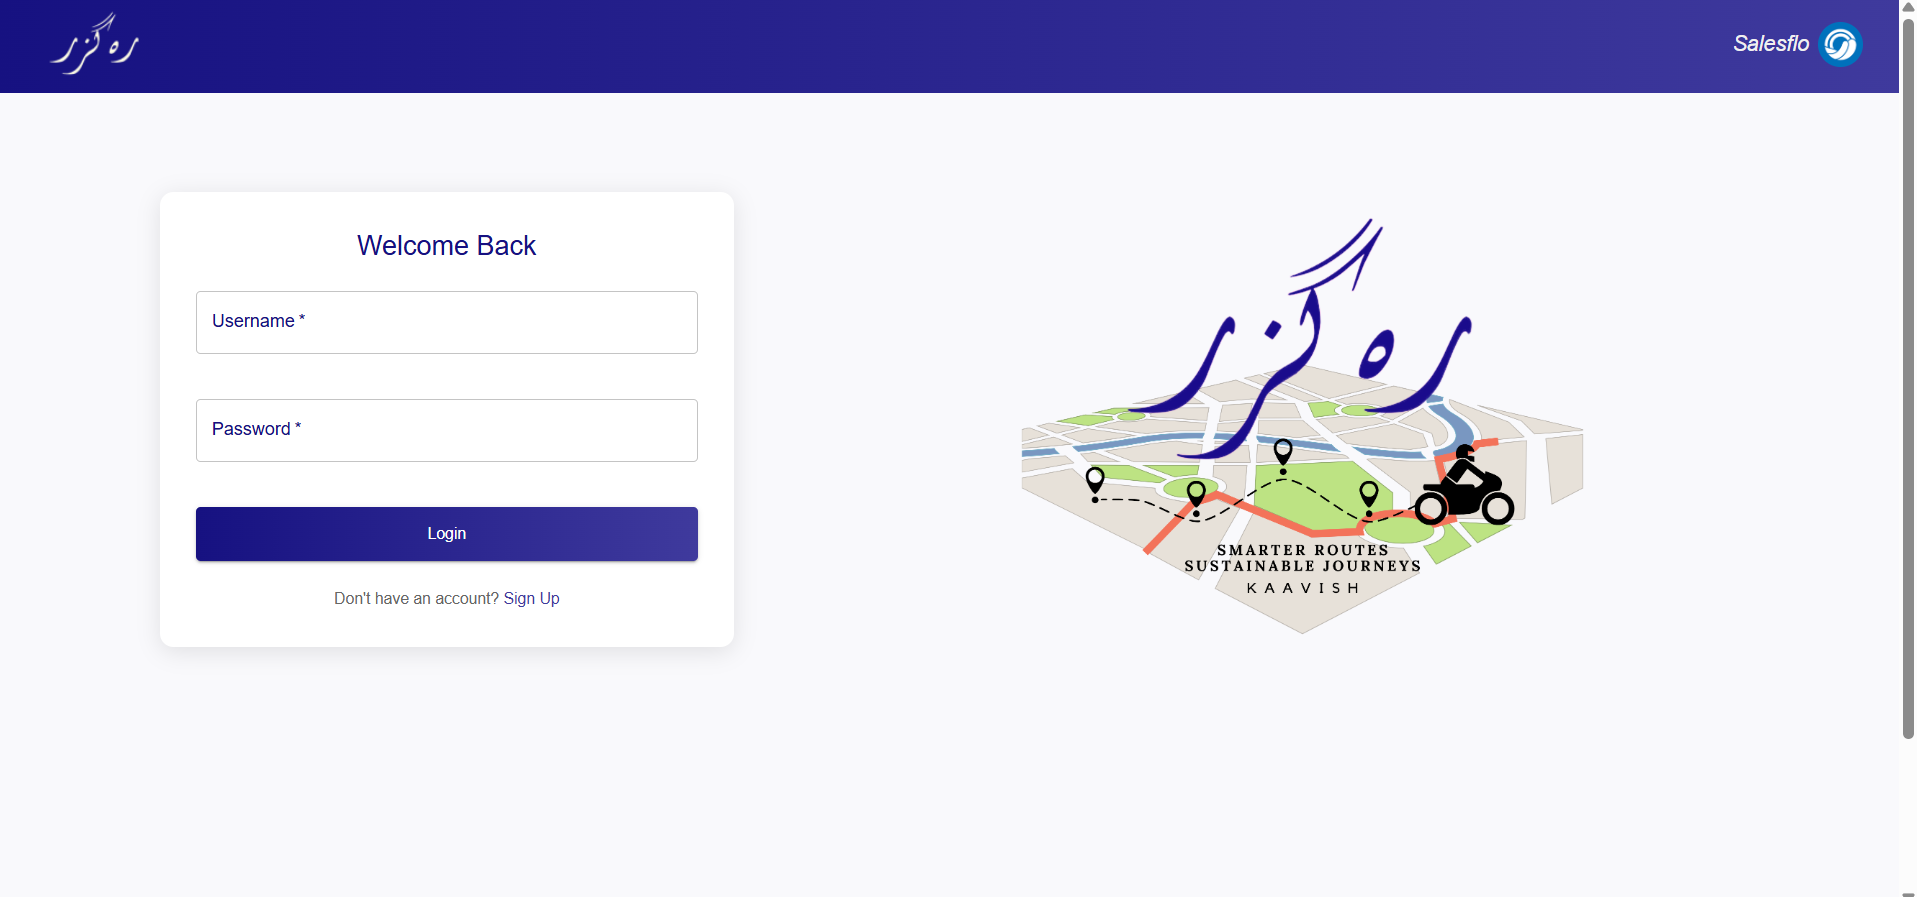
\includegraphics[width=1\textwidth]{images/Login.png} % Adjust width as needed
    \caption{Login Screen}
    \label{fig:image1}
\end{figure}
The login screen is shown in Figure~\ref{fig:image1}, letting the user enter their username and password to login.


\begin{figure}[H]
    \centering
    \includegraphics[width=1\textwidth]{images/StartScreen.png} % Adjust width as needed
    \caption{Home Page}
    \label{fig:image3}
\end{figure}
The ``Home Page" screen is shown in Figure~\ref{fig:image3}. The Route plan generator is the main screen where the instructions to start are provided.


\begin{figure}[H]
    \centering
    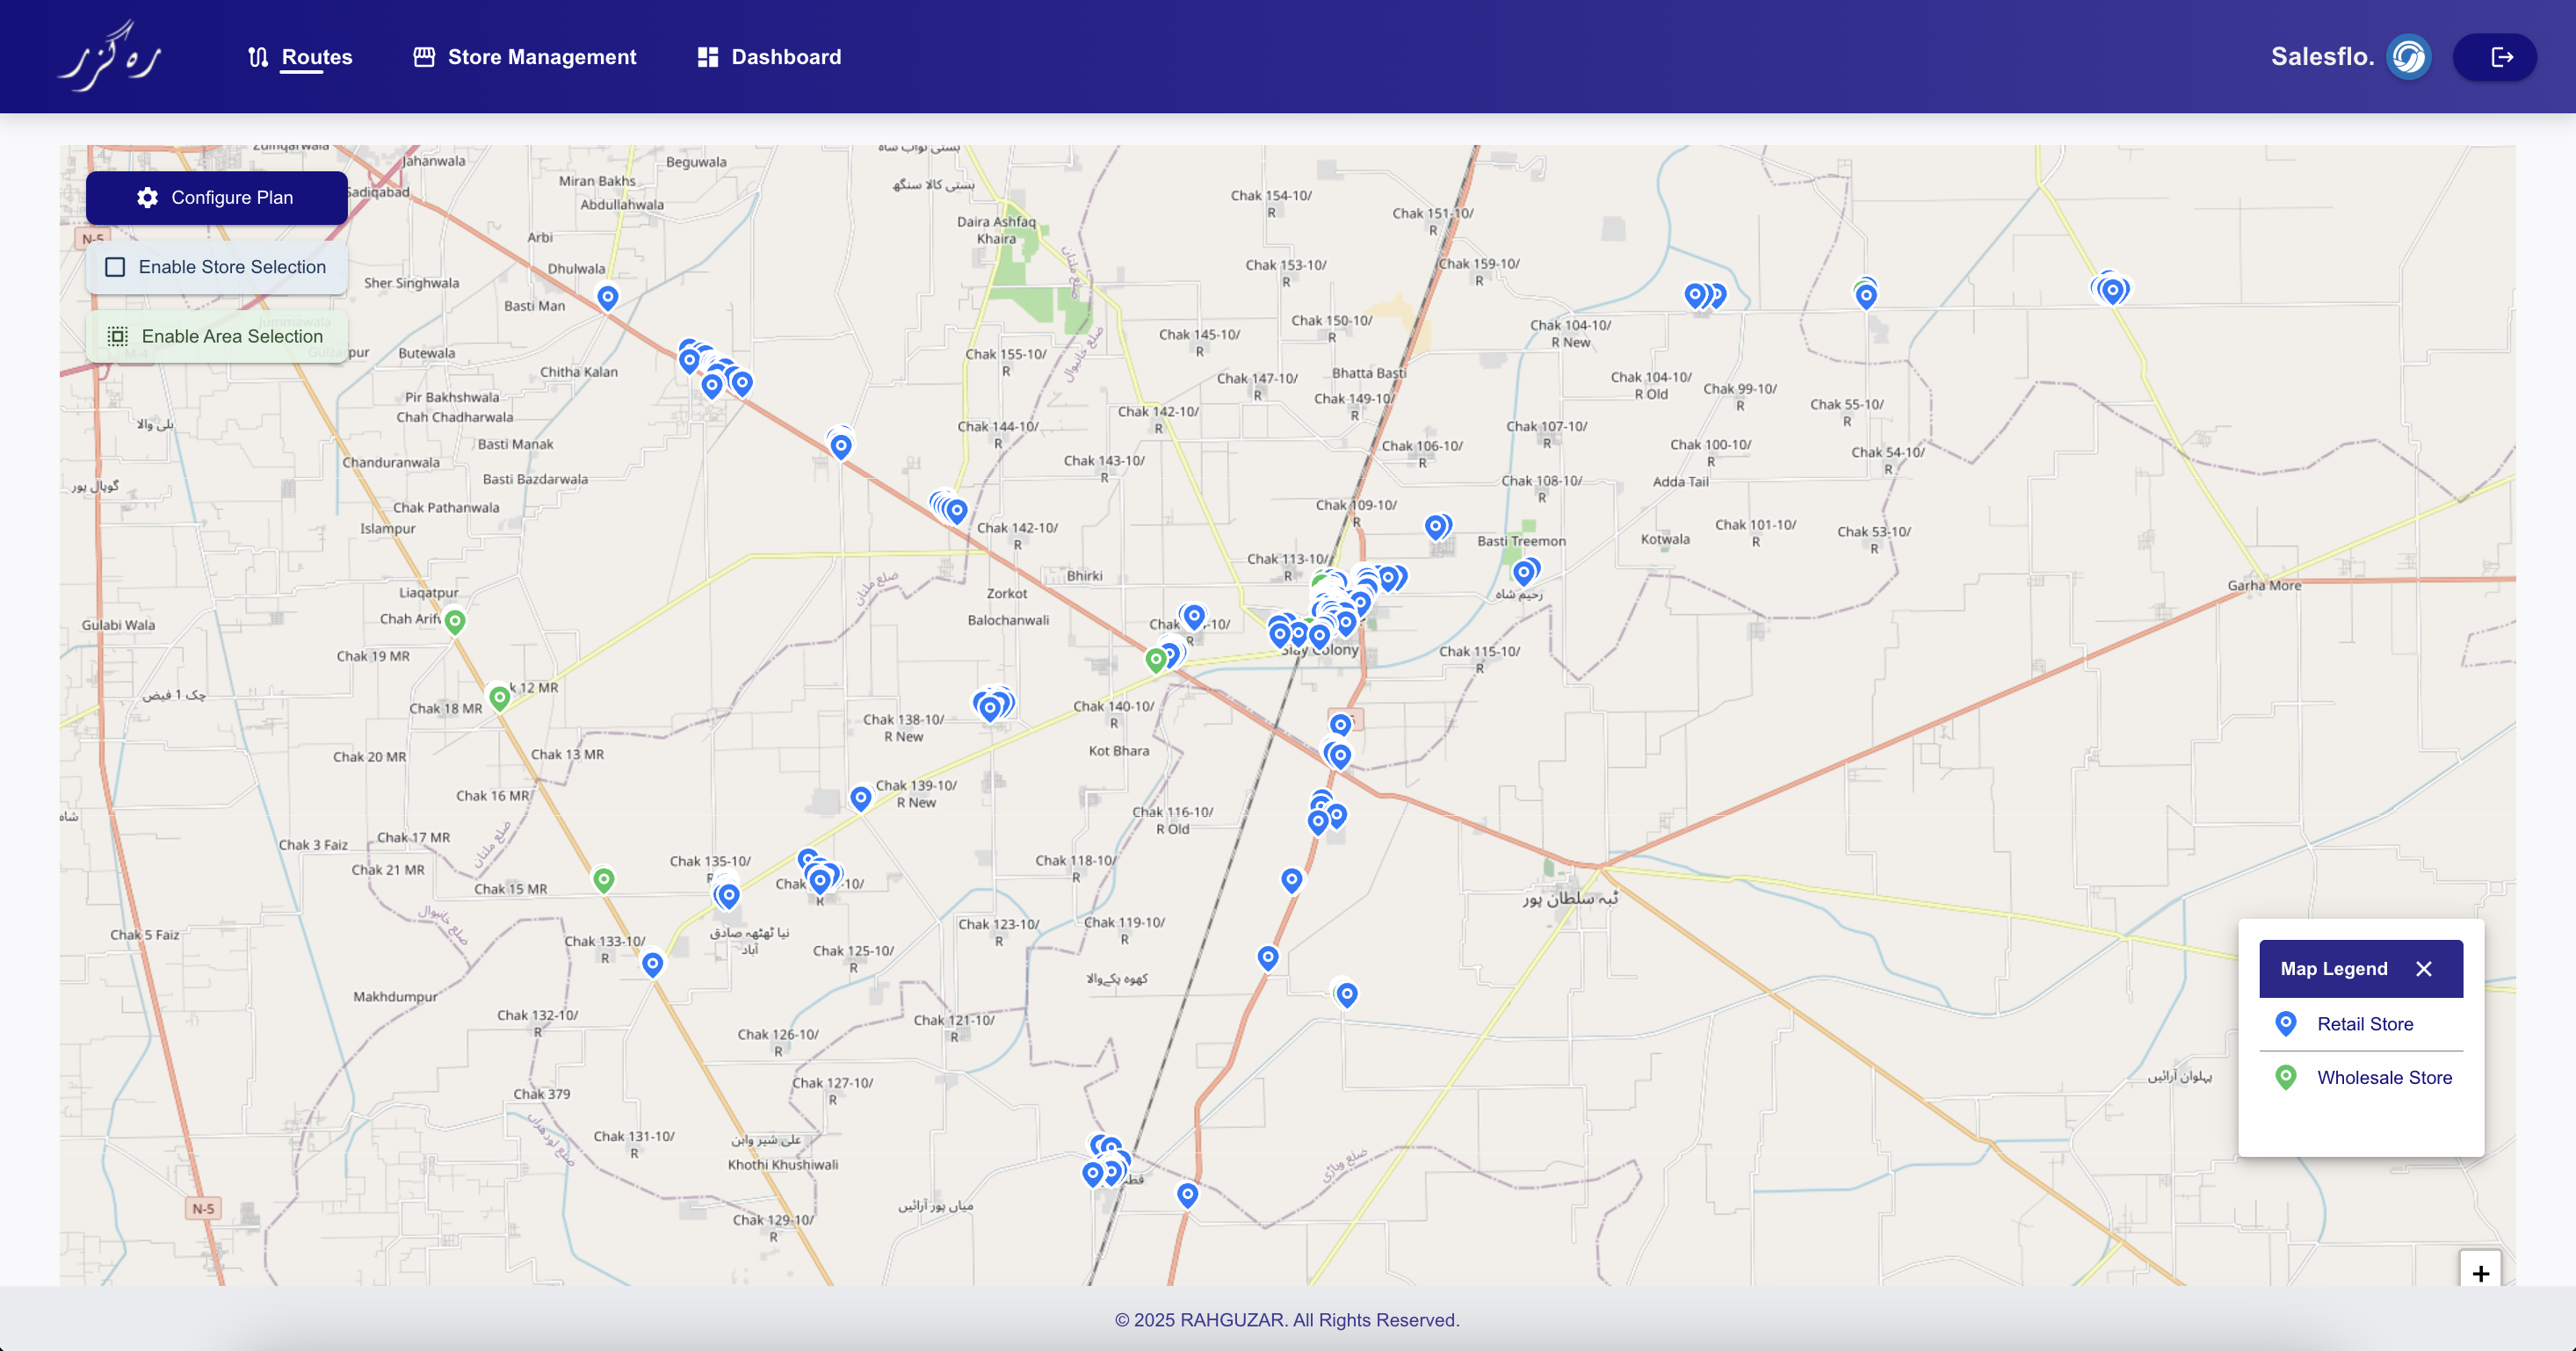
\includegraphics[width=1\textwidth]{images/Map.png} % Adjust width as needed
    \caption{Plan Route Page}
    \label{fig:image4}
\end{figure}
The ``Map" screen is shown in Figure~\ref{fig:image4}. In this screen, the manager will be able to view the map and the stores on it. The manager can select stores using area selection or point selection which will be used in the plan.


\begin{figure}[H]
    \centering
    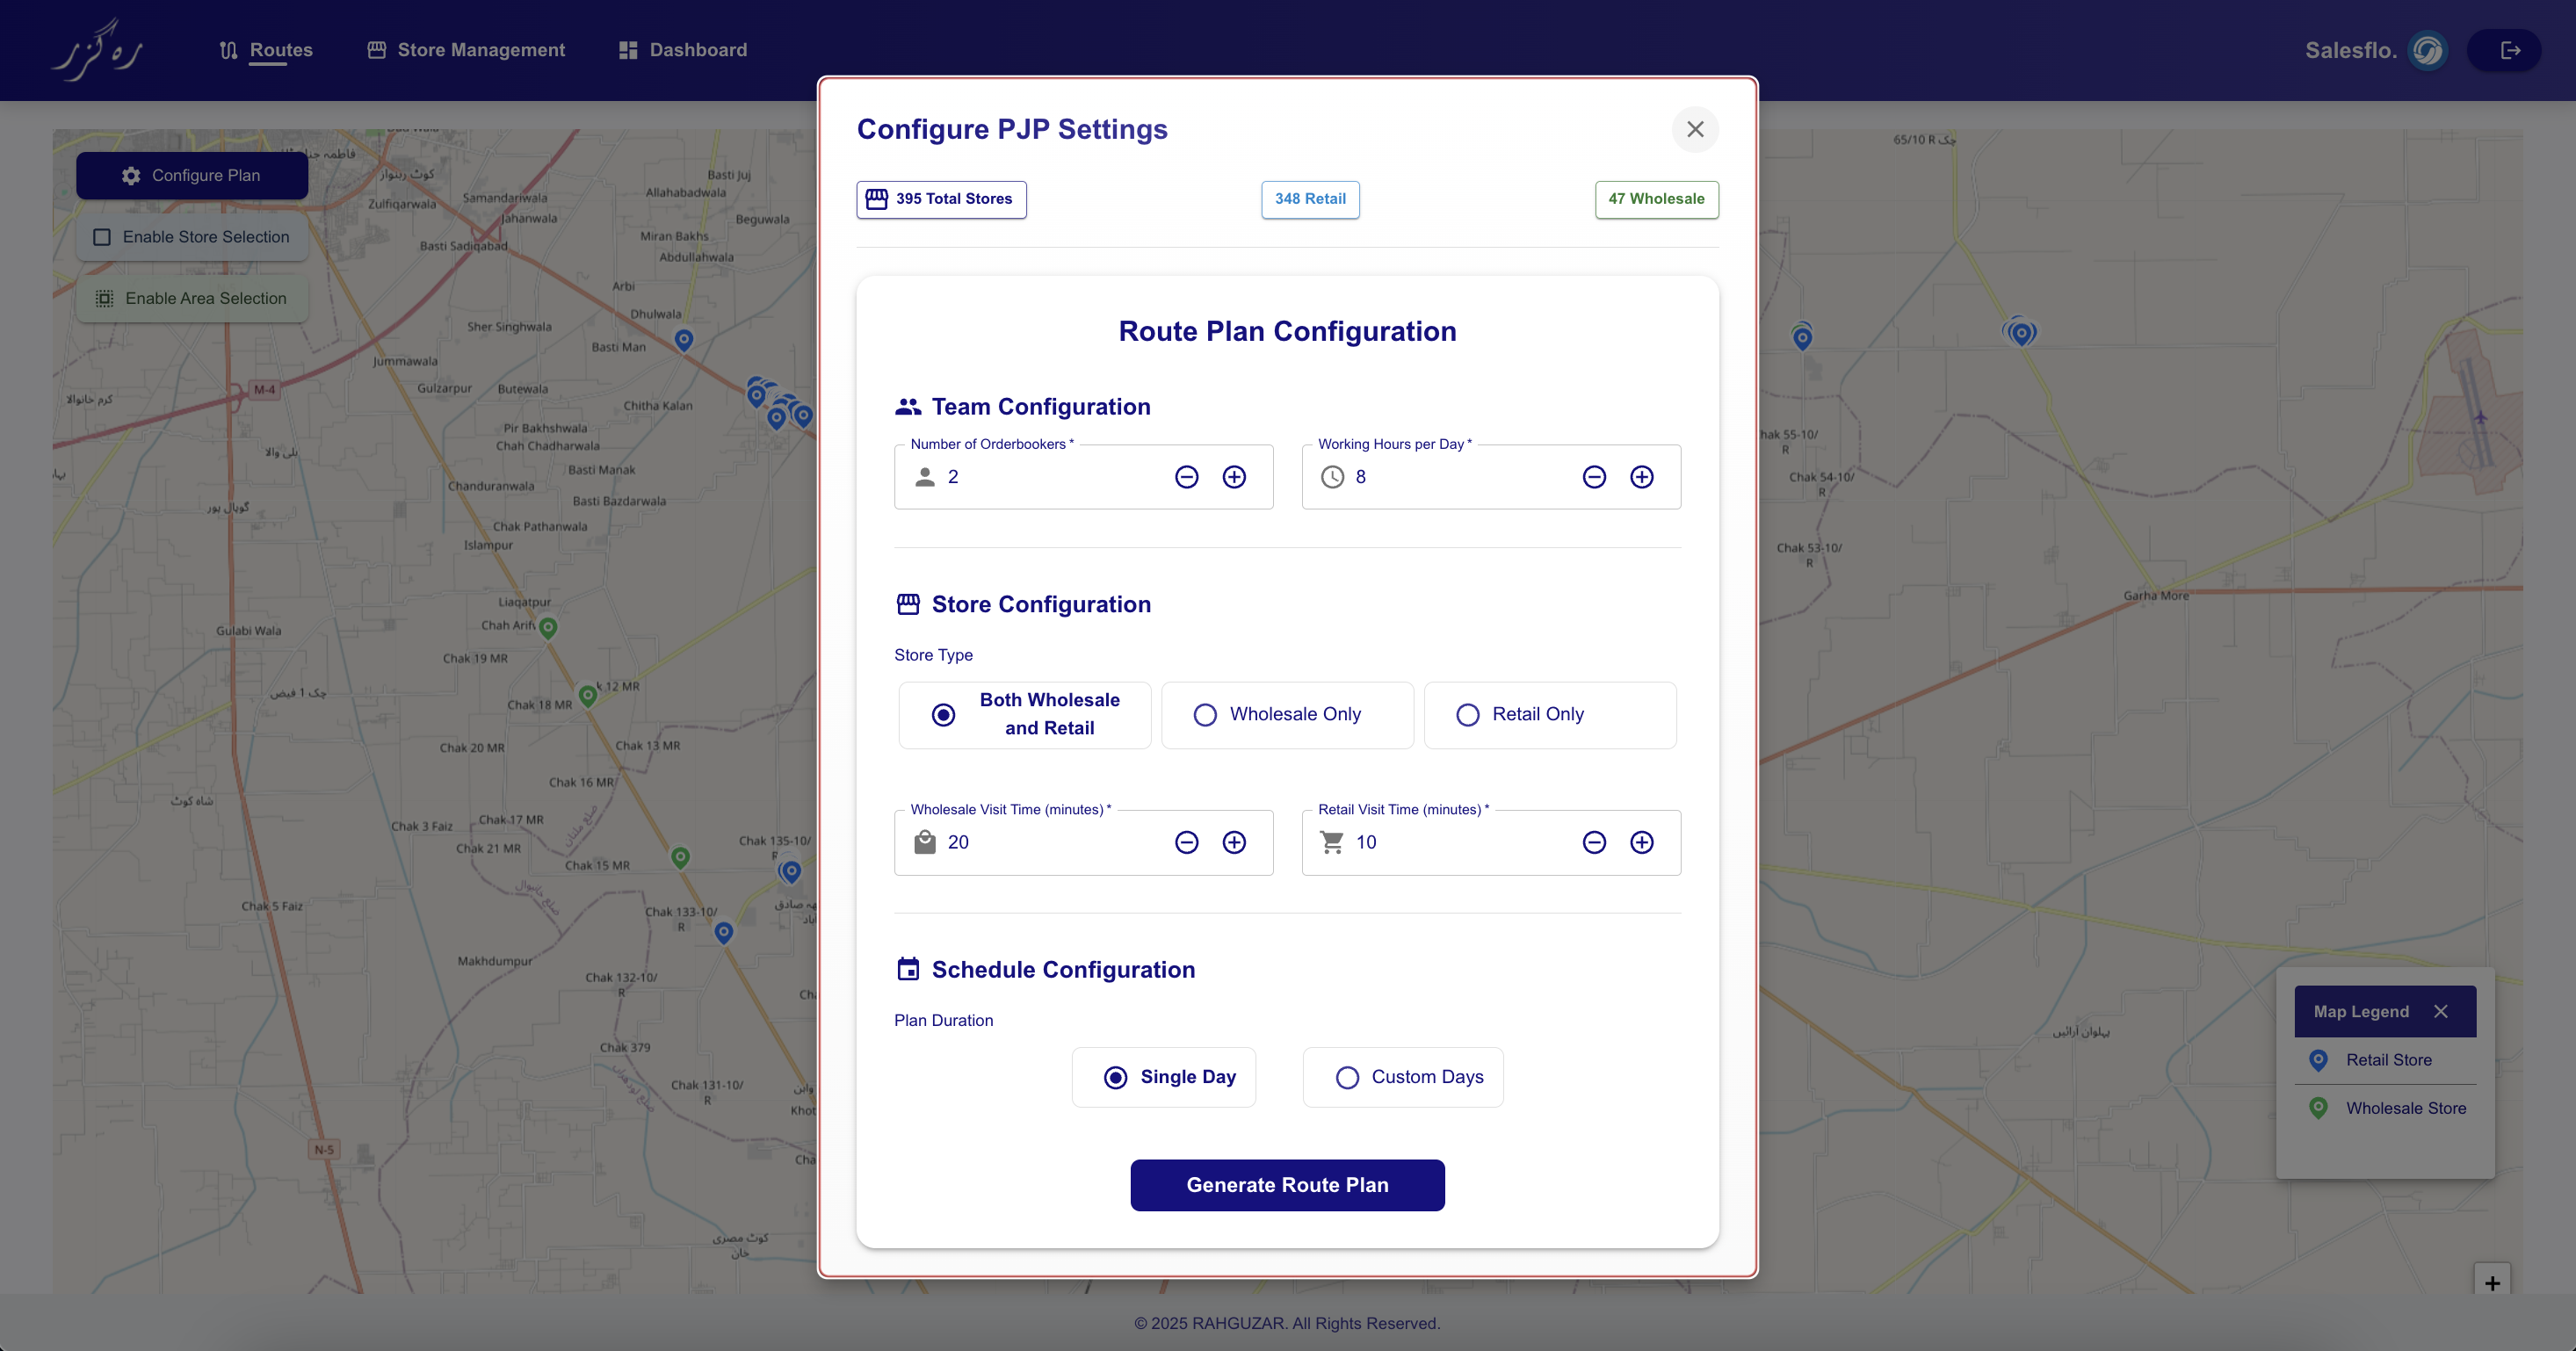
\includegraphics[width=1\textwidth]{images/Configure.png} % Adjust width as needed
    \caption{Configure Route Parameters}
    \label{fig:image4}
\end{figure}
The manager can configure the route parameters in the ``Configure Route" screen shown in Figure~\ref{fig:image4}. In this screen, the manager will be able to set the shift timings, number of order bookers, and the number of stores to visit. The manager can also set the travel time and service time for each store.

\begin{figure}[H]
    \centering
    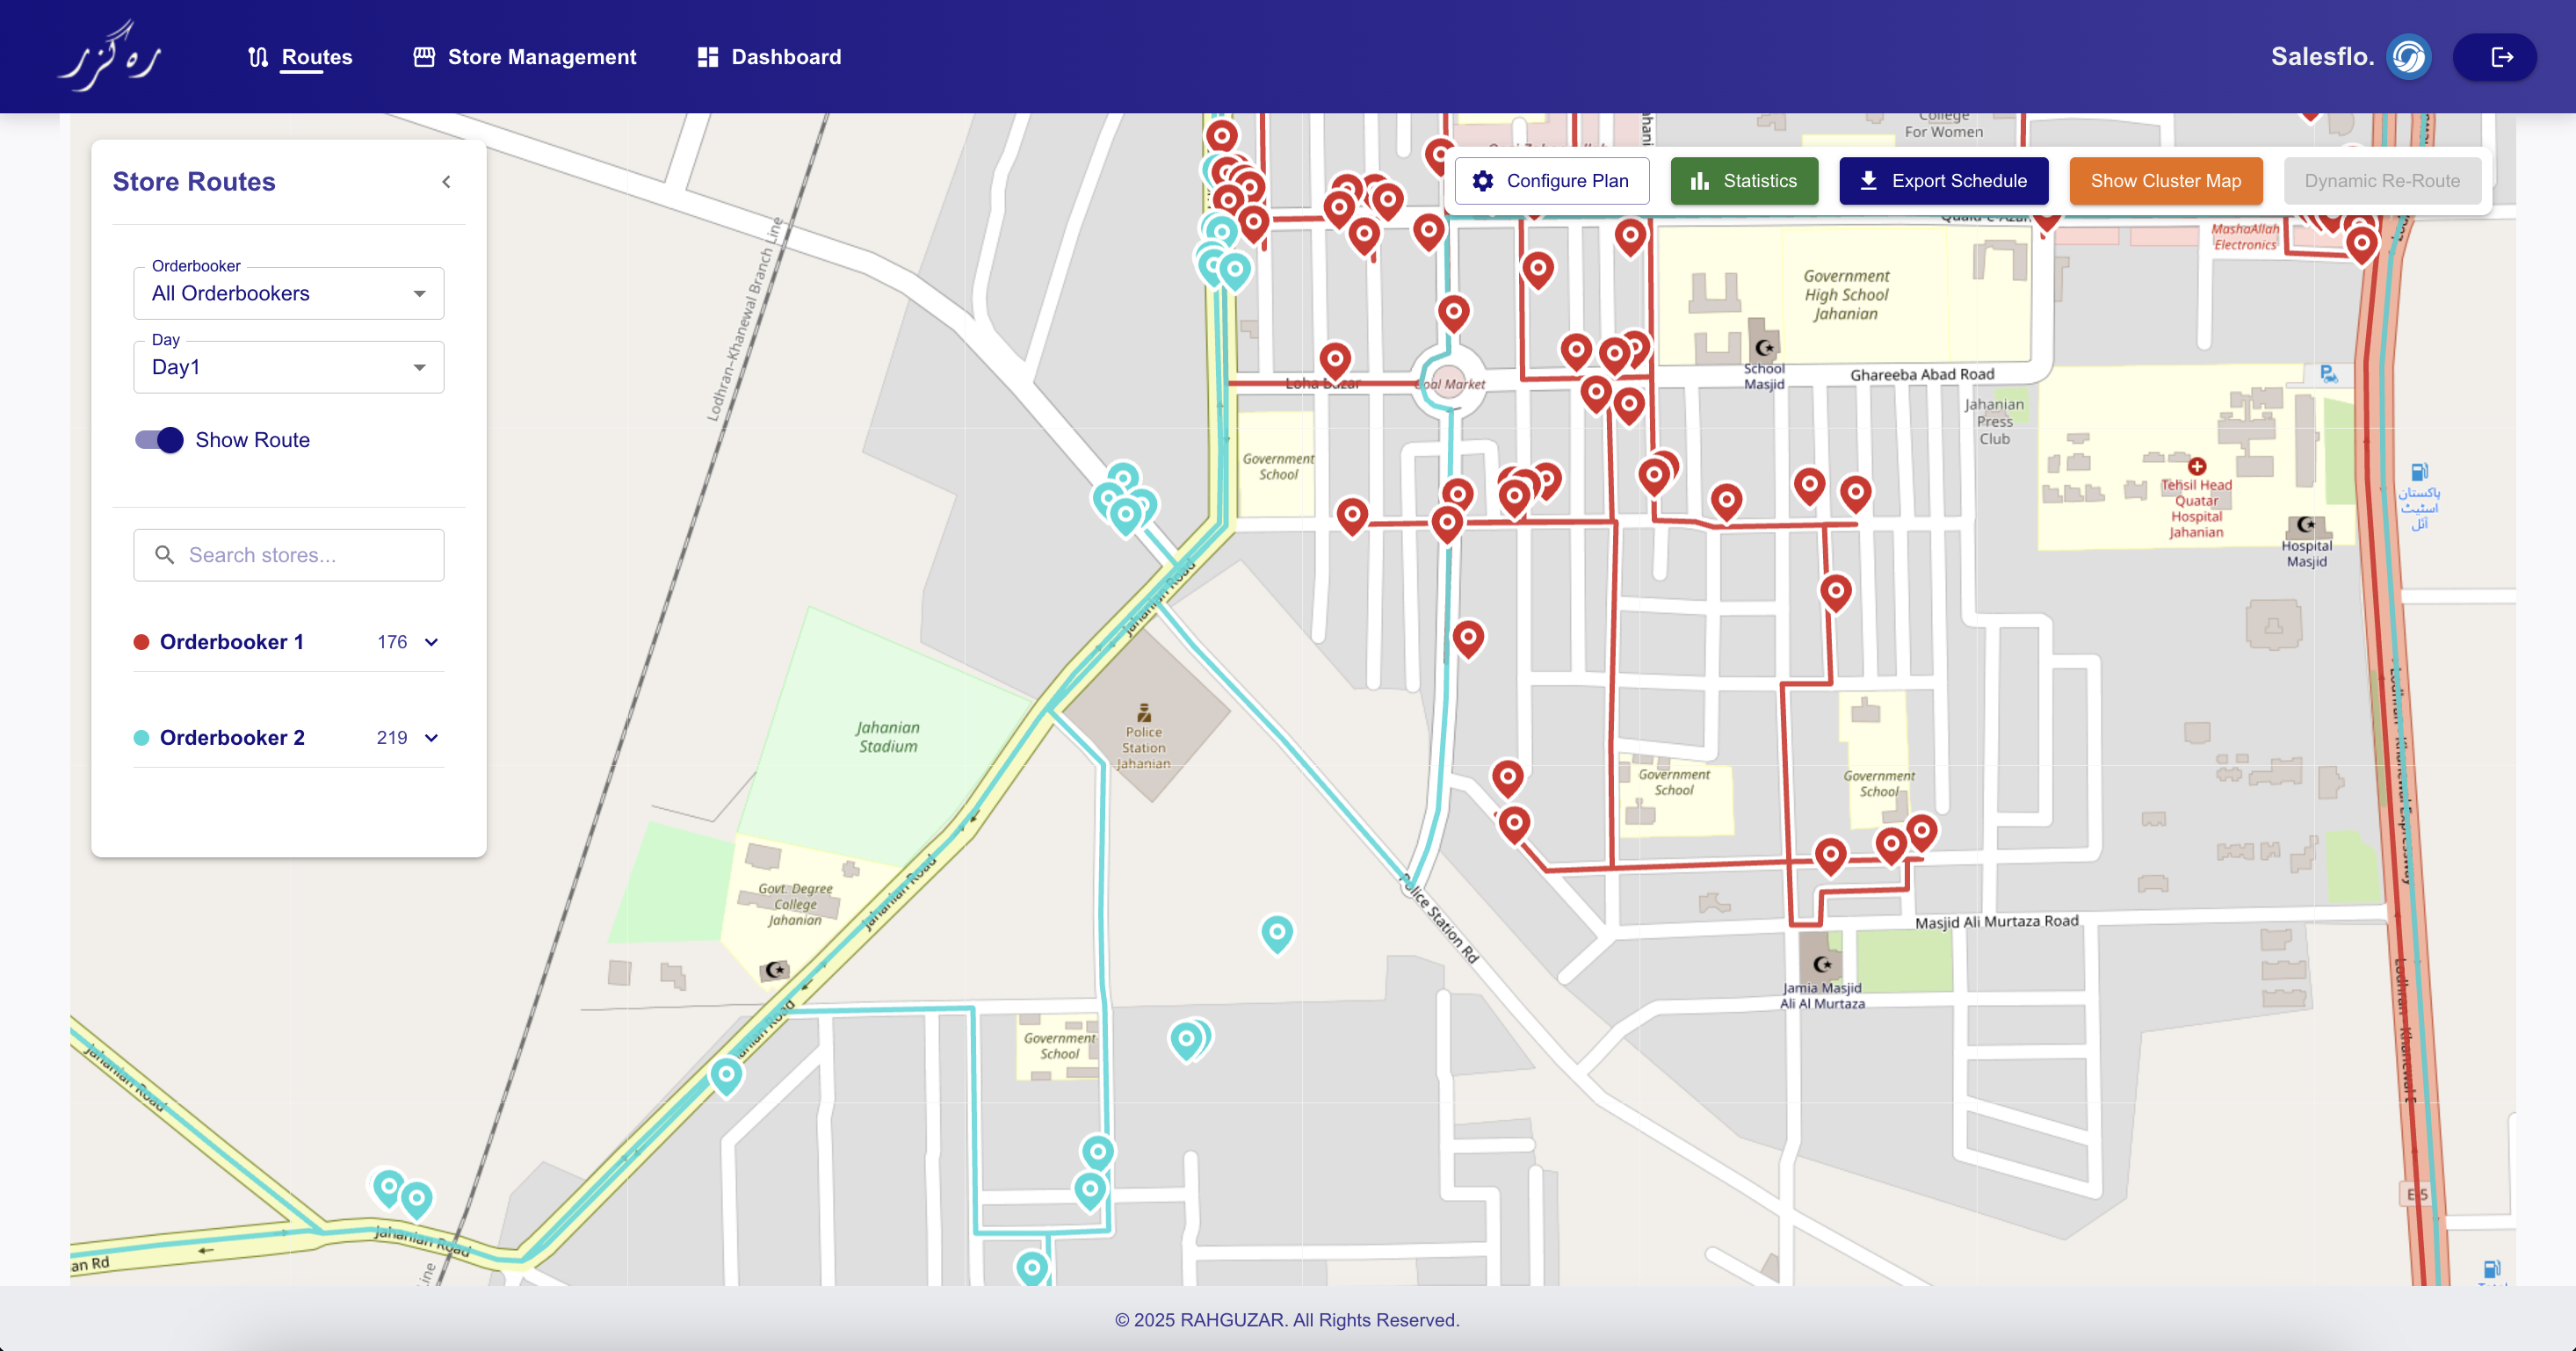
\includegraphics[width=1\textwidth]{images/plan.png} % Adjust width as needed
    \caption{View Routes Page}
    \label{fig:image6}
\end{figure}
The ``Plan Route" screen is shown in Figure~\ref{fig:image6}. In this screen, the manager will be able to view the routes generated by the system. The manager can also view the route details such as the distance, travel time, and service time for each store. The manager can also view the route on the map and download it in a CSV format.

\begin{figure}[H]
    \centering
    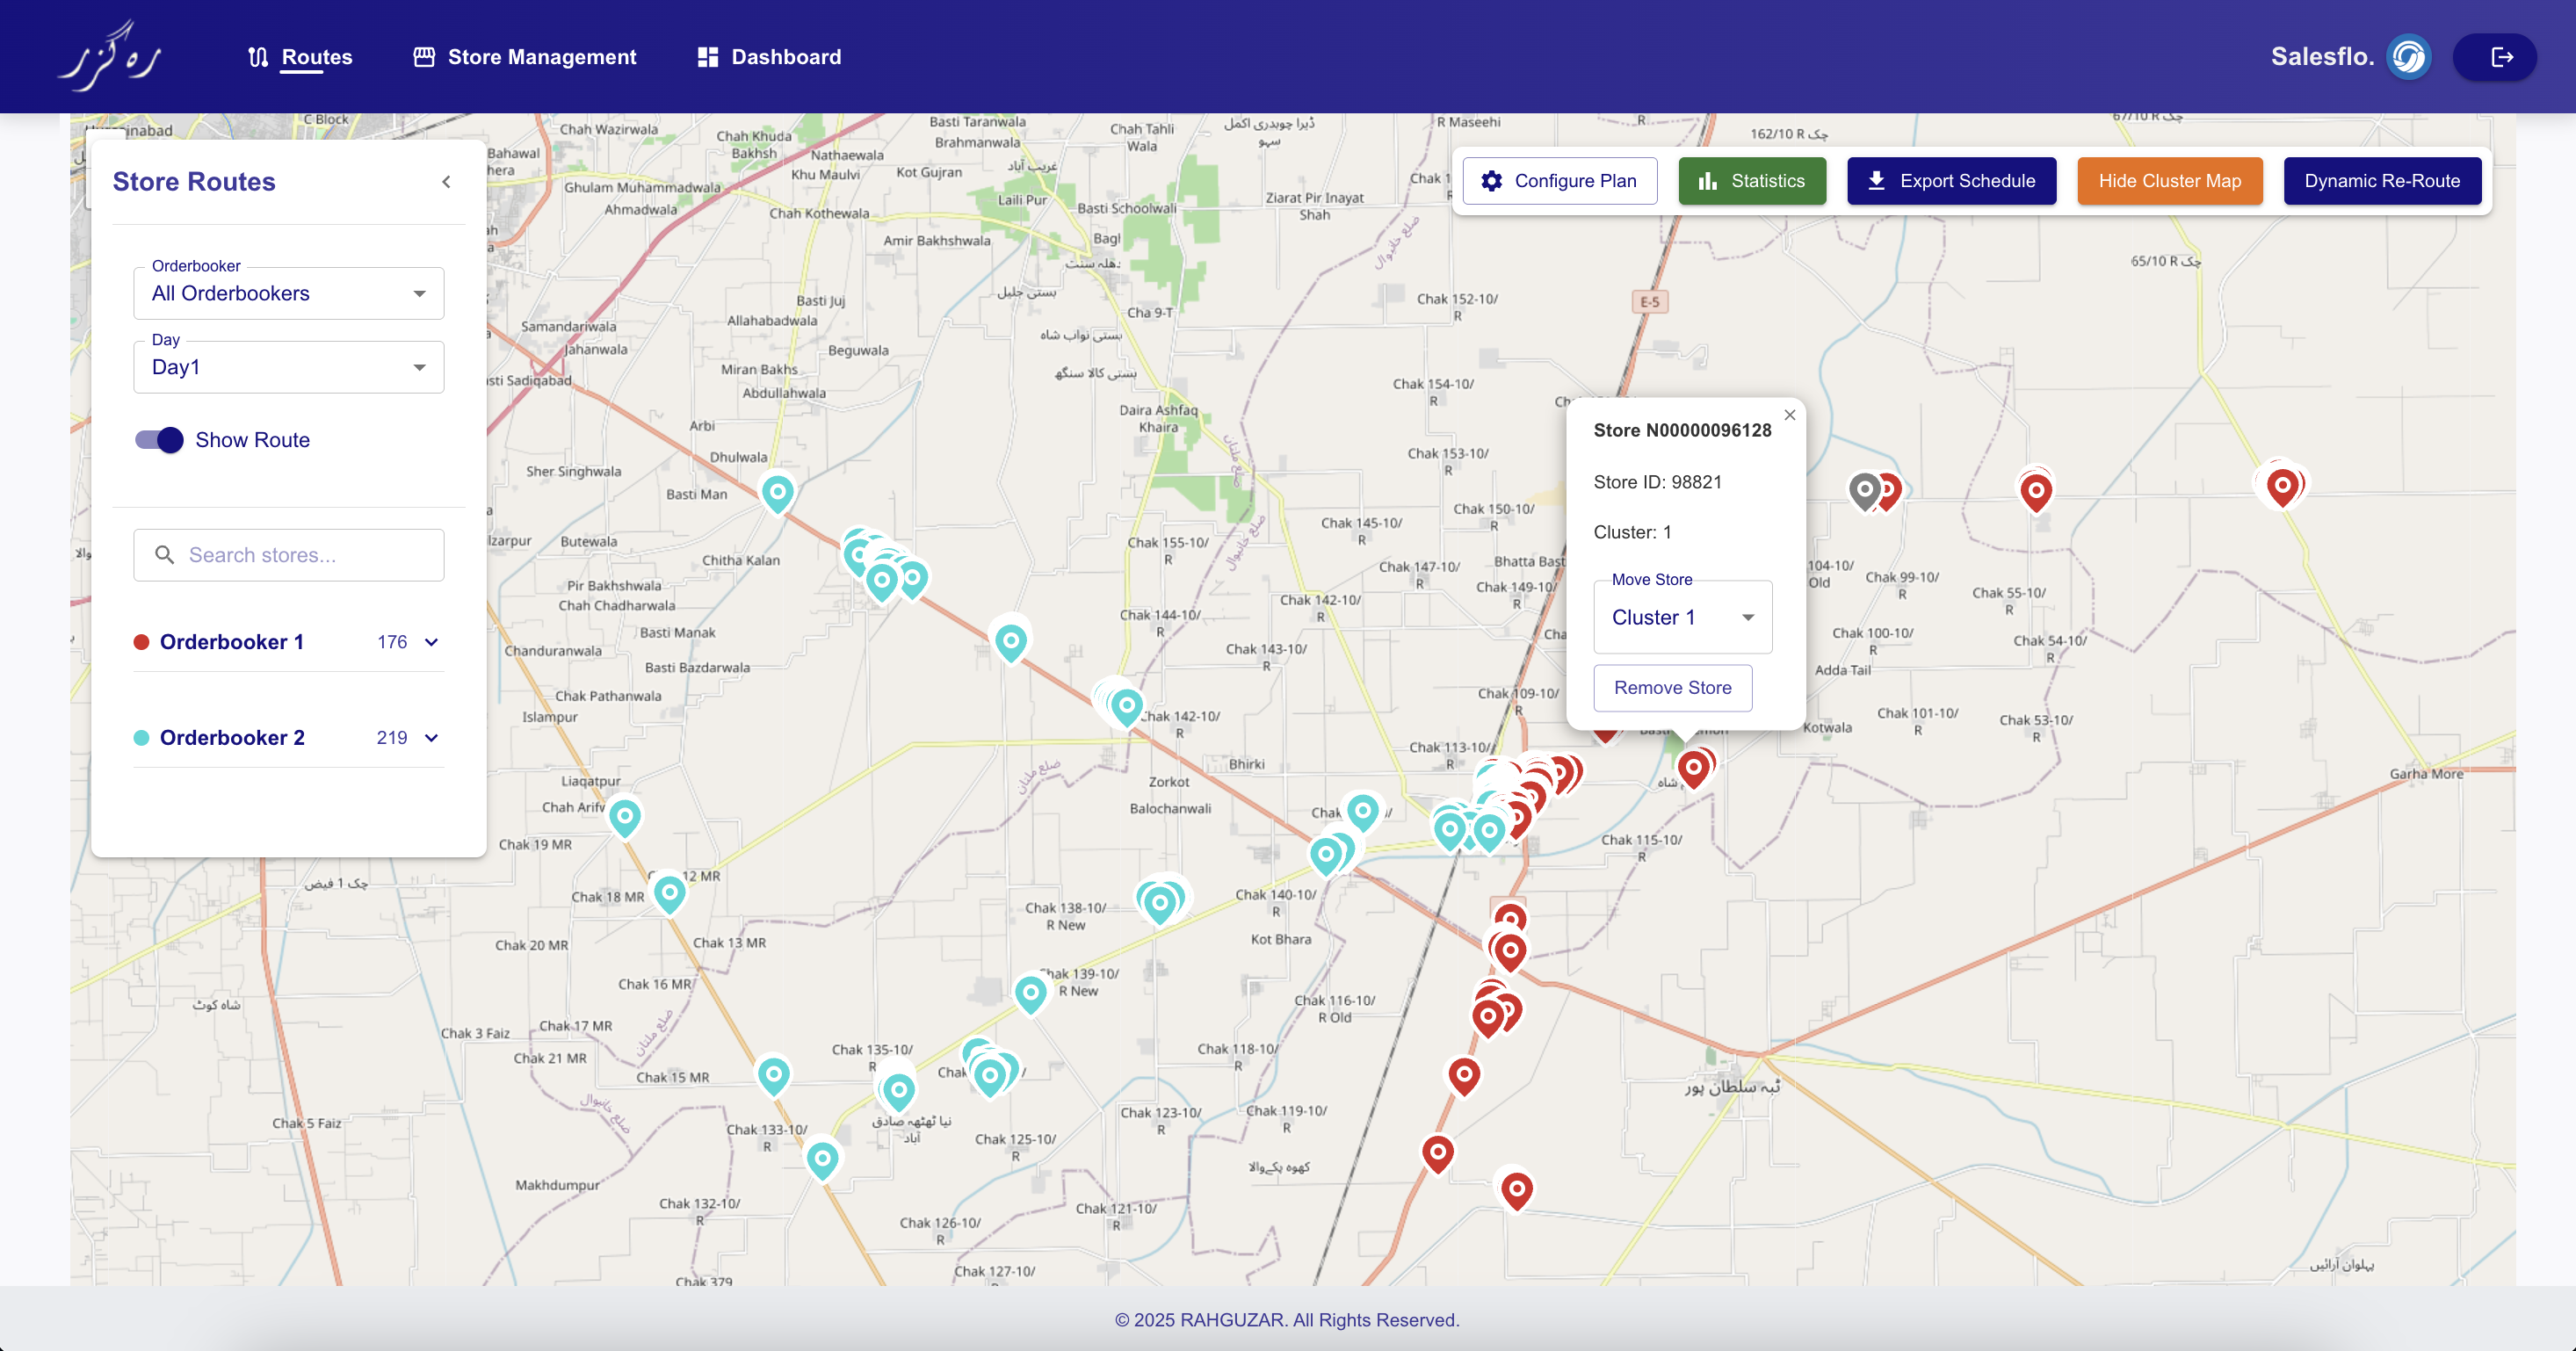
\includegraphics[width=1\textwidth]{images/Cluster map.png} % Adjust width as needed
    \caption{Cluster Map Page}
    \label{fig:image6}
\end{figure}
The ``Cluster Map" screen is shown in Figure~\ref{fig:image6}. In this screen, the manager will be able to view the clusters generated by the system. The manager can modify the stores in clusters by removing them or moving them to another cluster, after which they can dynamically reroute the plan.

\begin{figure}[H]
    \centering
    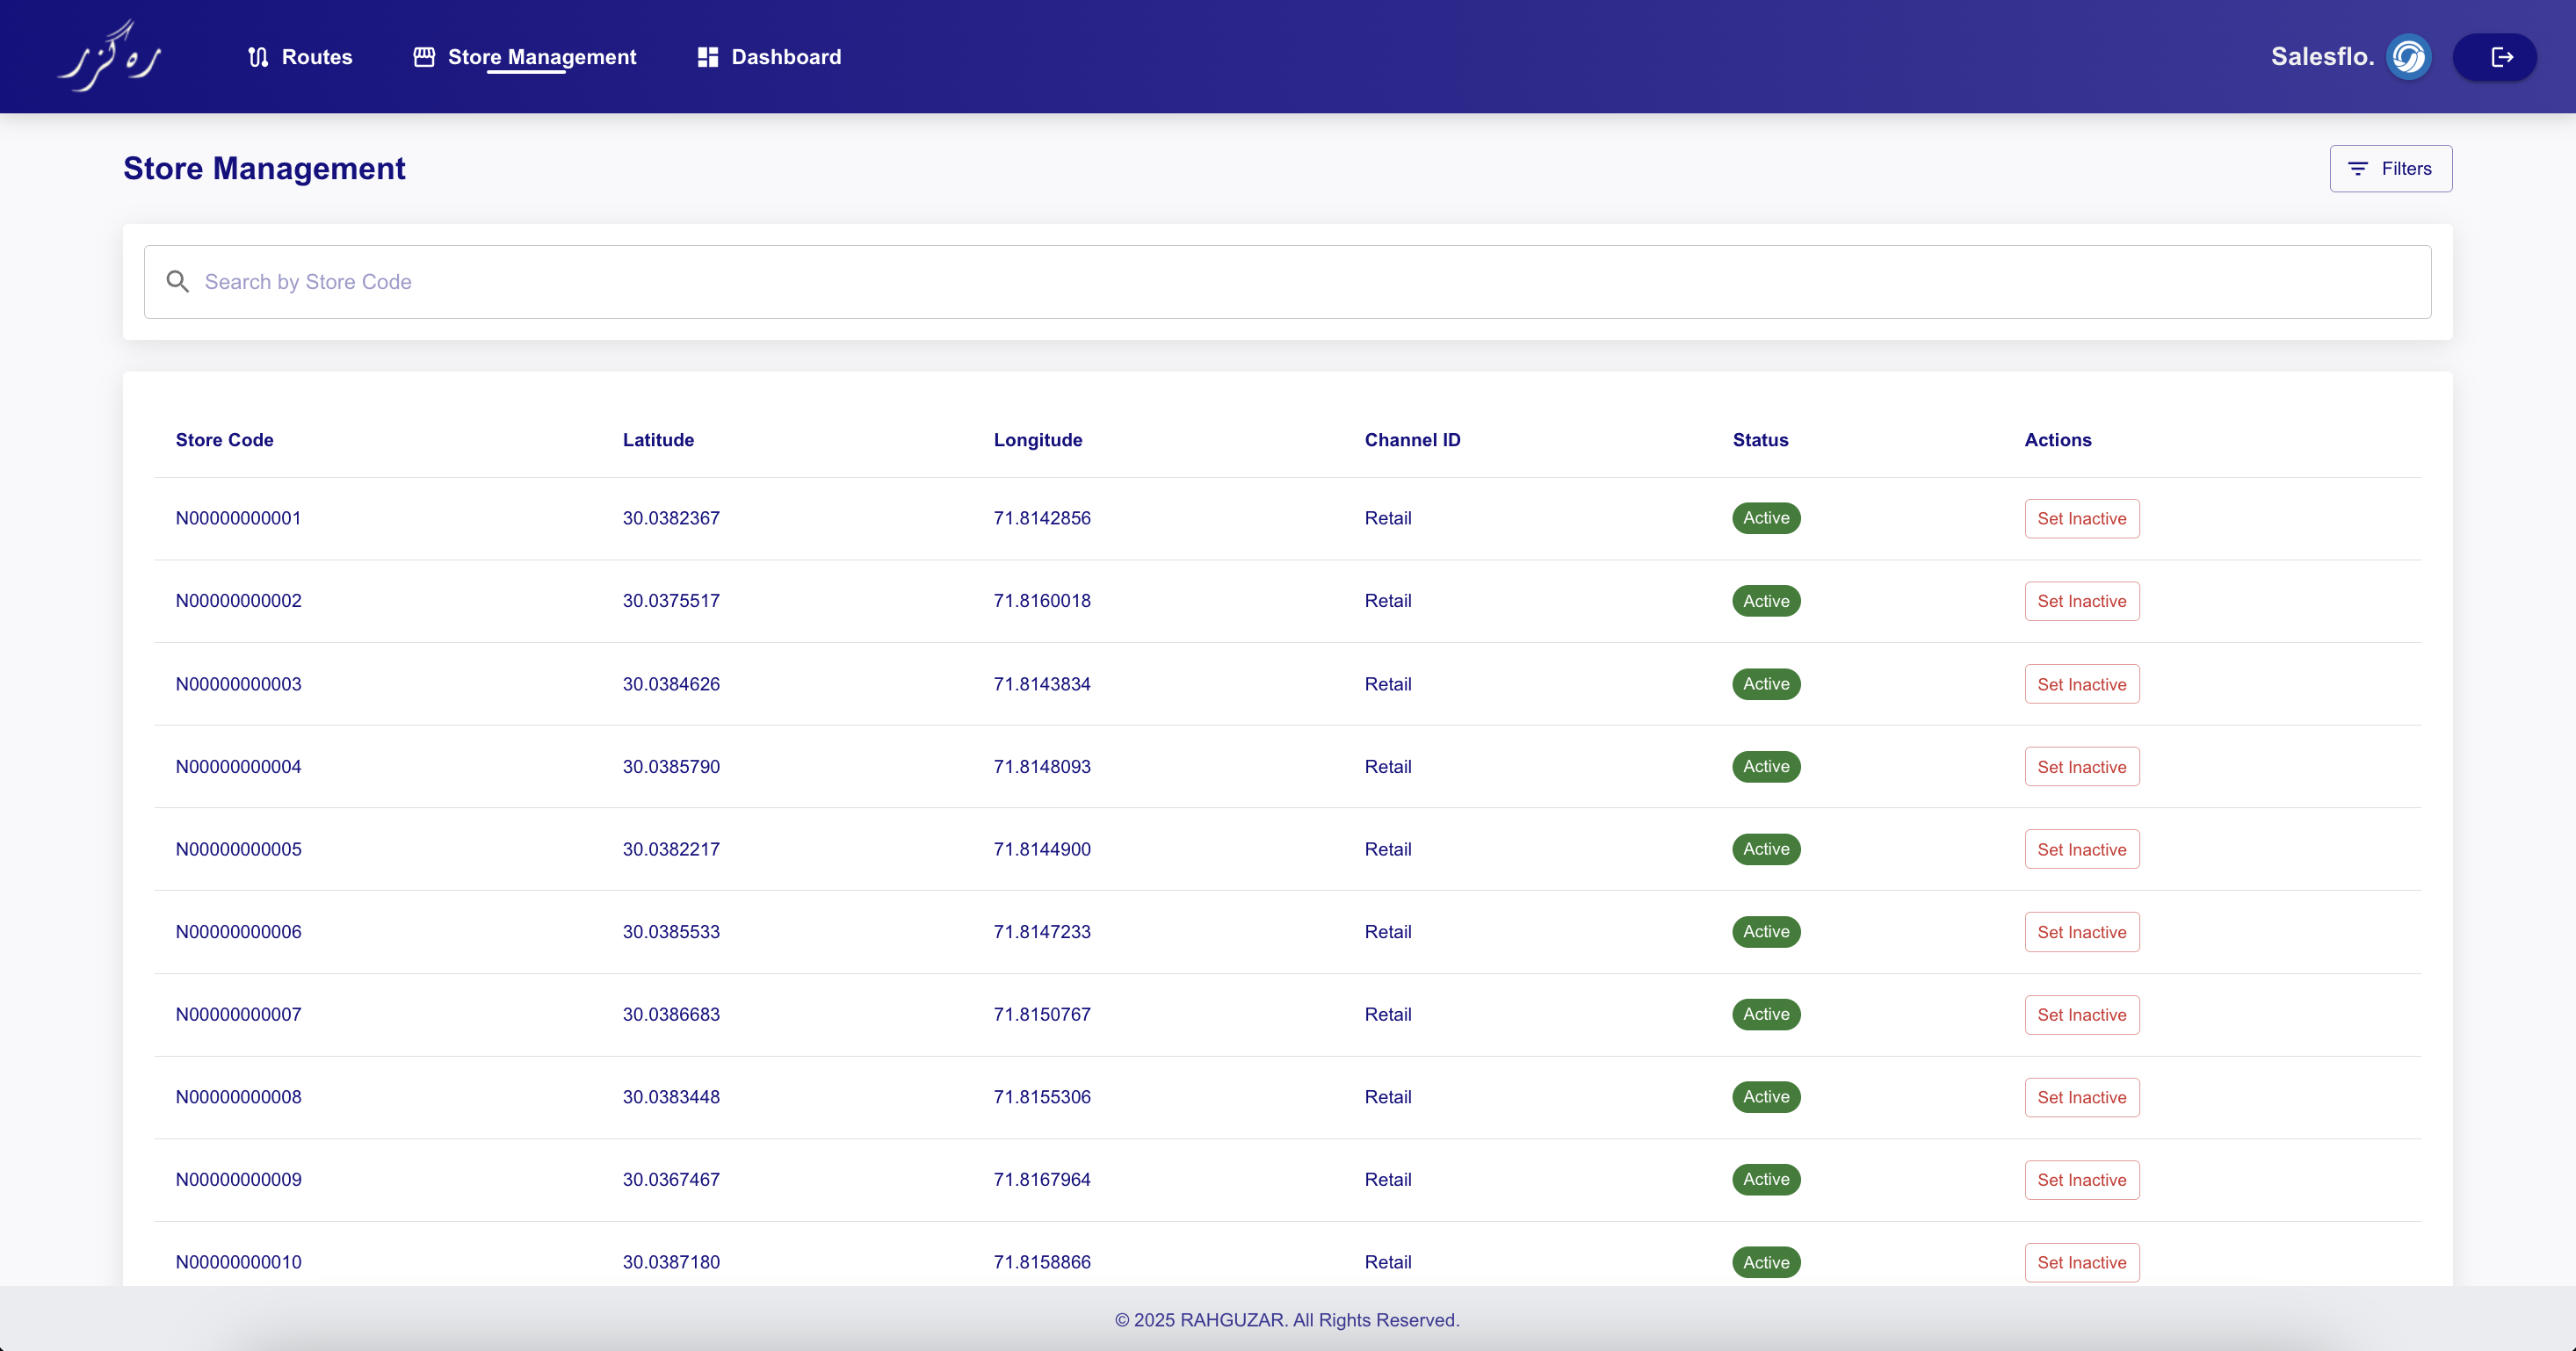
\includegraphics[width=1\textwidth]{images/stores.png} % Adjust width as needed
    \caption{Stores Management Page}
    \label{fig:image5}
\end{figure}
The "Stores Management" screen is shown in Figure~\ref{fig:image5}. In this screen, the manager will be able to search a certain store, apply filters in their search, and view its information such as its coordinates. The manager has the option to view more than 1 store's information at a time, and to decide to set a store active or inactive.

\begin{figure}[H]
    \centering
    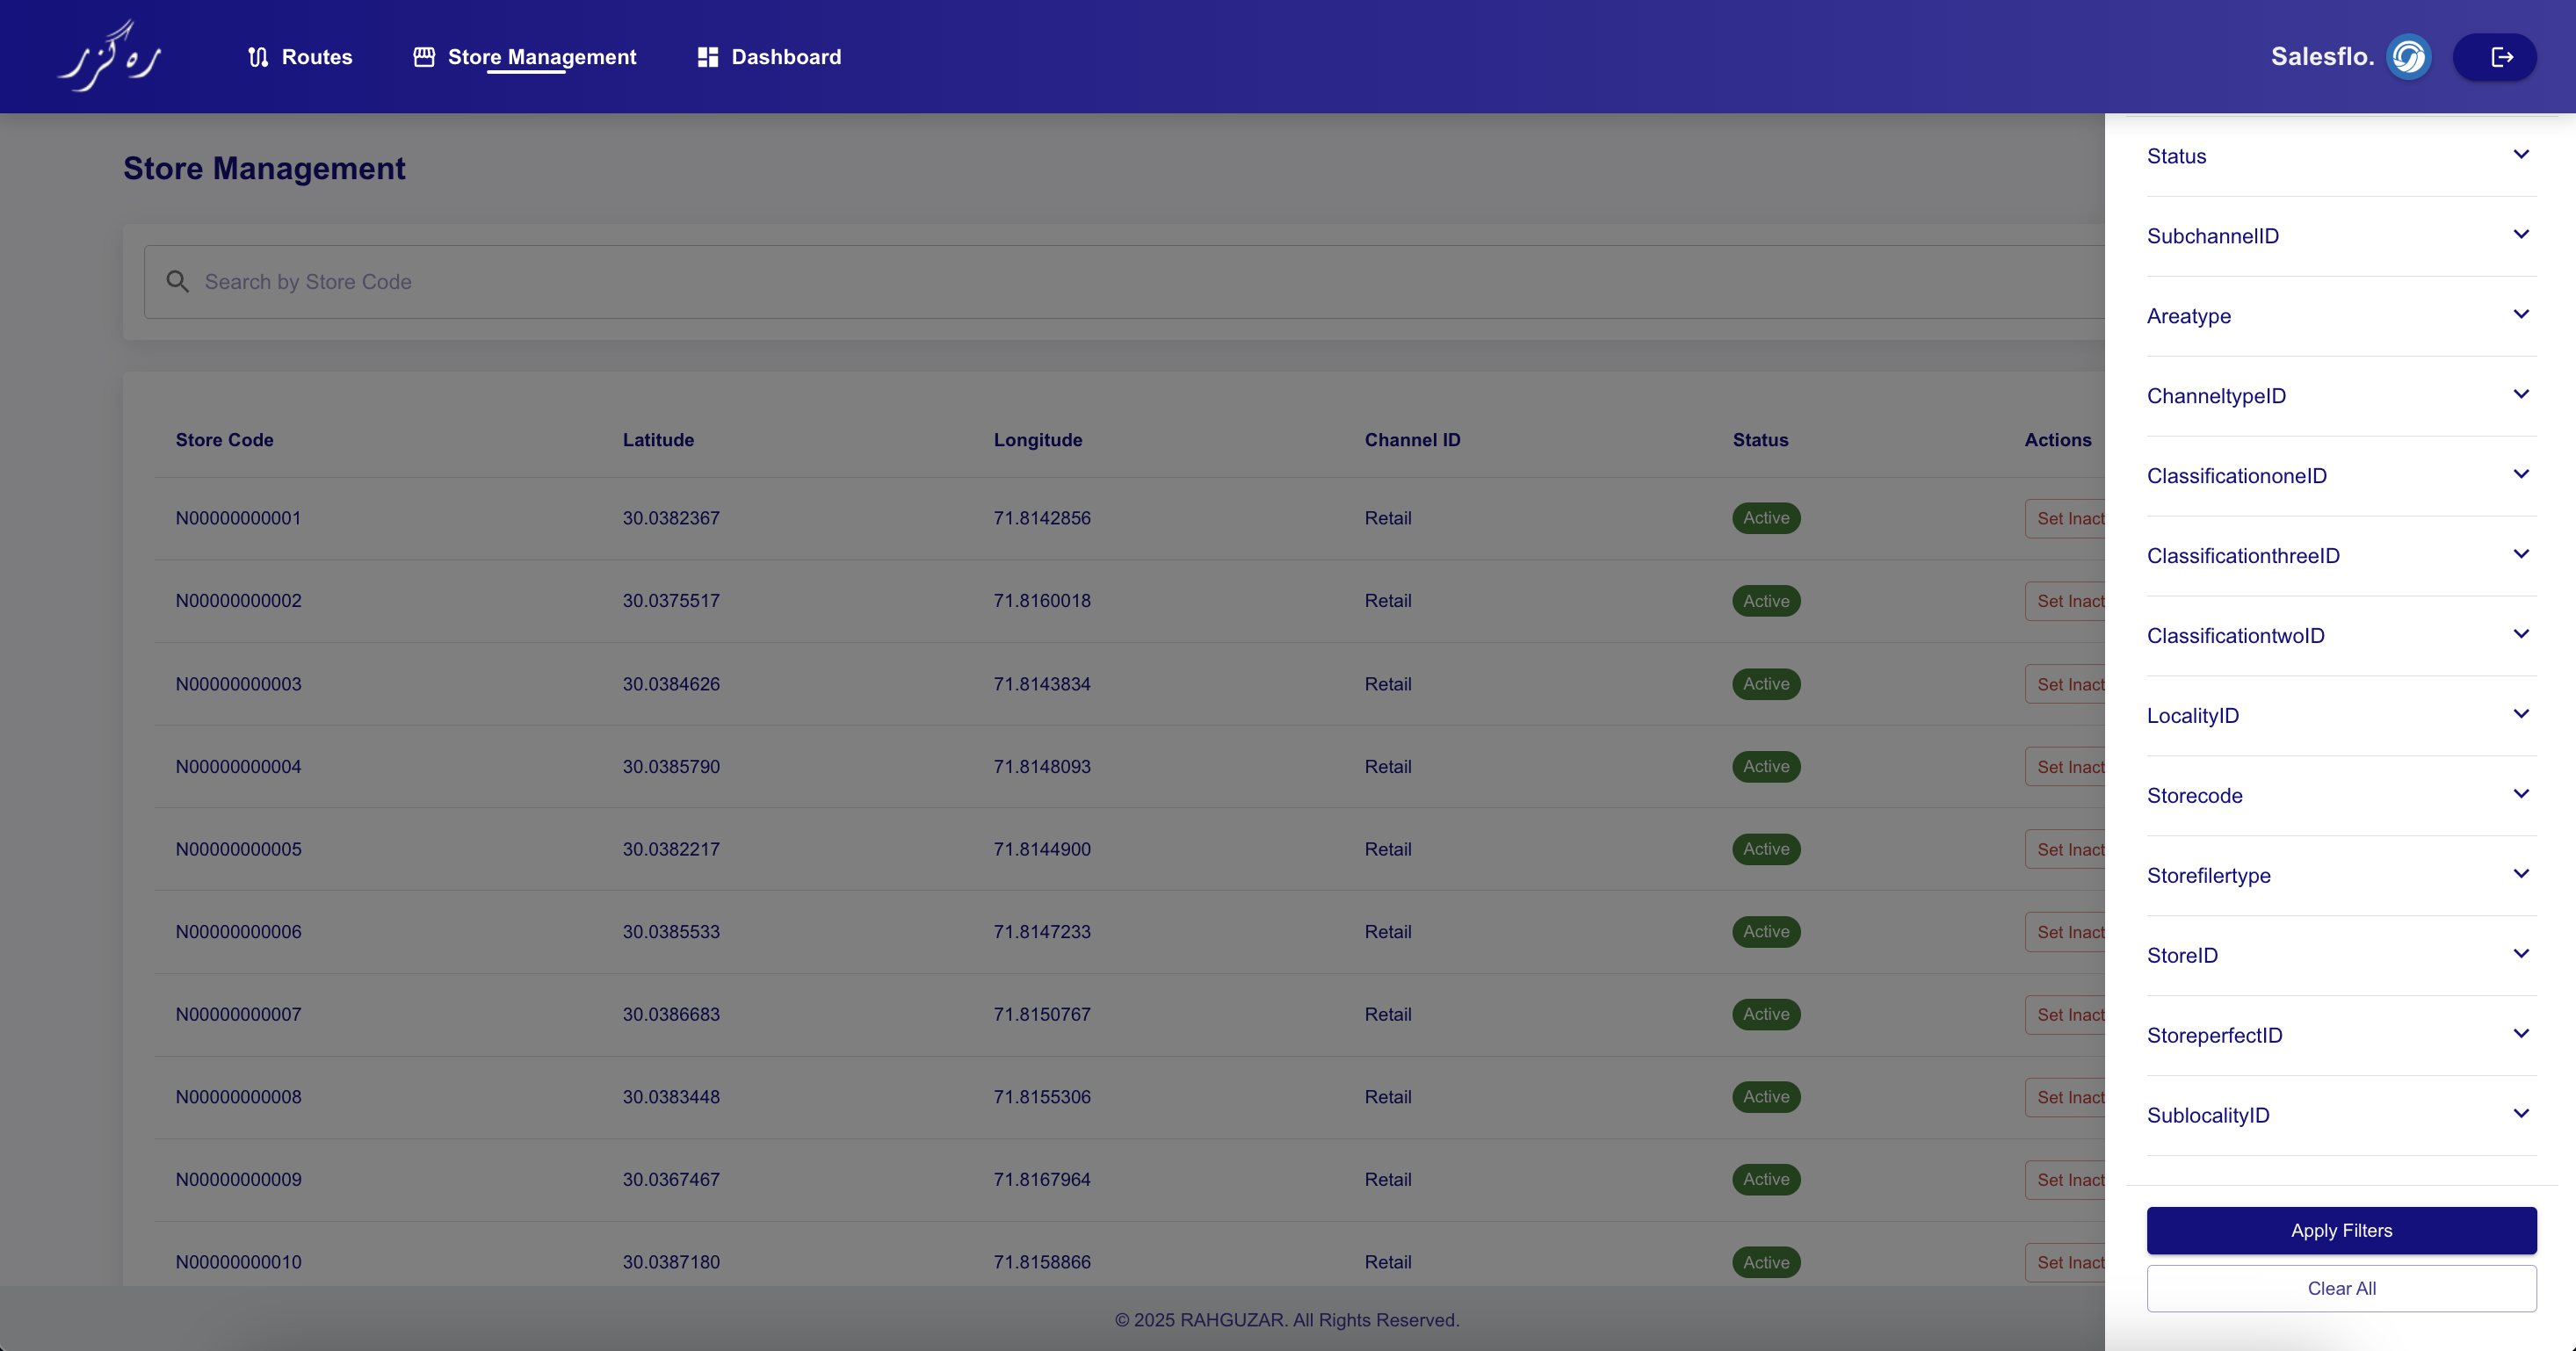
\includegraphics[width=1\textwidth]{images/store filters.png} % Adjust width as needed
    \caption{Store Filters}
    \label{fig:image6}
\end{figure}
The ``Store Filters" screen is shown in Figure~\ref{fig:image6}. In this screen, the manager will be able to view the filters applied to the stores.

\begin{figure}[H]
    \centering
    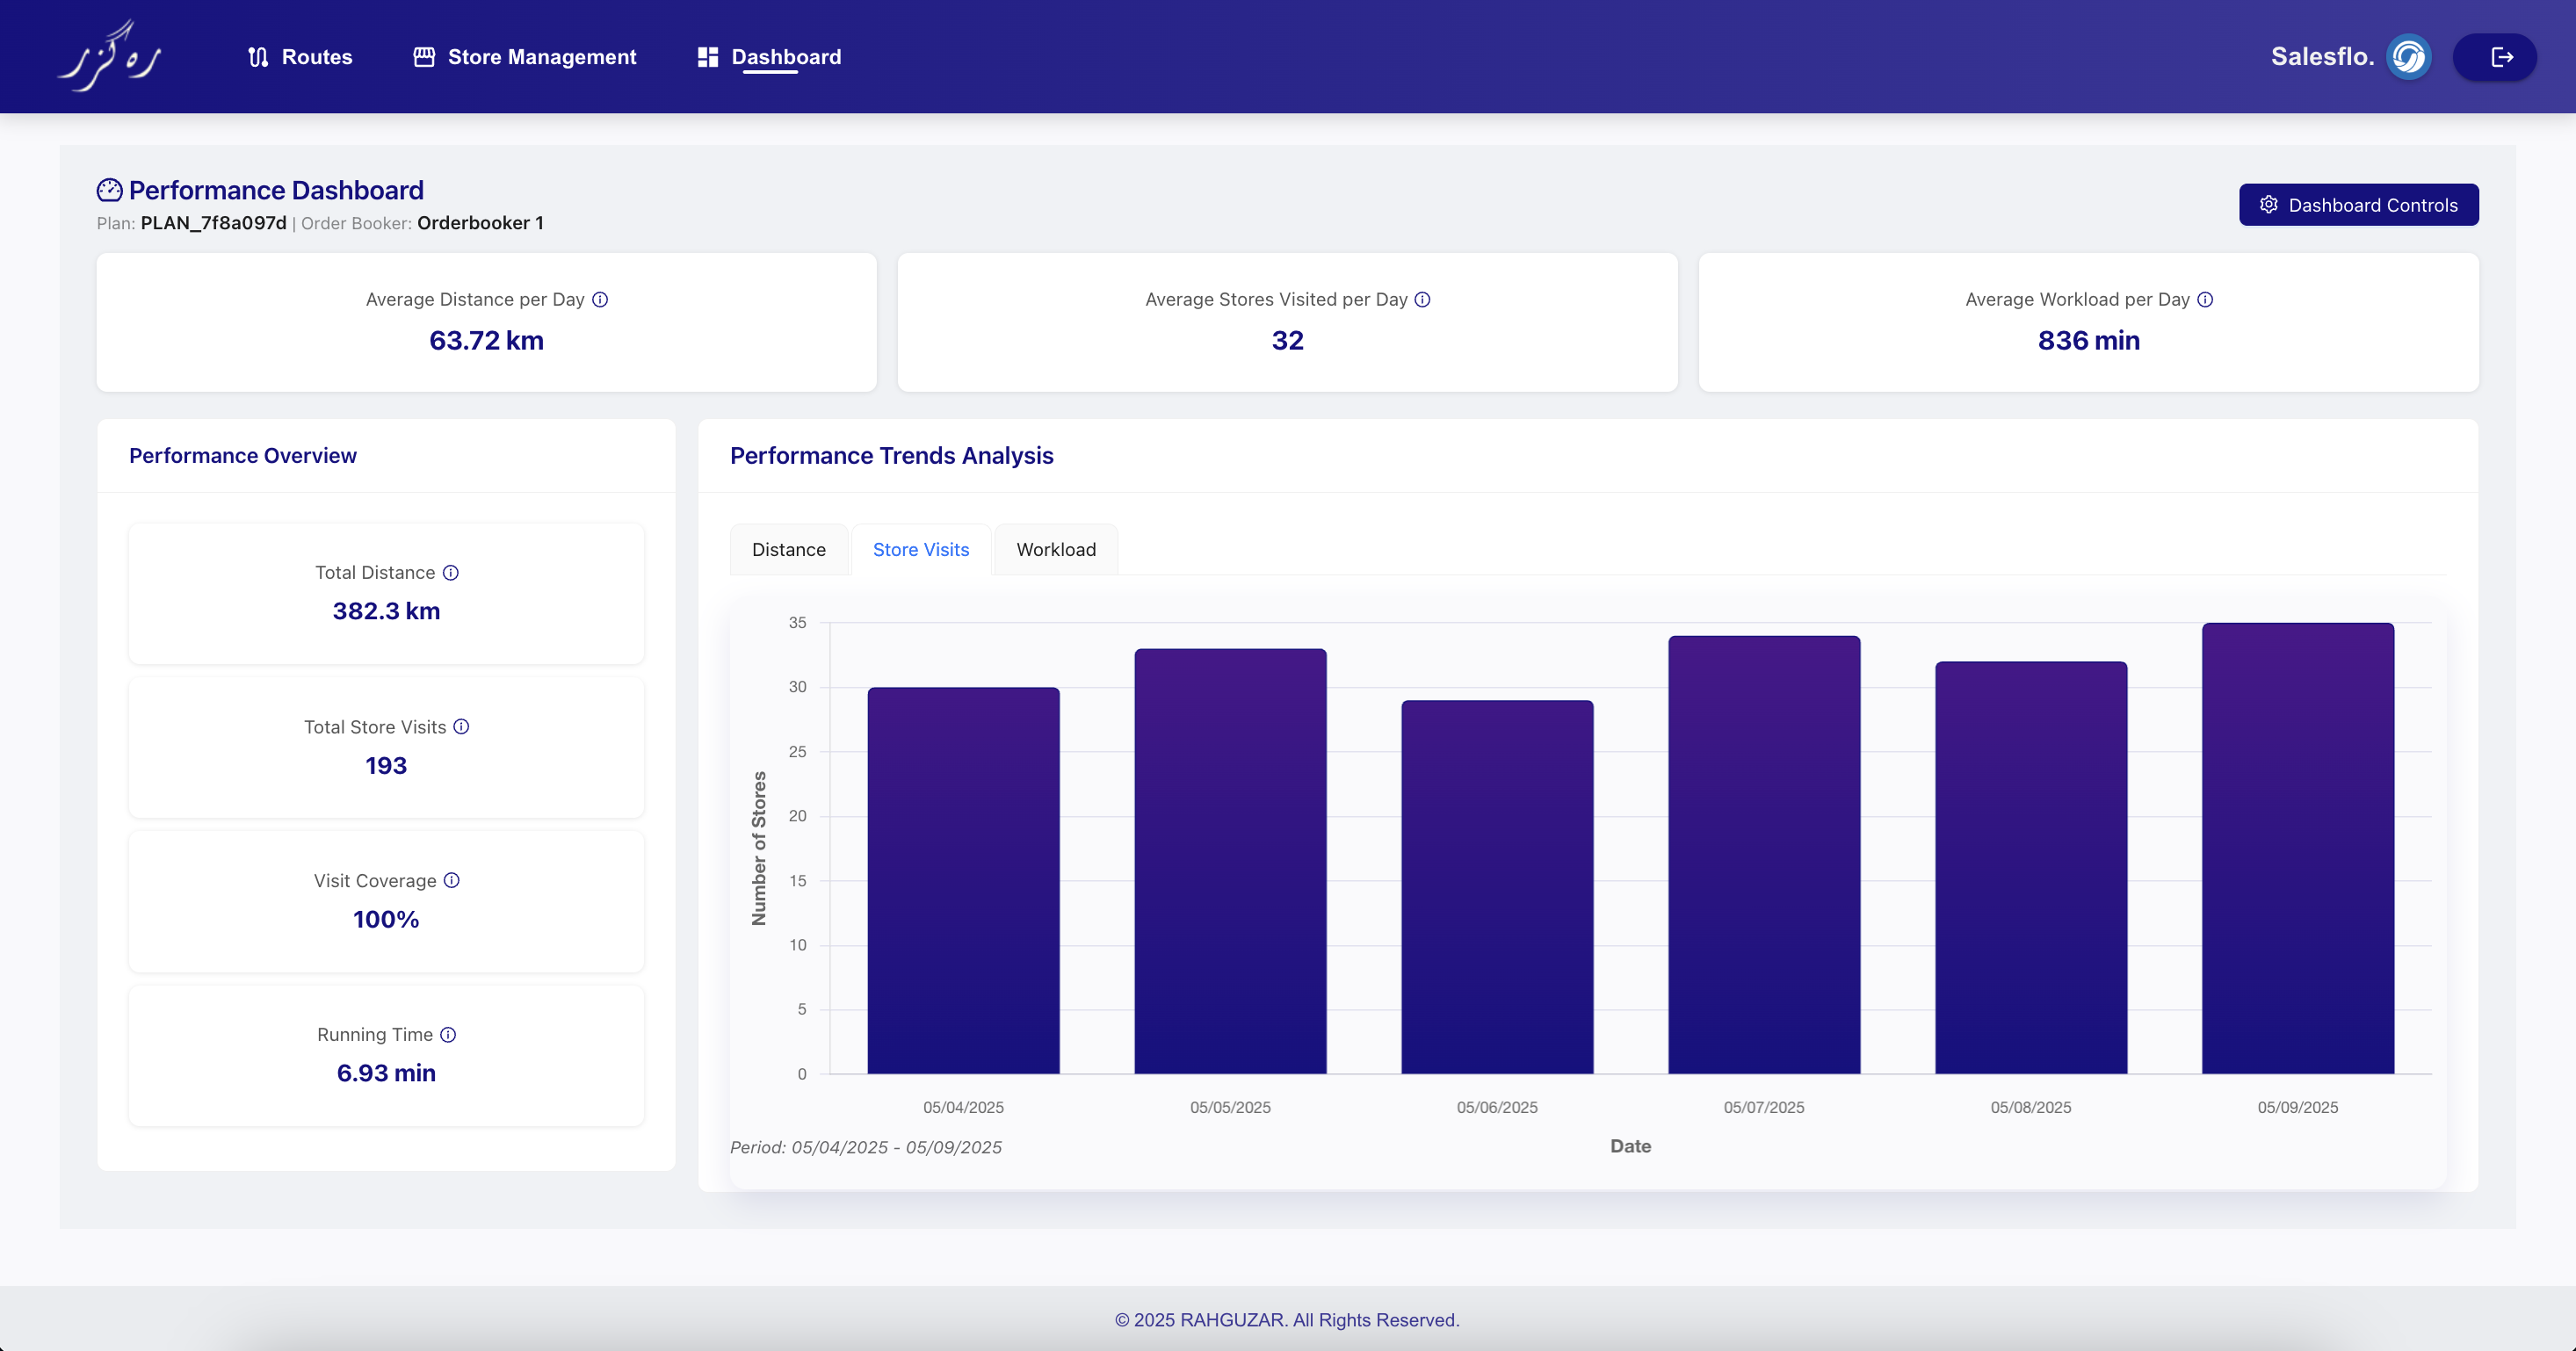
\includegraphics[width=1\textwidth]{images/dashboard.png} % Adjust width as needed
    \caption{Dashboard Page}
    \label{fig:image7}
\end{figure}
The ``Dashboard" screen is shown in Figure~\ref{fig:image7}. In this screen, the manager will be able to view certain KPIs that indicate the overall performance of the routes such as Average Daily Distance and Workload per Representative, Average travel time per per orderbooker or over all orderbookers. 

\subsection{Application Program Interface (API)}
The API layer is the backbone of the Rahguzar system, enabling seamless communication between the frontend, backend, and external services. Designed using REST principles, the API ensures efficient data exchange, operational scalability, and secure access control.

\subsubsection{REST API Endpoints}
The system is built with RESTful API endpoints that manage data transfer between components. Key endpoints include:

\begin{itemize}
    \item \textbf{Route Management Endpoints:}
    \begin{itemize}
        \item \texttt{POST /optimize} — Submits parameters to generate optimized journey plans.
        \item \texttt{POST /reroute-clusters} — Dynamically reassigns stores and reroutes OBs.
        \item \texttt{GET /get\_routes} — Retrieves finalized optimized routes.
    \end{itemize}

    \item \textbf{Store Profile Endpoints:}
    \begin{itemize}
        \item \texttt{GET /api/stores} — Fetches all store profiles.
        \item \texttt{POST /assign\_store} — Assigns a store to an order booker.
        \item \texttt{PUT /api/stores/\{store\_id\}} — Updates metadata of a specific store.
    \end{itemize}

    \item \textbf{Dashboard and KPI Endpoints:}
    \begin{itemize}
        \item \texttt{GET /get\_kpi\_data} — Returns key performance indicators.
        \item \texttt{GET /get\_graph\_data} — Fetches time-series analytics for visualization.
    \end{itemize}
\end{itemize}

\subsubsection{Authentication and Authorization}
To secure API access, the Rahguzar system employs JWT (JSON Web Tokens) for user authentication.

\begin{itemize}
    \item \texttt{POST /login} — Authenticates user credentials and returns a JWT token.
    \item \textbf{Token Usage:} The JWT token must be attached to the \texttt{Authorization} header as \texttt{Bearer <token>} in all subsequent API requests.
\end{itemize}

\subsubsection{External Services Integration}
To support essential routing and mapping functionalities, the system integrates with third-party services:

\begin{itemize}
    \item \textbf{Open Source Routing Machine (OSRM):}
    \begin{itemize}
        \item Dockerized and hosted on an EC2 instance for internal routing.
        \item \textbf{Endpoint:} \texttt{GET /route/v1/driving/\{lon,lat;lon,lat,...\}} — Returns route geometry and travel metadata in GeoJSON format.
    \end{itemize}
\end{itemize}

\subsubsection{Route Optimization Engine}
The route optimization component is embedded in the backend, using hybrid algorithms for clustering, scheduling, and routing.

\begin{itemize}
    \item \textbf{Python + OR-Tools:} Implements clustering, scheduling and route generation logic using Evolutionary Algorithms and TSP solvers.
\end{itemize}

\subsubsection{Data Storage and Synchronization}
The system utilizes a relational data model hosted on AWS RDS using PostgreSQL.

\begin{itemize}
    \item \textbf{PostgreSQL (via RDS):} Stores all persistent data including users, stores, routes, plans, and KPI metrics.
    \item \textbf{Synchronization Mechanisms:} Data flows between backend modules and frontend views are synchronized via well-defined API transactions and database-level consistency checks.
\end{itemize}

\subsubsection{Data Monitoring}
To enable effective monitoring, the API supports data updates and performance tracking:

\begin{itemize}
    \item \textbf{Performance Analytics:} Endpoints such as \texttt{/get\_kpi\_data} and \texttt{/get\_graph\_data} provide real-time insights on route efficiency, travel time, visit compliance, workload distribution, and other KPIs to support ongoing performance tuning and planning.
\end{itemize}



\subsection{Hardware/Communication Interfaces}
Our System relies on specific hardware and communication protocols to ensure seamless operation and efficient data management.

\subsubsection{Client-Side Hardware Requirements}
Manager Workstations: Managers access the system through web browsers on desktops or laptops for route planning and monitoring. Recommended specifications include:
\begin{itemize}
    \item \textbf{Processor:} Dual-core or higher.
    \item \textbf{RAM:} 4GB minimum.
    \item \textbf{Internet Connection:} Stable broadband with at least 5 Mbps for real-time data processing.
    \item \textbf{Browser Compatibility:} Supports modern web browsers like Chrome, Firefox, and Edge.
\end{itemize}

\subsubsection{Server-Side Infrastructure}
The backend and database components are hosted on cloud infrastructure (AWS) to ensure availability, fault tolerance, and scalability.

\begin{itemize}
    \item \textbf{Application Server (EC2):}
    \begin{itemize}
        \item Hosted on an Amazon EC2 instance (e.g., t3.medium or higher).
        \item Runs the Flask-based backend application, route optimization engine, and API endpoints.
        \item Configured with Gunicorn and optionally Nginx for request handling and reverse proxy.
        \item Operating System: Ubuntu Server 20.04 LTS or equivalent.
    \end{itemize}

    \item \textbf{Database Server (RDS):}
    \begin{itemize}
        \item PostgreSQL instance managed via Amazon RDS.
        \item Stores all system data including user credentials, store metadata, plan configurations, route outputs, and KPI records.
        \item SSD-based storage with automated backup and optional multi-AZ redundancy.
    \end{itemize}

    \item \textbf{Storage:} EC2 instance uses SSD storage for intermediate computation results and application logs.

    \item \textbf{Networking:} Secured via AWS security groups. Backend accessible via HTTPS; database accessible only through private IPs or controlled access rules.
\end{itemize}

\subsubsection{Communication Interfaces}
\begin{itemize}
    \item \textbf{Internet Connection:} All interactions between the frontend and backend rely on a stable internet connection for data synchronization and API requests.
\newpage
    \item \textbf{Data Communication Protocols:}
    \begin{itemize}
        \item \textbf{HTTPS:} Secure communication between frontend, backend, and external services like Google Maps API.
        \item \textbf{API Calls:} RESTful API requests enable data transfer for route management, visit updates, and user authentication.
    \end{itemize}
\end{itemize}

\subsubsection{Routing Service (Dockerized OSRM)}
The system utilizes a containerized instance of the Open Source Routing Machine (OSRM) to compute real-world travel distances and generate accurate road-based routes.

\begin{itemize}
    \item \textbf{Deployment Method:} OSRM is deployed via Docker on an EC2 instance to ensure isolation, portability, and ease of deployment.
    \item \textbf{Routing Backend:} Based on preprocessed OpenStreetMap data using the `osrm-backend` image.
    \item \textbf{Port Configuration:} Accessible via HTTP on port 5002 internally, secured behind firewall rules.
    \item \textbf{Container Runtime:} Docker Engine on Ubuntu Server.
    \item \textbf{Data Source:} OSM PBF file for the region of operation (e.g., Pakistan or selected city).
    \item \textbf{Use Case Integration:} Accessed by the backend during route optimization to compute driving distances between stores.
\end{itemize}



\section{Use Cases}
\begin{itemize}
    \item \textbf{User Authentication and Access Control}
    \begin{itemize}
        \item \textbf{Description:} Ensure secure access to the system for both managers and field staff.
        \item \textbf{Actions:}
        \begin{itemize}
            \item As a manager, I want to log in securely to access my dashboard and create journey plans.
            \item As the system, I need to authenticate users to ensure only authorized managers and field staff access the application.
        \end{itemize}
    \end{itemize}
    
    \item \textbf{Route Plan Creation, Configuration, and Optimization}
    \begin{itemize}
        \item \textbf{Description:} Enable the creation of optimized routes based on configurable parameters.
        \item \textbf{Actions:}
        \begin{itemize}
            \item As a manager, I want to create a new optimized route for my field team, configuring parameters like shift timings and visit frequency to align with operational requirements.
            \item As the system, I need to generate optimized routes using parameters such as shift times, visit frequencies, and priorities, ensuring efficient route suggestions for managers.
        \end{itemize}
    \end{itemize}

    \item \textbf{Plan Generation}
    \begin{itemize}
        \item \textbf{Description:} Generate long-term journey plans based on store visit requirements.
        \item \textbf{Actions:}
        \begin{itemize}
            \item As a manager, I want the ability to generate custom day journey plans, providing my team with a consistent schedule for store visits.
            \item As the system, I need to automatically generate journey plans for custom day schedules based on specified visit frequencies.
        \end{itemize}
    \end{itemize}
    
    \item \textbf{Dynamic Rerouting and Manual Overrides}
    \begin{itemize}
        \item \textbf{Description:} Allow for real-time adjustments to routes, either dynamically by the system or manually by the manager.
        \item \textbf{Actions:}
        \begin{itemize}
            \item As a manager, I want to make manual adjustments to routes to adapt to urgent needs or unexpected changes.
            \item As a manager, I want the system to dynamically reroute based on parameter changes after the route is generated.
            \item As the system, I need to recalculate routes dynamically if the manager makes changes to parameters, ensuring updated routes without disrupting existing operations.
        \end{itemize}
    \end{itemize}
    
    \item \textbf{Route Sharing and Export}
    \begin{itemize}
        \item \textbf{Description:} Facilitate the sharing of finalized routes with field staff.
        \item \textbf{Actions:}
        \begin{itemize}
            \item As a manager, I want to export and share finalized routes with field staff so they have clear guidance on their daily tasks and destinations.
            \item As the system, I need to support data export so that managers can download route plans and reports for offline access if needed.
        \end{itemize}
    \end{itemize}
    
    \item \textbf{Store Profile Integration and Viewing}
    \begin{itemize}
        \item \textbf{Description:} Provide access to detailed store profiles to aid in route planning.
        \item \textbf{Actions:}
        \begin{itemize}
            \item As a manager, I want to view detailed store profiles, including location and sales channel, to prioritize visits and plan routes effectively.
            \item As the system, I need to integrate and maintain comprehensive store profiles, making it easier for managers to access relevant data during route planning.
        \end{itemize}
    \end{itemize}
    
    \item \textbf{Interactive Map Visualization}
    \begin{itemize}
        \item \textbf{Description:} Enable map-based visualization of routes and store locations.
        \item \textbf{Actions:}
        \begin{itemize}
            \item As a manager, I want to see routes on an interactive map, allowing me to visualize store locations and make adjustments as needed.
            \item As the system, I need to display routes and navigation data on an interactive map interface for both managers and field staff.
        \end{itemize}
    \end{itemize}
    
    \item \textbf{Performance Tracking and KPI Monitoring}
    \begin{itemize}
        \item \textbf{Description:} Track and analyse performance metrics to evaluate route effectiveness.
        \item \textbf{Actions:}
        \begin{itemize}
            \item As a manager, I want to track KPIs like travel time and visit completion rates to assess route performance and make improvements.
            \item As the system, I need to automate KPI tracking (e.g., average travel time, total distance, workload) to provide ongoing insights without requiring manual input from managers.
        \end{itemize}
    \end{itemize}
    
    \item \textbf{System Data Synchronization}
    \begin{itemize}
        \item \textbf{Description:} Sync store and route data to ensure accurate and up-to-date information.
        \item \textbf{Actions:}
        \begin{itemize}
            \item As a manager, I want the system to view store information and modify store statuses, giving me reliable data for decision-making.
            \item As the system, I need to synchronize with external databases to maintain current and accurate store and route data for all users.
        \end{itemize}
    \end{itemize}
    

    
\end{itemize}

\begin{center}

    \begin{figure}[H]
        \centering
        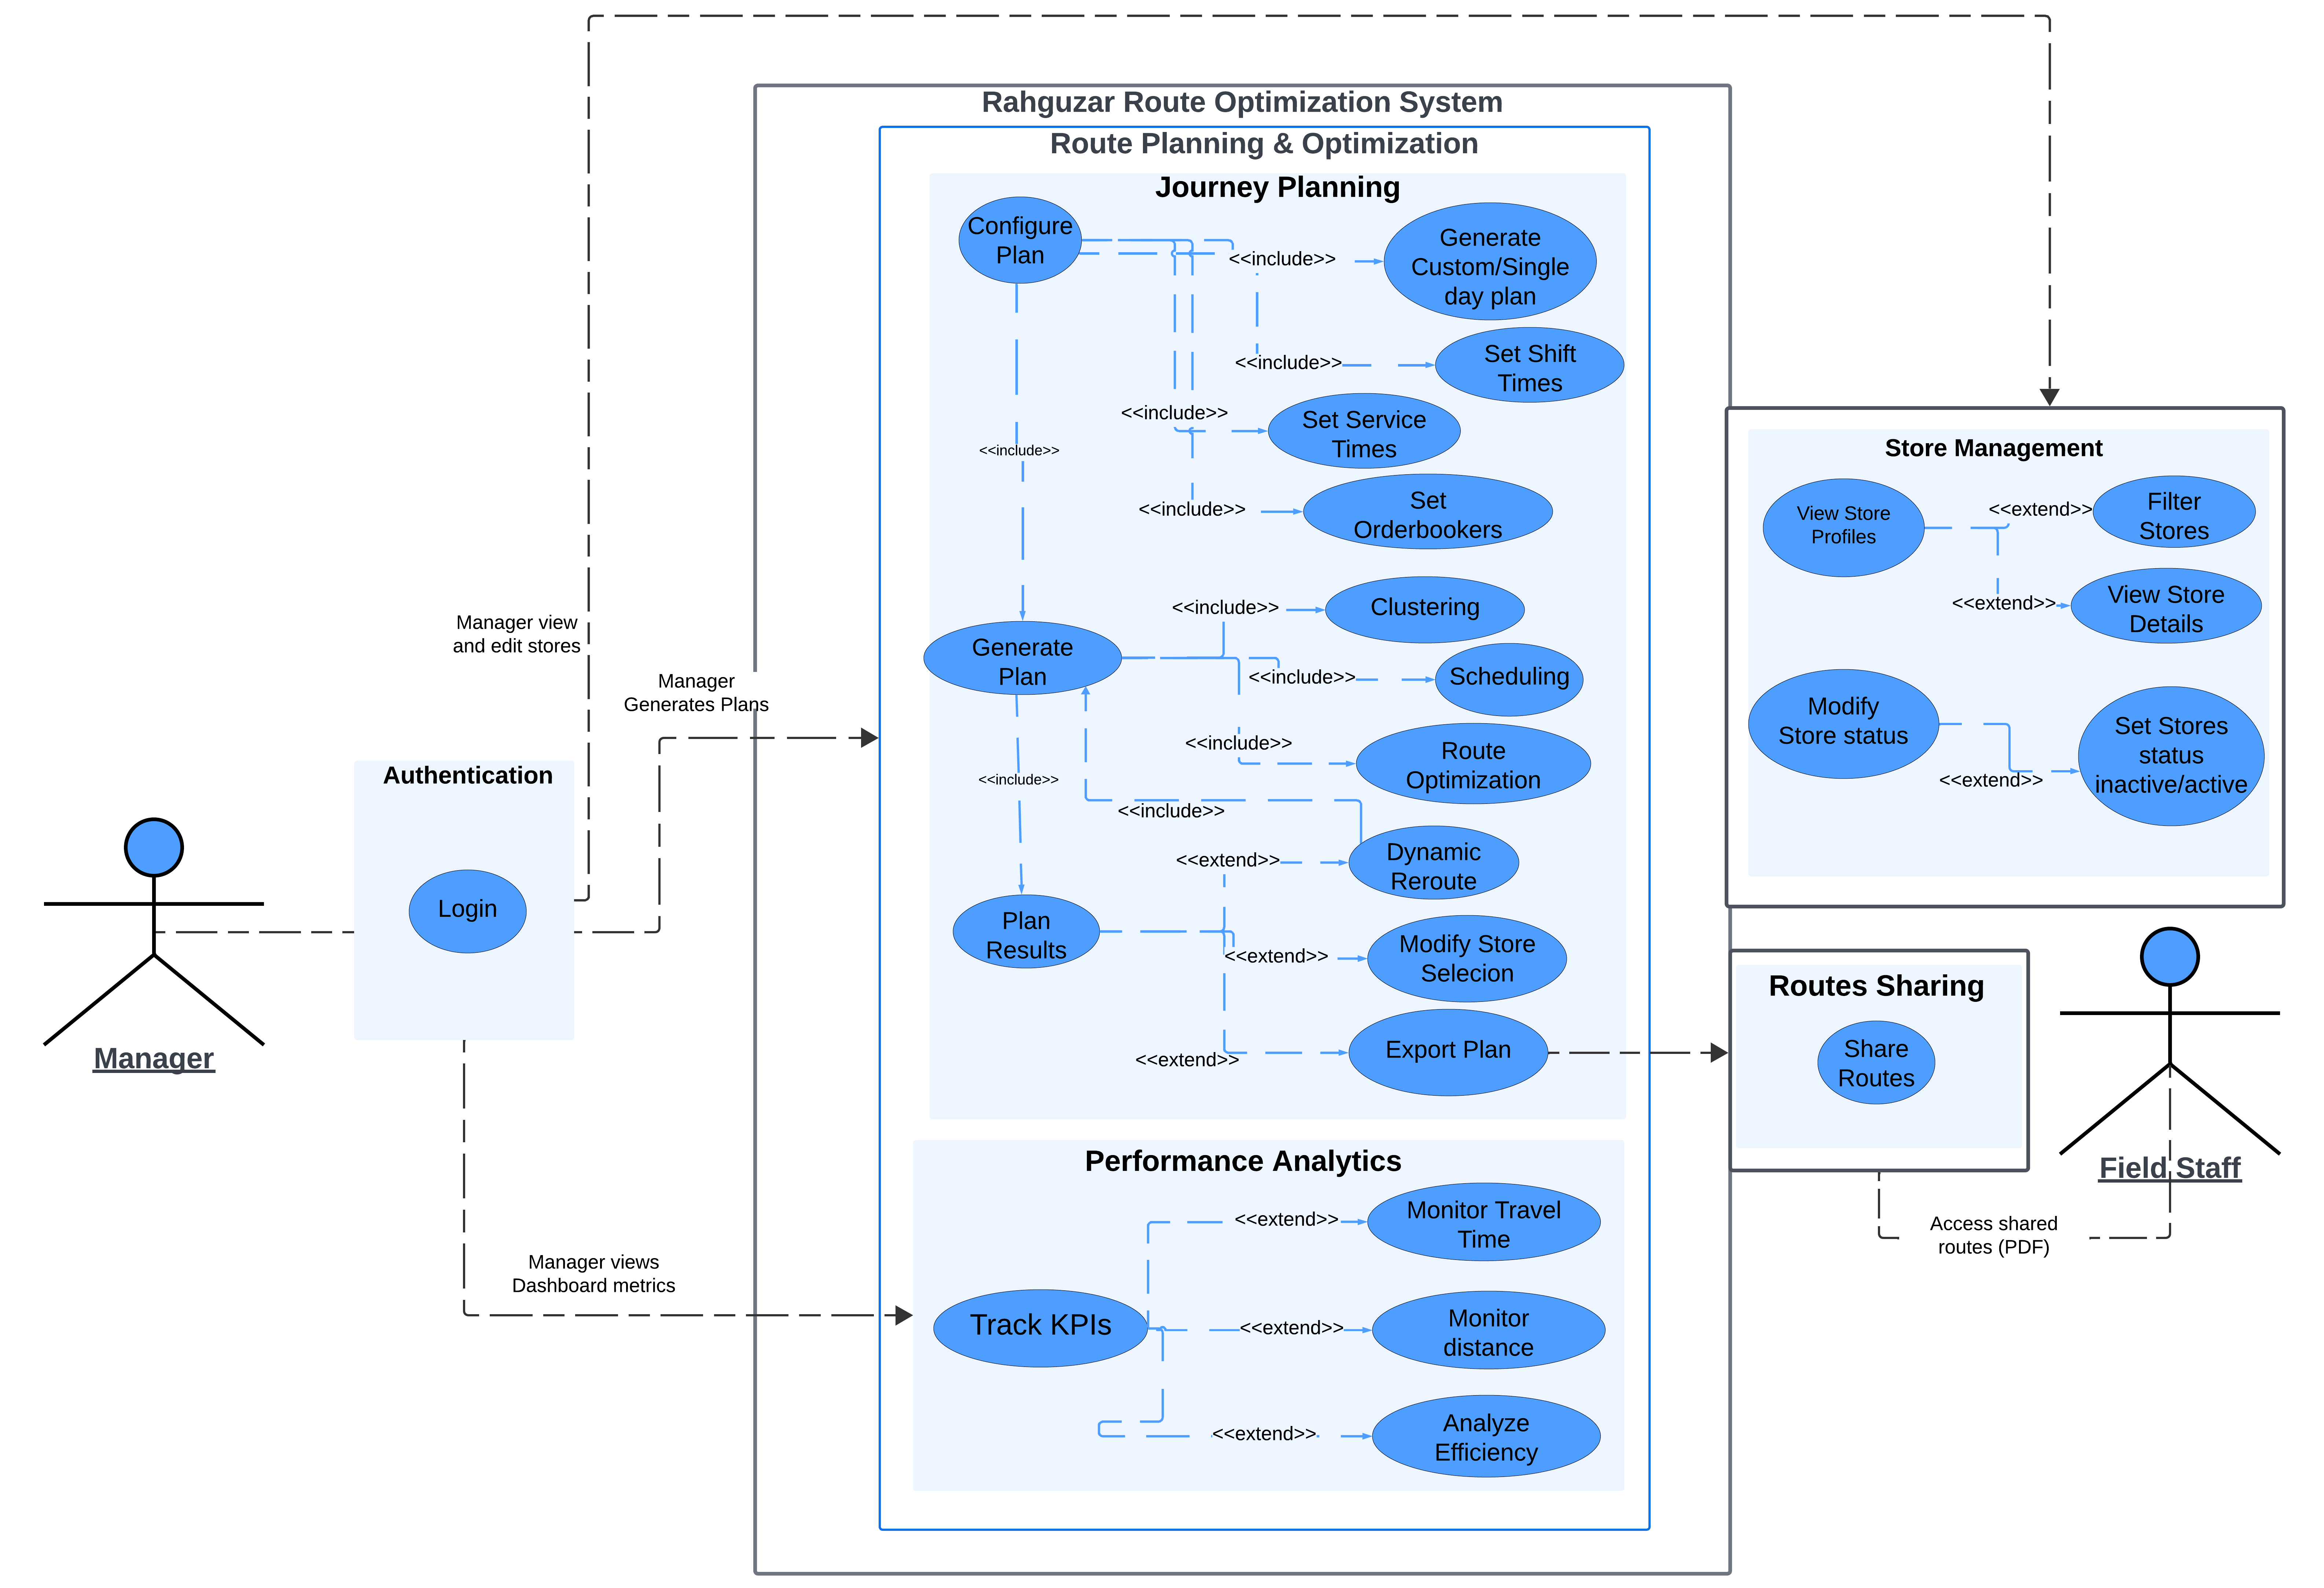
\includegraphics[width=0.98\textwidth]{images/Rahguzar - Use Case - Core System.png} 
        \caption{Rahguzar's Use Case Diagram}
    \end{figure}
\end{center}

\section{Datasets}
% This section describes the specific dataset(s) used to build our system. An appropriate snapshot of the dataset(s) is also included. Futher details, when needed, are presented in the appendix.
This section outlines the primary datasets that will support Rahguzar’s intelligent route planning and scheduling functionalities. These datasets provide crucial information on stores, visits, journey plans, and operational factors essential for optimized route generation. As per the NDA with SalesFlo, we are not permitted to share or disclose the data provided to us. 
\subsection*{Overview of Datasets}

\begin{enumerate}

\item \textbf{Store Universe} \\
This dataset provides foundational information on each store, including location, operational status, and distributor associations. Key fields include:
    \begin{itemize}
        \item \textbf{storecode:} Unique identifier for each store.
        \item \textbf{storestatus:} Operational status (active or inactive).
        \item \textbf{latitude and longitude:} Geographic coordinates.
        \item \textbf{distributorcode:} Code for the distributor linked to the store.
        \item \textbf{pjpcode:} Code for the Permanent Journey Plan (PJP) associated with the store.
    \end{itemize}
This dataset is essential for determining which stores to include in routes based on location and operational status.

\item \textbf{Store Hierarchy} \\
This dataset offers classification and hierarchical details, allowing route customization based on store attributes such as region or sales channel. Key fields include:
    \begin{itemize}
        \item \textbf{storecode:} Identifier for each store.
        \item \textbf{areatype, townid, localityid:} Geographical identifiers.
        \item \textbf{channeltypeid and channelid:} Sales channel identifiers (e.g., retail, wholesale).
        \item \textbf{storeclassificationIDs: } These classification IDs will be used to further distinguish between certain store categories.
    \end{itemize}
This data enables Rahguzar to organize routes by region and sales channel, optimizing for specific geographic and operational criteria.

\item \textbf{Visits} \\
The Visits dataset records historical visit information for each store, including time spent, visit order, and outcomes. Key fields include:
    \begin{itemize}
        \item \textbf{visitid:} Unique identifier for each visit.
        \item \textbf{pjpcode:} Journey plan code associated with the visit.
        \item \textbf{visitdate, visitstarttime, visitendtime:} Time data for analyzing visit durations.
        \item \textbf{visitspenttimeinseconds:} Total time spent at the store during the visit.
        \item \textbf{orderstatus:} Status of any order placed during the visit.
        \item \textbf{visiststatus: } Status determining if a visit has been completed or not.
        \item \textbf{syncdown, syncup, syncdowndatetime: } These fields track the synchronization status and timing of visit records: syncdown shows if data was downloaded to the device, syncup if it was uploaded to the server, and syncdowndatetime logs the last download timestamp.
    \end{itemize}
This dataset supports route optimization by providing insights into visit frequency and duration, refining future scheduling.

\end{enumerate}

% \subsection*{Additional Datasets Needed}

% To enhance Rahguzar's functionality, the following additional datasets may be required:

% \begin{enumerate}

% \item \textbf{Order Booker Shifts Dataset} \\
% This dataset contains information on the availability and shifts of order bookers. Key fields include:
%     \begin{itemize}
%         \item \textbf{bookerid:} Unique identifier for each order booker.
%         \item \textbf{shiftstarttime and shiftendtime:} Start and end times of each shift.
%         \item \textbf{availabilitystatus:} Indicates whether the booker is available or unavailable.
%     \end{itemize}
% This dataset is essential for scheduling routes within the working hours of each order booker, optimizing route generation according to workforce availability.

% \item \textbf{Geographic Data} \\
% Geographic and road network data provide detailed map and routing information, potentially sourced via the Google Maps API or GIS data services. Key components include:
%     \begin{itemize}
%         \item \textbf{roadnetwork:} Map of roads, including distances and travel times.
%         \item \textbf{trafficpatterns:} Historical traffic data for congestion analysis.
%         \item \textbf{geofencingdata:} Predefined boundaries for specific zones, regions, or territories.
%     \end{itemize}
% This dataset enables precise route calculations, factoring in real-time or historical traffic conditions to minimize travel time.

% \item \textbf{Store Activity Requirements} \\
% This dataset details the specific activities and time requirements for each store visit, allowing Rahguzar to optimize for different tasks performed at each store. Key fields include:
%     \begin{itemize}
%         \item \textbf{storecode:} Identifier for each store.
%         \item \textbf{activitytype:} Type of activity required (e.g., stock check, merchandising).
%         \item \textbf{estimatedtime:} Average time required to complete each activity.
%     \end{itemize}
% This dataset supports the system’s ability to tailor visit durations based on store requirements, leading to more accurate time estimates for each route.
% \end{enumerate}

\subsection*{Data Utilization in Rahguzar}

Together, these datasets will support Rahguzar’s core functionalities, including:
\begin{itemize}
    \item \textbf{Efficient Route Planning:} Leveraging store locations, operational statuses, and road networks for optimal routing.
    % \item \textbf{Dynamic Scheduling:} Using order booker shifts and activity requirements to generate flexible schedules aligned with store needs and workforce availability.
    \item \textbf{Traffic and Geographic Optimization:} Utilizing geographic data to plan routes that avoid congestion and optimize for specific zones or territories.
    % \item \textbf{Geographical Filtering:} Geographical and channel-based categorization from the Store Hierarchy dataset will help managers plan routes tailored to specific regions and sales priorities.
    \item \textbf{Route Efficiency Analysis:} The Visits dataset will provide insights into average visit durations and travel times, which will inform the route optimization algorithm and support KPI tracking for system performance.
\end{itemize}


\section{System Diagram}
\begin{center}
        \begin{figure}[H]
        \centering
        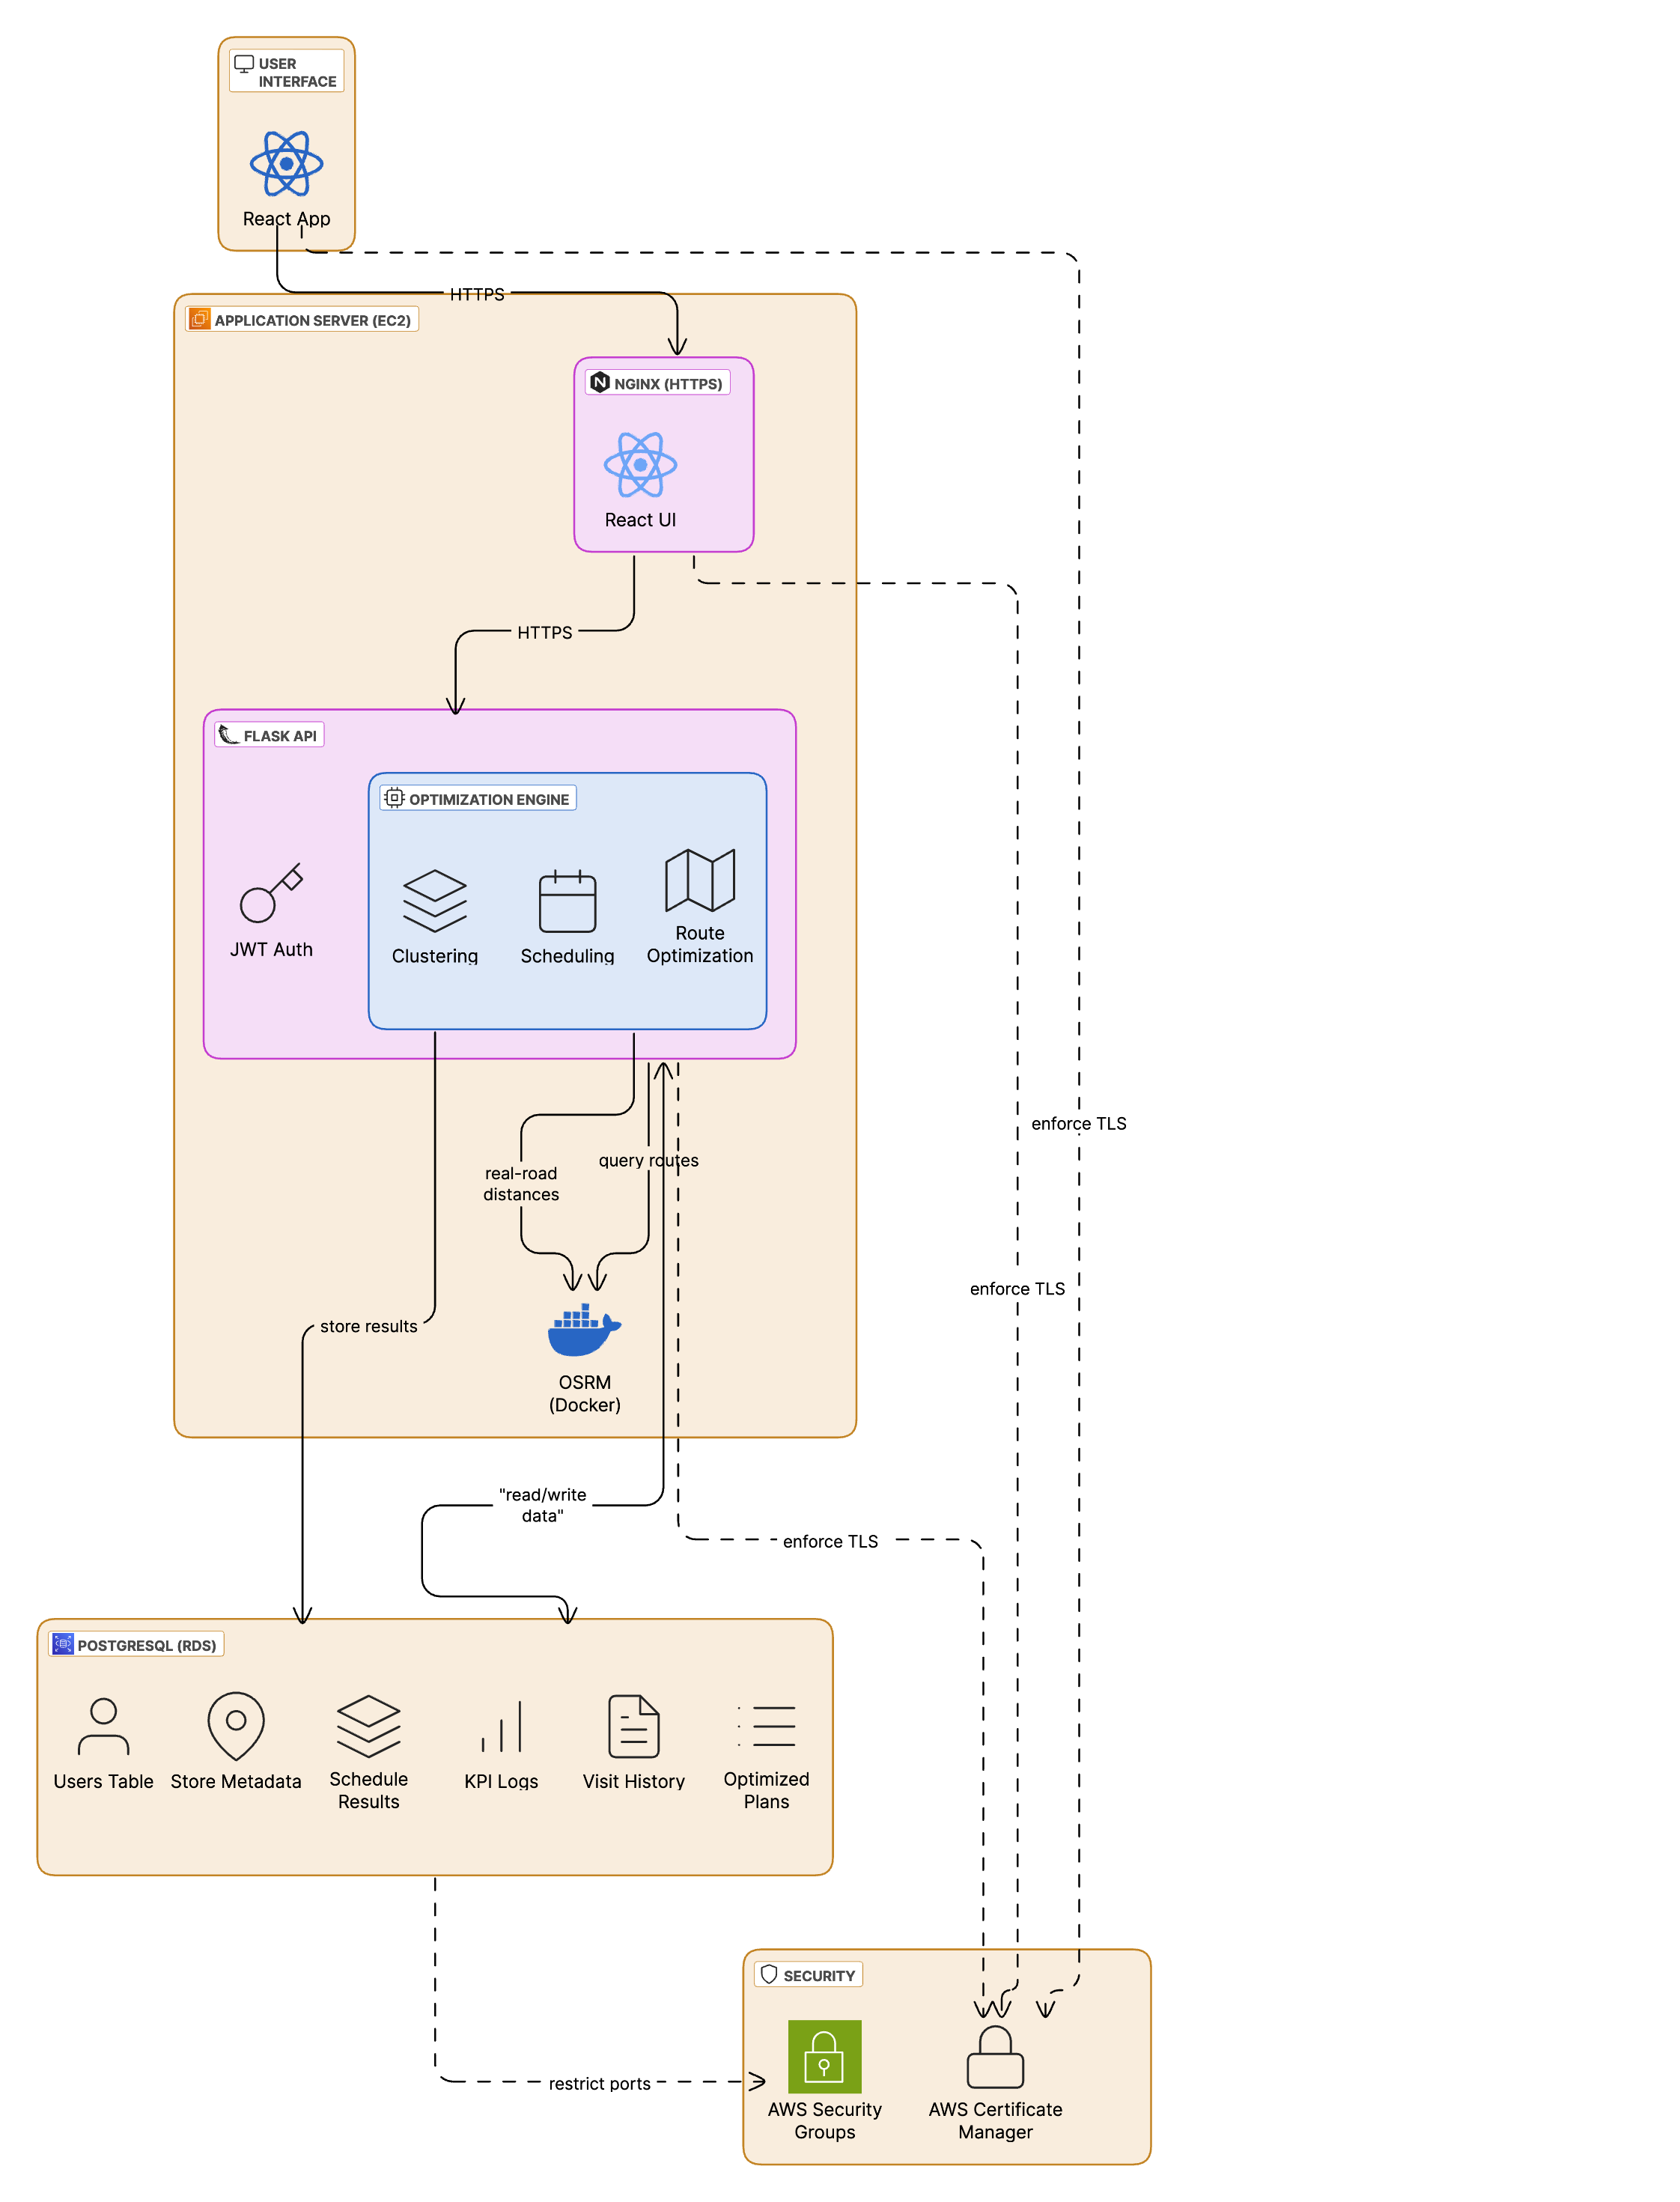
\includegraphics[width=\textwidth, height=0.75\textheight]{images/diagram.png} 
        \caption{Rahguzar's System Architecture Diagram}
    \end{figure}
\end{center}

\chapter{Software Design Specification (SDS)}
\label{chap:sds}
The Software Design Specifications outlines the key design components of the Rahguzar system, including its software architecture, database schema, and core optimization logic.

\section{Software Design}

% This section presents the UML class diagram and gives a brief description of each class in our system. Attributes and methods of each class and relationship among classes are clearly presented.

\begin{figure}[H]
    \centering
    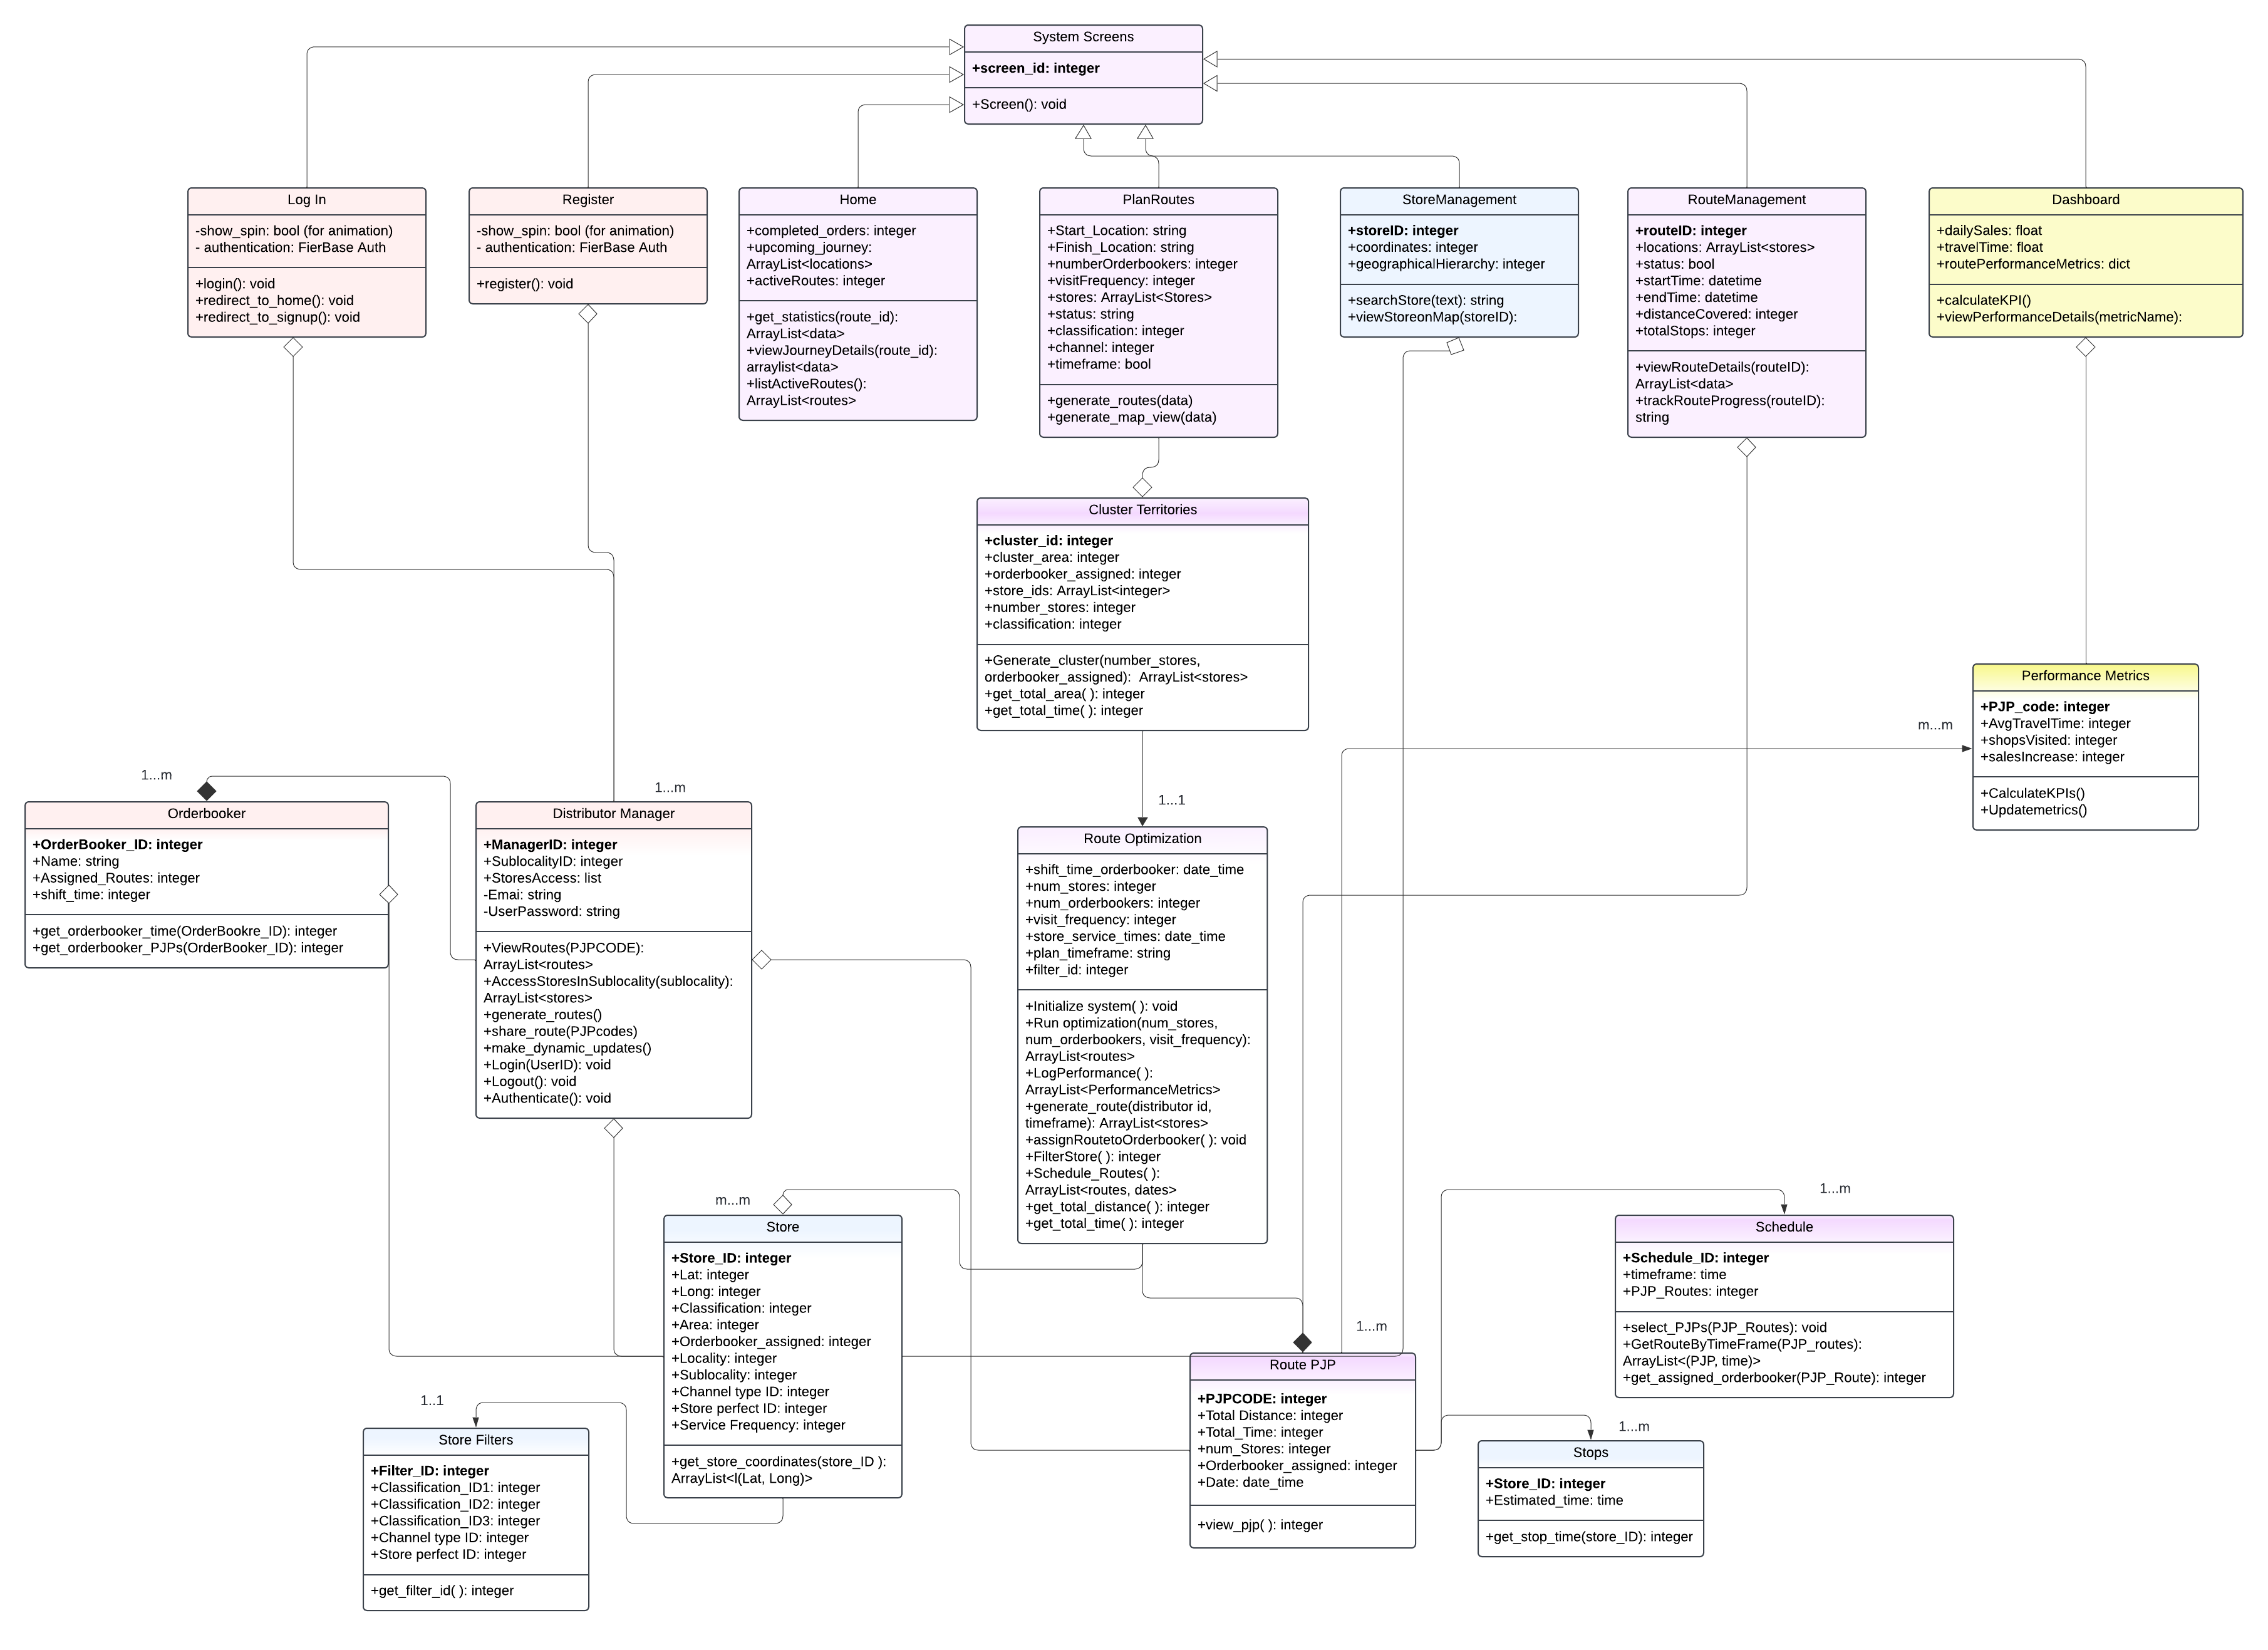
\includegraphics[width=0.9\textwidth]{images/UML class f2.png} % Adjust the width as needed
    \caption{UML Class Diagram}
    \label{fig:UML-image}
\end{figure}

% Your report will contain ONE of the following 2 sections.

As shown in Figure~\ref{fig:UML-image}, the UML diagram starts off by showing the screens that are connected to the system. The Register screen creates the object for the distributor manager, giving them access to the system and screens mentioned such as home, plan routes, route management, and etc. Next, the user has the option to Plan Routes from that screen where they give certain parameters mentioned in the attributes. This creates a cluster object for different areas containing different stores. Next, the optimal PJP route will be determined in each cluster that creates the object for clusters. After this, the stores in each cluster will be connected to form a route, creating a routes class that is the optimal PJP plan. These routes can also be viewed on a schedule view to visually analyze how the upcoming PJPs look like. Moreover, a separate stores table is connected to the child table of stores filters that provides the further classification of each store id. Lastly, the dashboard screen gets the KPIs from the Performance Metrics class to display how the performance of each PJP is and to visualize it in graphs and display the metrics.

\section{Data Design}

This section presents the structure of our database that caters to persistent data storage in our project. The structure is shown as a normalized data model for relational databases. It clearly shows entities, attributes, relationships with their cardinalities, and primary and foreign keys. We have used Postgresql ERD to build our data model.

\begin{figure}[H]
    \centering
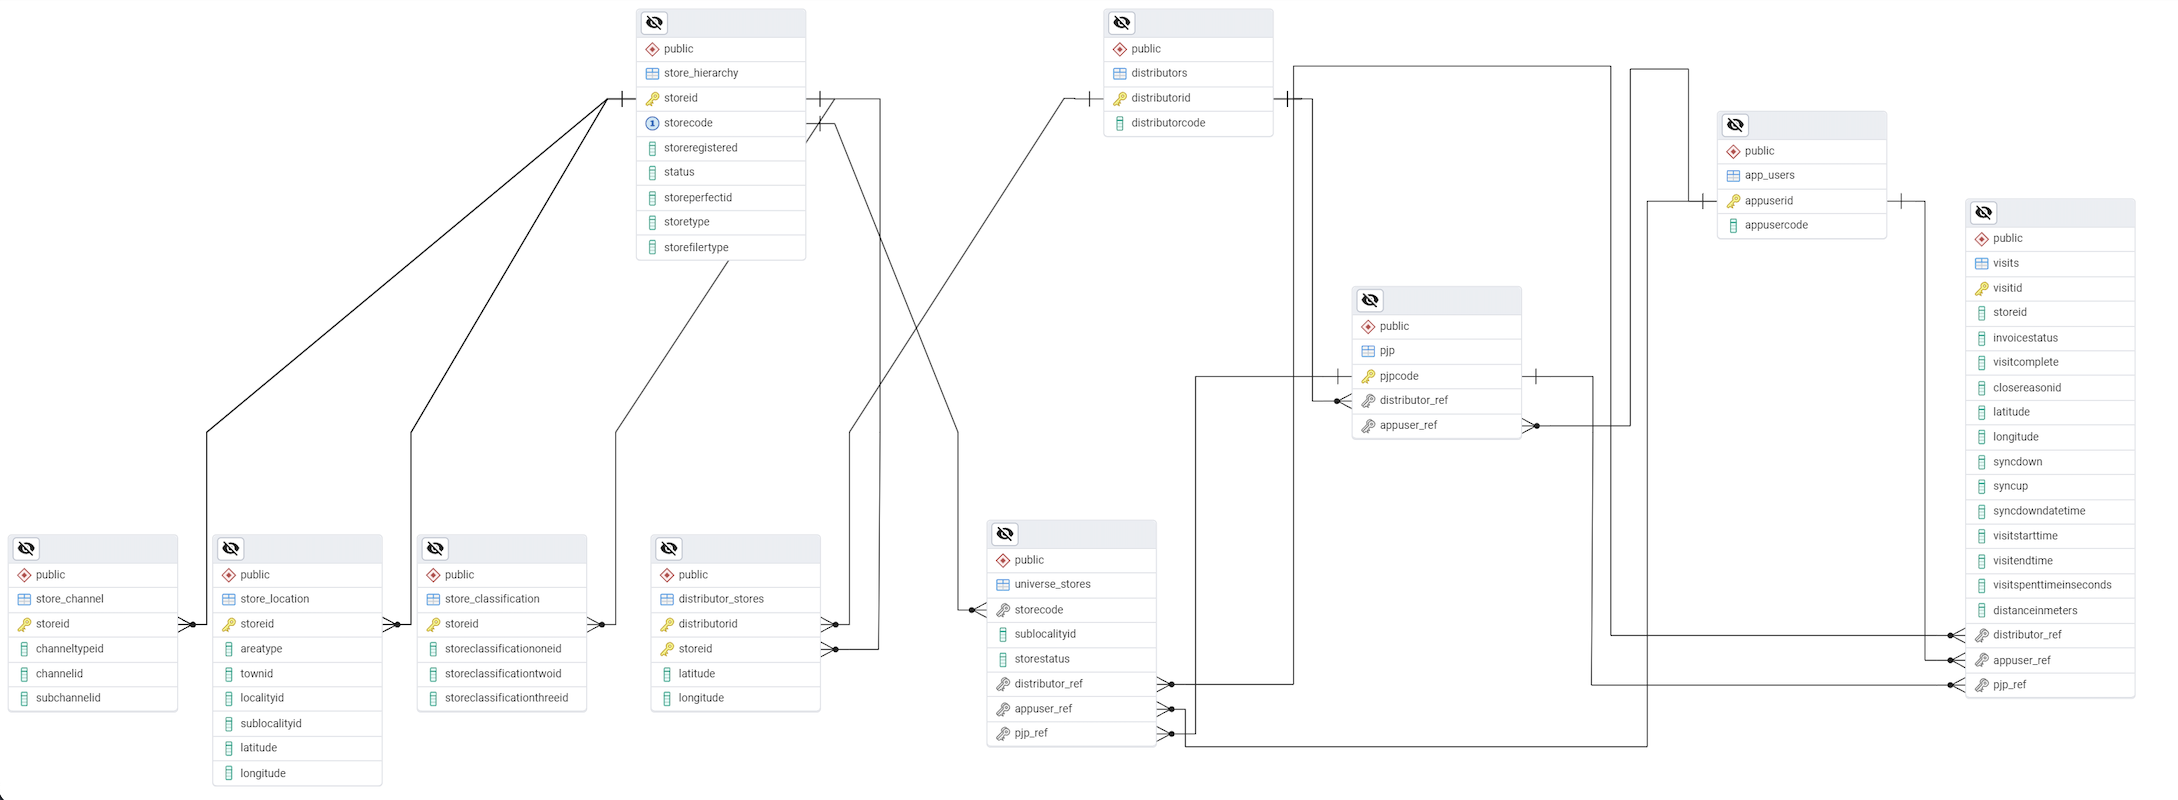
\includegraphics[width=\textwidth]{images/erd.png} % Adjust the width as needed
    \caption{ERD Diagram}
    \label{fig:UML-image}
\end{figure}
\begin{figure}[H]
    \centering
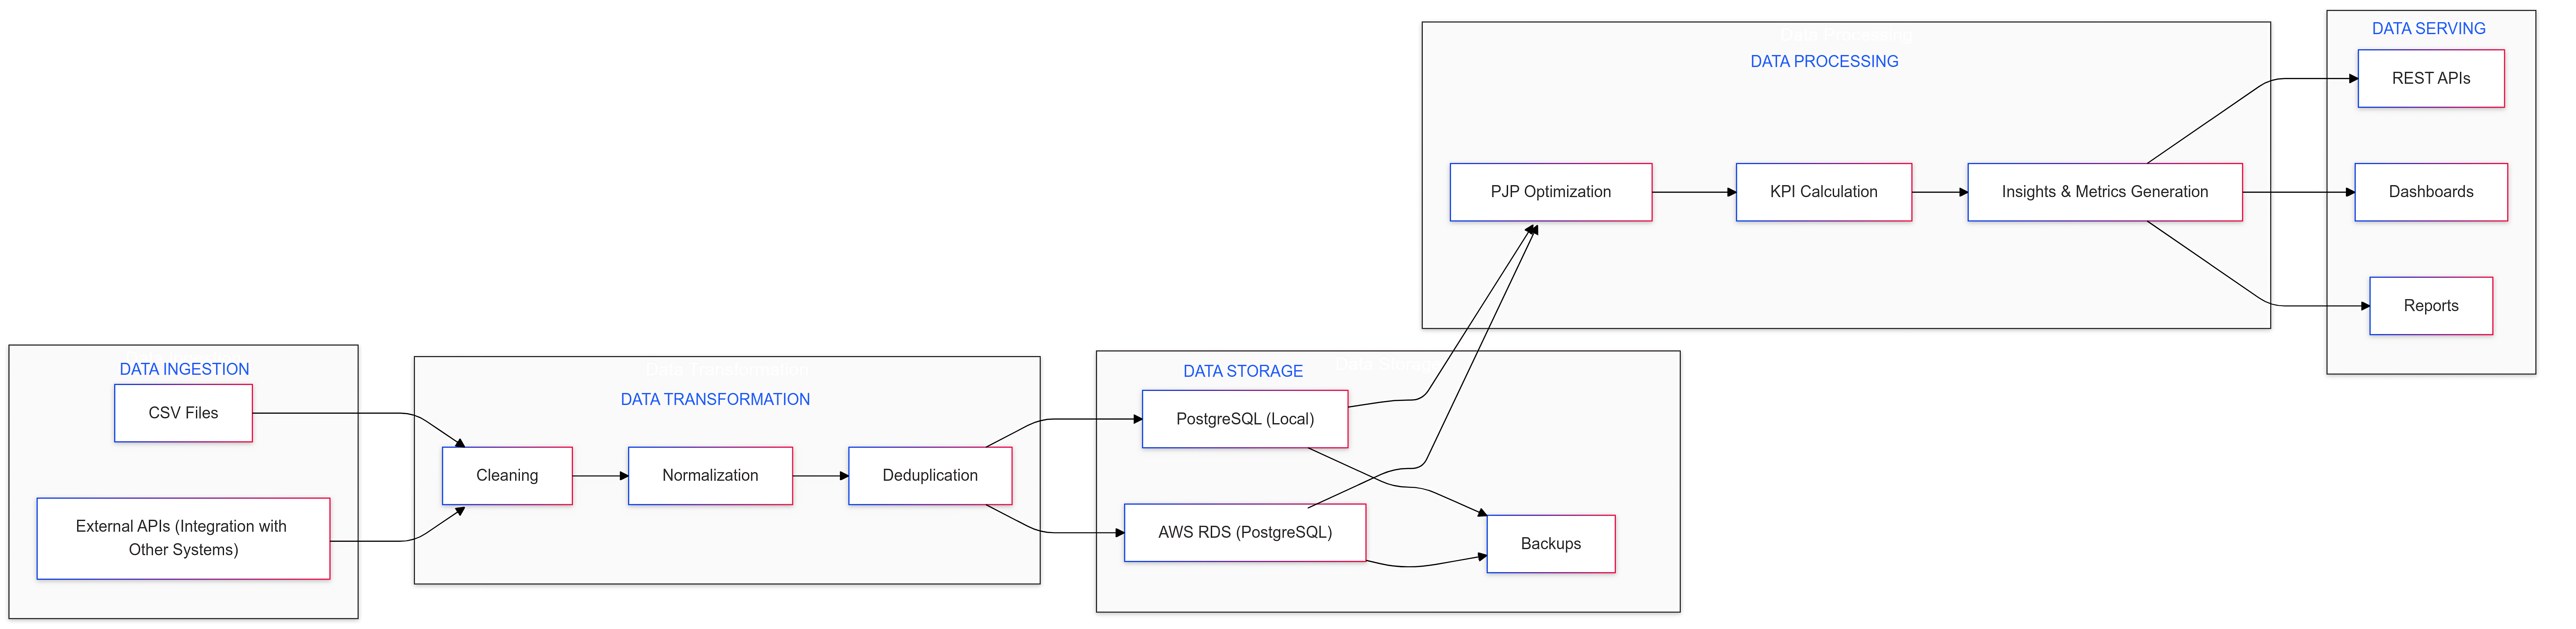
\includegraphics[width=1.1\textwidth]{images/DataPipeline (1).png} % Adjust the width as needed
    \caption{End-to-end data pipeline showcasing ingestion, transformation, storage, processing, and serving}
    \label{fig:UML-image}
\end{figure}

 
% \section{Technical Details}

% As shown above, our project includes an ERD created based on the cleaned data. Additionally, following are the technical aspects of the algorithm (Evolutionary Algorithm).
% \\
% The primary objectives of our algorithm are:
% \begin{itemize}
%     \item Maximizing the number of shops visited within the constraints.
%     \item Minimizing the total distance traveled to improve route efficiency.
%     \item Minimizing overall time spent, which includes travel and time spent at each store.
% \end{itemize}

% The constraints of our algorithm are:
% \begin{itemize}
%     \item \textbf{Number of order bookers}: Determines the workload distribution and affects route planning.
%     \item \textbf{Shift times}: Incorporates break times, holidays, and working hours.
%     \item \textbf{Duration at each store}: This is a fixed value for each visit and must be accounted for in total route time.
% \end{itemize}
% These objectives and constraints guide the design and functionality of our route optimization algorithm. The algorithm dynamically adapts to these parameters to give optimal route plans.

\section{Technical Details}

The Rahguzar system uses a multi-stage route optimization algorithm composed of clustering, scheduling, and routing. This pipeline ensures operational efficiency while adhering to business constraints such as working hours, visit frequencies, and travel limits.

\begin{itemize}
    \item \textbf{Clustering:} Stores are grouped based on geographic proximity using density- or centroid-based clustering.
    \item \textbf{Scheduling:} An Evolutionary Algorithm assigns stores to order bookers across a multi-day plan, optimizing workload balance and visit coverage.
    \item \textbf{Routing:} Store sequences are optimized using road-based routing with OSRM, minimizing total travel time and distance.
\end{itemize}
The algorithm aims to maximize shop visits, minimize total distance traveled, and reduce overall time, including both travel and in-store duration. It operates under key constraints such as the number of order bookers, shift timings, and fixed visit durations per store, ensuring realistic and efficient route plans.


The system supports dynamic rerouting, manual overrides, and constraint-based optimization to remain adaptive to real-world field operations. Full methodological details including algorithmic structure, fitness design, and tuning are provided in the Methodology section.


\chapter{Development}
\label{chap:dev}
\input{chapters/development}

\chapter{Methodology}
\label{chap:method}
\input{chapters/methodology}

\chapter{Experiments and Results}
\label{chap:results}
This chapter aims to present the results of the experiments conducted across Rahguzar’s clustering, scheduling, and routing phases to evaluate their impact on route optimization, workload balancing, and service coverage. Each algorithm was tested individually and as part of the integrated pipeline. Additionally, Rahguzar’s performance was benchmarked against Salesflo using real distributor datasets, comparing outcomes in terms of total travel distance, execution time, and overall planning efficiency.

\section{Algorithmic Phases and Experiment Results}

This section presents the methodology and results from a series of experiments conducted to determine the optimal combinations of algorithms for different phases of the optimization process.




\subsection{Phase 1: Hybrid Clustering Approach}
% Phase 1 content to be added later.
The first aim of the algorithm is to divide the list of stores to be serviced into a number of clusters which is determined by the number of orderbookers.
The objective is to group close stores in the same cluster, so that the orderbookers can service them as the scheduler will decide.
To achieve this, the following clustering algorithms were tested on their own adn in a hybrid approach:

% \subsubsection{Clustering Algorithms Tested}

% The following clustering algorithms were evaluated for grouping stores among orderbookers based on geographical proximity and workload balancing:

\begin{itemize}
    \item \textbf{KMeans Clustering}  
    
    Groups stores based on latitude and longitude using the KMeans algorithm. It minimizes the sum of squared distances to cluster centroids. After initial clustering, stores are reallocated from overloaded to underloaded clusters to ensure balanced workload distribution.

    \item \textbf{Hierarchical Clustering}  
    
    This method uses Ward’s linkage to merge clusters based on minimum variance increase. Clusters are formed by cutting the dendrogram at the level corresponding to the number of orderbookers, resulting in compact and cohesive geographic groupings.

    \item \textbf{Gaussian Mixture Models}  
    
    Clusters are modeled as Gaussian distributions with flexible shapes and orientations. Stores are assigned to clusters based on their probability of belonging to a particular Gaussian component. The model uses “full” covariance to allow for non-spherical clusters.

    \item \textbf{Hybrid Approach 1 (Graph-Based Clustering + KMeans)}  
    
    This approach begins by forming clusters based on graph connectivity within a specific distance threshold. These clusters are then refined using KMeans to match the desired number of clusters, ensuring both geographic cohesion and count alignment.

    \item \textbf{Hybrid Approach 2 (Graph-Based Clustering + KMeans + Geographical Constraints)}  
    
    This builds on Hybrid 1 by identifying and reassigning outlier stores. Outliers are detected based on their distance from the cluster centroid exceeding a defined threshold. These stores are then reassigned to the nearest appropriate cluster to enhance geographic cohesion and workload balance.
\end{itemize}


Moreover, to ensure that optimal clusters were being made, cluster balancing was employed to redistribute 
stores between clusters to ensure workloads—based on service effort and travel time—are roughly equal.
 Overloaded clusters transfer nearby stores to underloaded ones, and this process repeats until workloads fall within a set tolerance or a maximum number of iterations is reached, promoting fair and efficient distribution.

% \subsection{Phase 2: Scheduling with Evolutionary Algorithm (EA)} %
% Once clusters have been formed in Phase 1, the next critical step is to generate a feasible schedule that defines which shops should be visited on each day of the planning period (either a single day or a custom range, as selected by the user). The primary objective during scheduling is to balance the workload across both the available days and all assigned orderbookers. This ensures that no orderbooker is disproportionately burdened and that their daily tasks are distributed as evenly as possible.

% To identify the most effective scheduling strategy, a series of experiments were conducted using various algorithms. Each algorithm was evaluated based on its ability to generate balanced, constraint-compliant schedules. At the core of this evaluation process is the fitness function.

% The fitness function plays a vital role in determining how practical and efficient a schedule is. It computes a cost value for each candidate schedule—lower values indicate better solutions. Hard constraints are applied first: for example, if the total route time on any day exceeds a predefined daily limit (e.g., 480 minutes), a substantial penalty is applied to immediately discourage infeasible schedules. It also checks for visit mismatches—stores not visited the required number of times—penalizing any deviations.

% Additionally, soft constraints are incorporated to further refine the schedule. These include a day-balancing penalty when daily route times fall outside the ideal range (e.g., 360–420 minutes), and a geographical penalty when neighboring stores requiring only one visit are assigned to different days. These constraints collectively guide the algorithm toward generating schedules that are not only valid but also optimized for balance, practicality, and real-world efficiency. The following scheduling algorithms were used:

% \begin{itemize}
%     \item Simulated Annealing
%     \item Ant Colony Optimization (ACO)
%     \item Mixed Integer Linear Programming (MILP)
%     \item Evolutionary Algorithm (EA)
% \end{itemize}

% Through a series of experiments, the best combination for the scheduling phase was determined, which was Evolutionary Algorithm (EA) for scheduling.
% Algorithms like ACO showed that the in serach for the optimal schedule, it can often get trapped in a local optima. For MILP and simulated annealing, 
% generating a schedule can be computationally expensive and time consuming. On the other hand, EA showed optmial results with genetic diversity maintained that
% avoids premature convergence, hence EA is the best choice for scheduling.

% \subsection{Phase 3: Route Optimization}
% After a schedule has been created, the next step is to optimize the routes for each orderbooker. This involves determining the most efficient path for each orderbooker to follow, ensuring that they can visit all assigned stores in the shortest possible time while adhering to any constraints (e.g., time windows, vehicle capacity). The goal is to minimize travel distance and time while maximizing efficiency. This phase is crucial for ensuring that the orderbookers can complete their routes within the allocated time and resources, ultimately leading to improved service levels and reduced operational costs.

% Moreover, it helps determine the order of visiting the stores and the best route to take, considering factors such as road networks and other logistical constraints. For route optimization, several algorithms were tested to identify the most effective one. The route optimization algorithms evaluated were:

% \begin{itemize}
%     \item Particle Swarm Optimization (PSO)
%     \item Ant Colony Optimization (ACO)
%     \item Google Optimization Tools (OR-Tools)
%     \item Evolutionary Algorithm (EA)
%     \item Dynamic Programming
% \end{itemize}

% Among the tested route optimization algorithms, Google OR-Tools showed the most consistent and optimal performance in minimizing total travel distance and time. While ACO and PSO showed promise in smaller test cases, they frequently got trapped in local optima or exhibited longer computation times in large-scale datasets. OR-Tools, by contrast, delivered high-quality solutions across varying distributor profiles and constraints, making it the most robust choice for route optimization within Rahguzar's pipeline.

\subsection{Phase 2 \& 3: Scheduling and Route Optimization}
Once clusters are formed, the next step is to assign store visits across the planning period and determine the optimal routes for each orderbooker. This phase ensures balanced workloads, constraint-compliant schedules, and efficient travel routes that minimize operational costs.

To generate daily schedules, multiple scheduling algorithms were tested including Simulated Annealing, Ant Colony Optimization (ACO), Mixed Integer Linear Programming (MILP), and Evolutionary Algorithm (EA). EA emerged as the most effective method due to its ability to maintain genetic diversity, avoid premature convergence, and produce feasible schedules efficiently. The evaluation was driven by a fitness function that penalized violations of hard constraints (e.g., exceeding daily time limits, visit mismatches) and soft constraints (e.g., unbalanced workdays, geographically scattered visits).

Once a valid schedule is generated, the route for each day is optimized to minimize total travel distance and time. Algorithms such as Particle Swarm Optimization (PSO), ACO, Dynamic Programming, and Google OR-Tools were evaluated. OR-Tools delivered the most consistent and scalable results across distributors, outperforming others in both accuracy and runtime efficiency.

Thus, Rahguzar uses a hybrid pipeline where Evolutionary Algorithms handle scheduling and Google OR-Tools manages route optimization, achieving a practical balance between workload distribution, feasibility, and travel efficiency.

\subsection{Experiments and Results}
The following sections detail the experiments conducted to evaluate the performance of the clustering, scheduling, and routing algorithms. The results are presented in terms of silhouette scores for clustering and total distance traveled from each algorithm combination.
\subsubsection{Phase 1: Clustering}
The silhouette score measures how well points are grouped in a clustering task. It checks if points are close to others in their own cluster, indicating a good score, or if they are far from points in other clusters (also good score). The score ranges from -1 to 1, where 1 means perfect clusters, 0 means overlap, and negative scores indicate that points might be in the wrong cluster.

\begin{table}[H]
    \centering
    \resizebox{\textwidth}{!}{%
    \begin{tabular}{|c|c|c|c|c|c|}
    \hline
    \textbf{Distributor ID} & \textbf{KMeans} & \textbf{Gaussian Mixture Models} & \textbf{Hierarchical} & \textbf{Hybrid Approach-1} & \textbf{Hybrid Approach-2} \\
    \hline
    1 & 0.3537 & 0.2835 & 0.3537 & 0.5044 & 0.5044 \\
    6 & 0.1839 & 0.2130 & 0.1839 & 0.1839 & 0.1684 \\
    7 & 0.2737 & 0.3376 & 0.3892 & 0.3980 & 0.4437 \\
    \hline
    \end{tabular}%
    }
    \caption{Silhouette Score Comparison for Different Clustering Algorithms}
    \label{tab:silhouette_scores}
    \end{table}

    \begin{figure}[H]
        \centering
        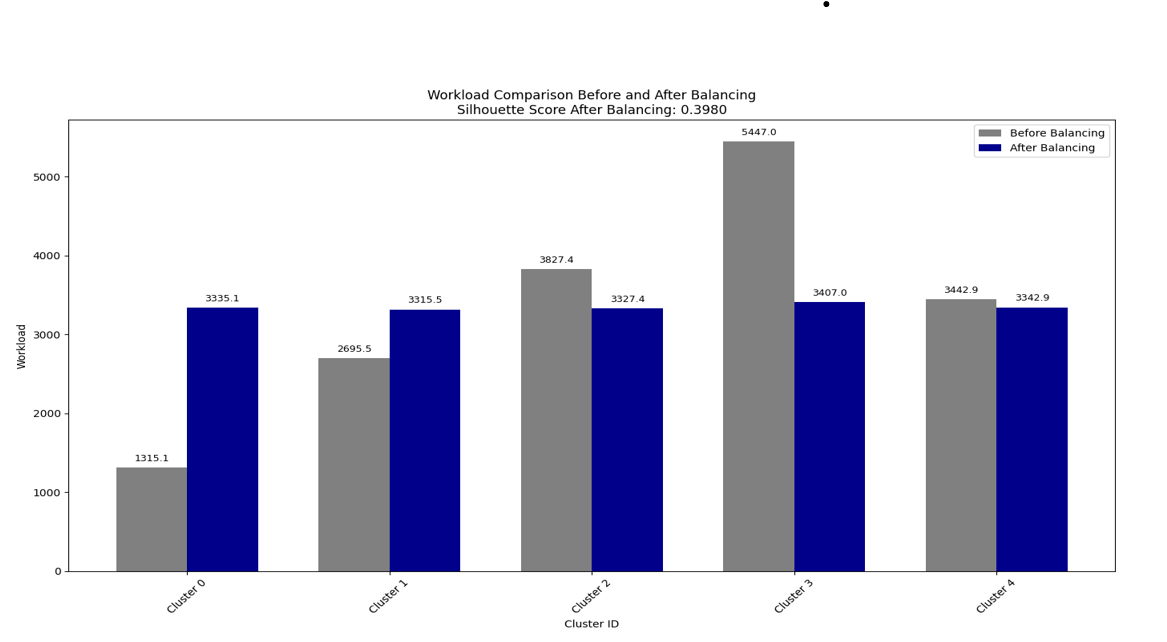
\includegraphics[width=0.85\textwidth]{images/results_hybrid1.png}
        \caption{Hybrid Approach-1: Workload Distribution across Clusters}
        \label{fig:hybrid1_workload}
    \end{figure}
    
    \begin{figure}[H]
        \centering
        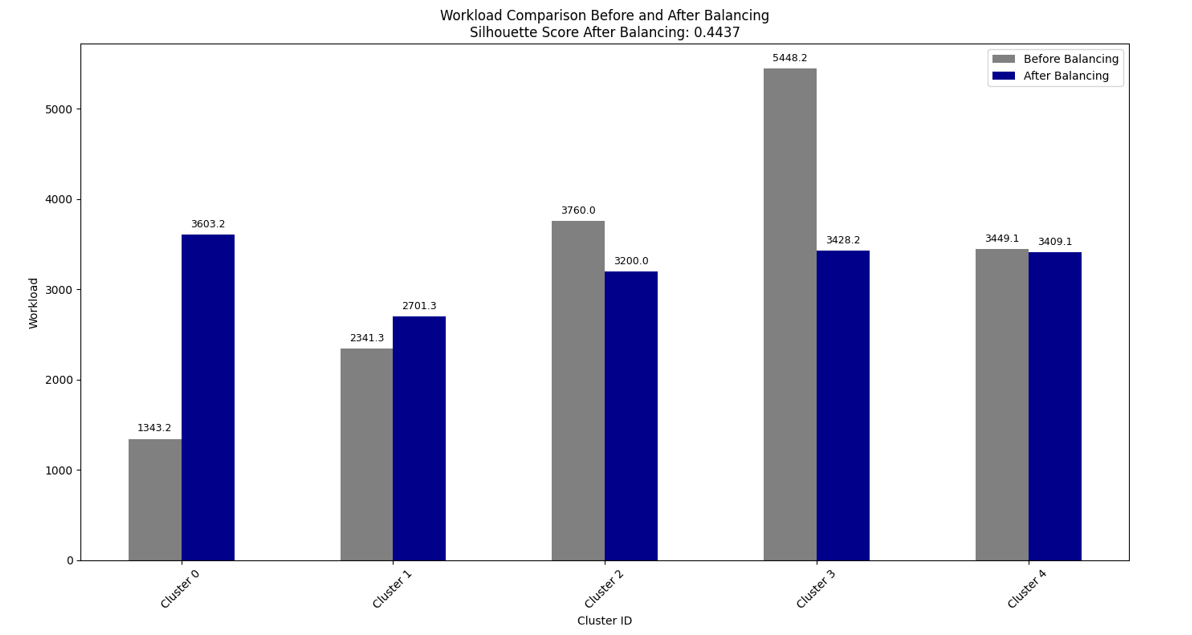
\includegraphics[width=0.85\textwidth]{images/results_hybrid2.png}
        \caption{Hybrid Approach-2: Workload Distribution across Clusters}
        \label{fig:hybrid2_workload}
    \end{figure}

% From the results in Table~\ref{tab:silhouette_scores}, it can be observed that the Hybrid Approach-2 outperformed all other clustering algorithms, achieving the highest silhouette score of 0.5044 for Distributor 1 and 0.4437 for Distributor 7. This indicates that the clusters formed using this approach were more cohesive and well-separated compared to those formed by the other algorithms.
% Moreover, it finds a good balance between workload distribution and geographic proximity. For example, for distributor ID 7, there's a little variance in the clusters being formed however, it has the highest silhouette score as geographical proximity has been set as the priority.
From the results in Table~\ref{tab:silhouette_scores}, it can be observed that the Hybrid Approach-2 outperformed all other clustering algorithms, achieving the highest silhouette score of 0.5044 for Distributor 1 and 0.4437 for Distributor 7. This indicates that the clusters formed using this approach were more cohesive and well-separated compared to those formed by the other algorithms.

Figures~\ref{fig:hybrid1_workload} and~\ref{fig:hybrid2_workload} present a visual comparison of workload distribution across clusters for the two hybrid approaches. While Hybrid Approach-1 shows a slightly more uniform distribution of workload, we ultimately prefer Hybrid Approach-2. The reason is that, despite the marginally greater variance in workload, it achieves significantly better geographical compactness—an important factor reflected in the higher silhouette scores. Prioritizing geographic proximity helps ensure route optimization and operational feasibility, which outweighs the minor imbalance in workload.


\subsubsection{Phase 2 and 3: Scheduling and Route Optimization}
A series of experiments were conducted across different distributors with varying numbers of stores and orderbookers. The following distributors were involved in the experiments:
\begin{table}[h!]
\centering
\begin{tabular}{|c|c|c|}
\hline
\textbf{Distributor ID} & \textbf{Number of Stores} & \textbf{Number of Orderbookers} \\
\hline
1 & 395 & 2 \\
6 & 426 & 4 \\
7 & 580 & 5 \\
131 & 42 & 1 \\
\hline
\end{tabular}
\caption{Distributors and their Assigned Stores and Orderbookers}
\end{table}

The purpose of the experiments was to determine the best combinations of scheduling and route optimization algorithms for each distributor. The experiments were designed to evaluate the performance of different algorithmic combinations in terms of distance and travel time minimization.
This was done by analyzing the total distance and the total traveltime minimized across all orderbookers (results show average of all distributors), and the stores serviced distribution per orderbooker for each day.

\begin{figure}[H]
    \centering
    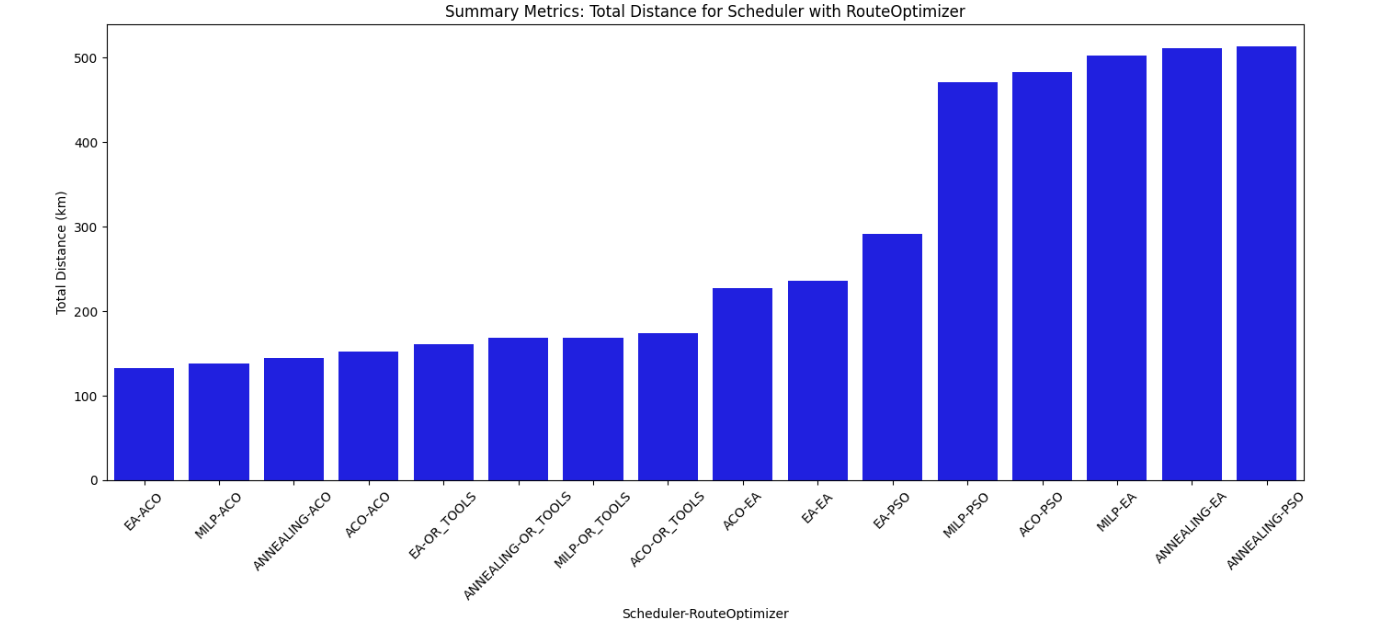
\includegraphics[width=0.95\textwidth]{images/results_distance_all_dis}
    \caption{Total distance for all distributors compared over different combinations.}
    \label{fig:results_distance_all_dis}
\end{figure}

\begin{figure}[H]
    \centering
    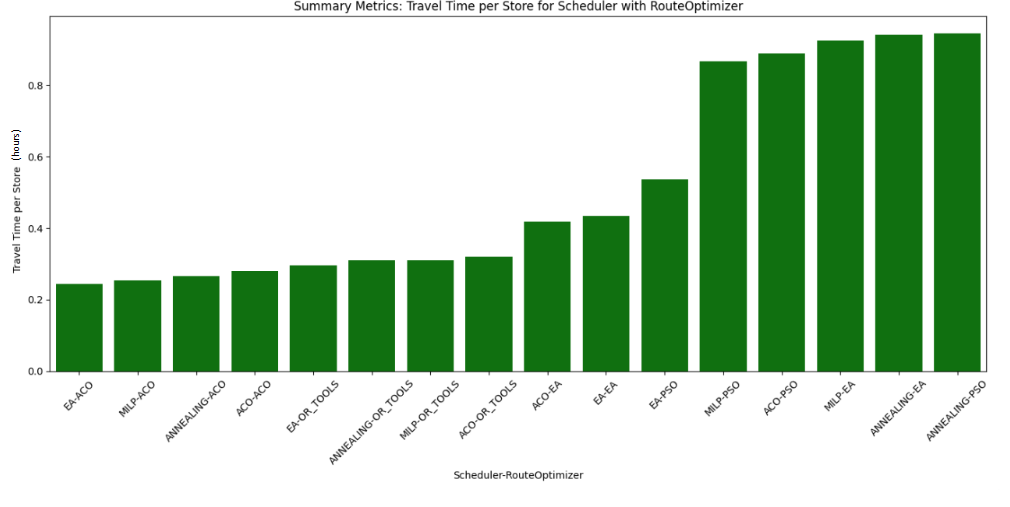
\includegraphics[width=0.95\textwidth]{images/results_time_all_dis}
    \caption{Total time for all distributors compared over different combinations.}
    \label{fig:results_time_all_dis}
\end{figure}

The results in Figure~\ref{fig:results_distance_all_dis} and Figure~\ref{fig:results_time_all_dis} show that one of the top-performing scheduler-route optimizer combinations was EA-OR Tools, which demonstrated strong results in minimizing both travel distance and time, by traveling 
to as less as 150 km in 0.2 hours, as compared to almost 500 kms and 1 hour for the worst combination. OR Tools consistently ranked among the top-performing route optimizers across multiple test cases, whereas the least optimal performance was showed EA nad PSO route optimizers, 
and MILP and simulated annealing schedulers.


% \subsection{Phase 2 and 3: Experiment Results}
% The experiments were conducted by combining different scheduling algorithms with different route optimization algorithms. The findings of each graph is summarized below.



The best performing scheduler-route optimizer combinations for each distributor are as follows:

\begin{table}[H]
    \centering
    \renewcommand{\arraystretch}{1.3}
    \caption{Best Performing Scheduler-Route Optimizer Combinations by Distributor}
    \begin{tabular}{|>{\centering\arraybackslash}p{4cm}@{\hskip 0.5cm}|>{\centering\arraybackslash}p{5cm}@{\hskip 0.5cm}|>{\centering\arraybackslash}p{5cm}|}
    \hline
    \textbf{Distributor} & \textbf{Best Distance Minimized Scheduler-Route Optimizer} & \textbf{Best Travel Time Minimized Scheduler-Route Optimizer} \\
    \hline
    Distributor 7 & EA-OR-Tools & EA-OR-Tools \\
    Distributor 6 & EA-OR-Tools & EA-OR-Tools \\
    Distributor 1 & EA-OR-Tools & EA-OR-Tools \\
    Distributor 131 & EA-ACO & EA-ACO \\
    \hline
    \end{tabular}
    \label{tab:best_schedulers}
\end{table}


    
\section{Results Comparison: Salesflo PJP vs Rahguzar PJP}

This section presents a comparative analysis of Rahguzar's performance against Salesflo's pre-existing PJP plans across three real-world test distributors. Each distributor varied in terms of store count, OB allocation, and planning duration, allowing for a diverse evaluation of route efficiency, time optimization, and system scalability. Metrics analyzed include total distance traveled and total route time under the same operational constraints for both systems.
\subsection{Test Distributors – Summary of Inputs}

To evaluate Rahguzar’s performance and scalability, tests were conducted on three distributors of varying sizes and complexities. Each test case involved a different number of stores, order bookers (OBs), and planning days. The details are summarized below:

\begin{table}[H]
\centering
\caption{Distributor Test Case Overview}
\renewcommand{\arraystretch}{1.3}
\begin{tabular}{|>{\centering\arraybackslash}p{4cm}@{\hskip 0.5cm}|>{\centering\arraybackslash}p{3.2cm}@{\hskip 0.5cm}|>{\centering\arraybackslash}p{3.2cm}@{\hskip 0.5cm}|>{\centering\arraybackslash}p{3.2cm}|}
\hline
\textbf{Distributor} & \textbf{Total Stores} & \textbf{Order Bookers} & \textbf{Plan Duration (days)} \\
\hline
Distributor 1 & 365 & 2 & 3 \\
Distributor 2 & 1153 & 3 & 6 \\
Distributor 3 & 659 & 2 & 6 \\
\hline
\end{tabular}
\label{tab:distributor_summary}
\end{table}

This table provides a consolidated view of the test setups used to benchmark Rahguzar’s planning pipeline across small, medium, and large distributor profiles.

% \subsection{Test Distributor 1 – Results Comparison}

% To evaluate Rahguzar’s performance, the first distributor involved 365 stores serviced by 2 Order Bookers (OBs) over a 3-day plan. The results are summarized below:

% \begin{table}[H]
% \centering
% \caption{Performance Comparison – Test Distributor 1}
% \renewcommand{\arraystretch}{1.3}
% \begin{tabular}{|>{\centering\arraybackslash}p{4cm}@{\hskip 0.5cm}|>{\centering\arraybackslash}p{3.2cm}@{\hskip 0.5cm}|>{\centering\arraybackslash}p{3.2cm}|}
% \hline
% \textbf{Metric} & \textbf{Salesflo} & \textbf{Rahguzar} \\
% \hline
% Total Shops & 365 & 365 \\
% Order Bookers & 2 & 2 \\
% Plan Duration (days) & 3 & 3 \\
% Total Distance (km) & 227.87 & 218.77 \\
% Total Time (hrs) & 35.53 & 35.39 \\
% \hline
% \end{tabular}
% \label{tab:dist1_comparison}
% \end{table}

% Rahguzar reduced the total travel distance by \textbf{9.1 km} and total time by \textbf{0.14 hours}, reflecting modest spatial and temporal efficiency.

% \subsection{Test Distributor 2 – Results Comparison}

% The second distributor included 1153 stores and 3 OBs over a 6-day schedule:

% \begin{table}[H]
% \centering
% \caption{Performance Comparison – Test Distributor 2}
% \renewcommand{\arraystretch}{1.3}
% \begin{tabular}{|>{\centering\arraybackslash}p{4cm}@{\hskip 0.5cm}|>{\centering\arraybackslash}p{3.2cm}@{\hskip 0.5cm}|>{\centering\arraybackslash}p{3.2cm}|}
% \hline
% \textbf{Metric} & \textbf{Salesflo} & \textbf{Rahguzar} \\
% \hline
% Total Shops & 1153 & 1153 \\
% Order Bookers & 3 & 3 \\
% Plan Duration (days) & 6 & 6 \\
% Total Distance (km) & 929.25 & 545.01 \\
% Total Time (hrs) & 113.77 & 108.54 \\
% \hline
% \end{tabular}
% \label{tab:dist2_comparison}
% \end{table}

% Rahguzar achieved a reduction of \textbf{384.24 km} in distance and \textbf{5.23 hours} in time, demonstrating high scalability and optimization capability.

% \subsection{Test Distributor 3 – Results Comparison}

% This case involved 659 stores and 2 OBs, also over a 6-day cycle:

% \begin{table}[H]
% \centering
% \caption{Performance Comparison – Test Distributor 3}
% \renewcommand{\arraystretch}{1.3}
% \begin{tabular}{|>{\centering\arraybackslash}p{4cm}@{\hskip 0.5cm}|>{\centering\arraybackslash}p{3.2cm}@{\hskip 0.5cm}|>{\centering\arraybackslash}p{3.2cm}|}
% \hline
% \textbf{Metric} & \textbf{Salesflo} & \textbf{Rahguzar} \\
% \hline
% Total Shops & 659 & 659 \\
% Order Bookers & 2 & 2 \\
% Plan Duration (days) & 6 & 6 \\
% Total Distance (km) & 143.66 & 142.46 \\
% Total Time (hrs) & 58.95 & 58.99 \\
% \hline
% \end{tabular}
% \label{tab:dist3_comparison}
% \end{table}

% Rahguzar reduced the distance by \textbf{1.2 km}, with a slight increase in time of \textbf{0.04 hours}, indicating comparable efficiency.

\subsection{Summary Across All Distributors}

To illustrate overall performance across all scenarios:

\begin{table}[H]
\centering
\caption{Combined Performance Summary}
\renewcommand{\arraystretch}{1.3}
\begin{tabular}{|>{\centering\arraybackslash}p{2cm}@{\hskip 0.4cm}|>{\centering\arraybackslash}p{3.4cm}@{\hskip 0.4cm}|>{\centering\arraybackslash}p{4cm}@{\hskip 0.4cm}|>{\centering\arraybackslash}p{3.2cm}|}
\hline
\textbf{Distributor} & \textbf{Platform} & \textbf{Total Distance (km)} & \textbf{Total Time (hrs)} \\
\hline
1 & Salesflo & 227.87 & 35.53 \\
  & Rahguzar & 218.77 & 35.39 \\
\hline
2 & Salesflo & 929.25 & 113.77 \\
  & Rahguzar & 545.01 & 108.54 \\
\hline
3 & Salesflo & 143.66 & 58.95 \\
  & Rahguzar & 142.46 & 58.99 \\
\hline
\end{tabular}
\label{tab:combined_summary}
\end{table}

Across all test cases, Rahguzar reduced the cumulative travel distance by \textbf{540.79 km} and time by \textbf{5.41 hours}, validating its effectiveness in optimizing field operations.

\begin{figure}[H]
    \centering
    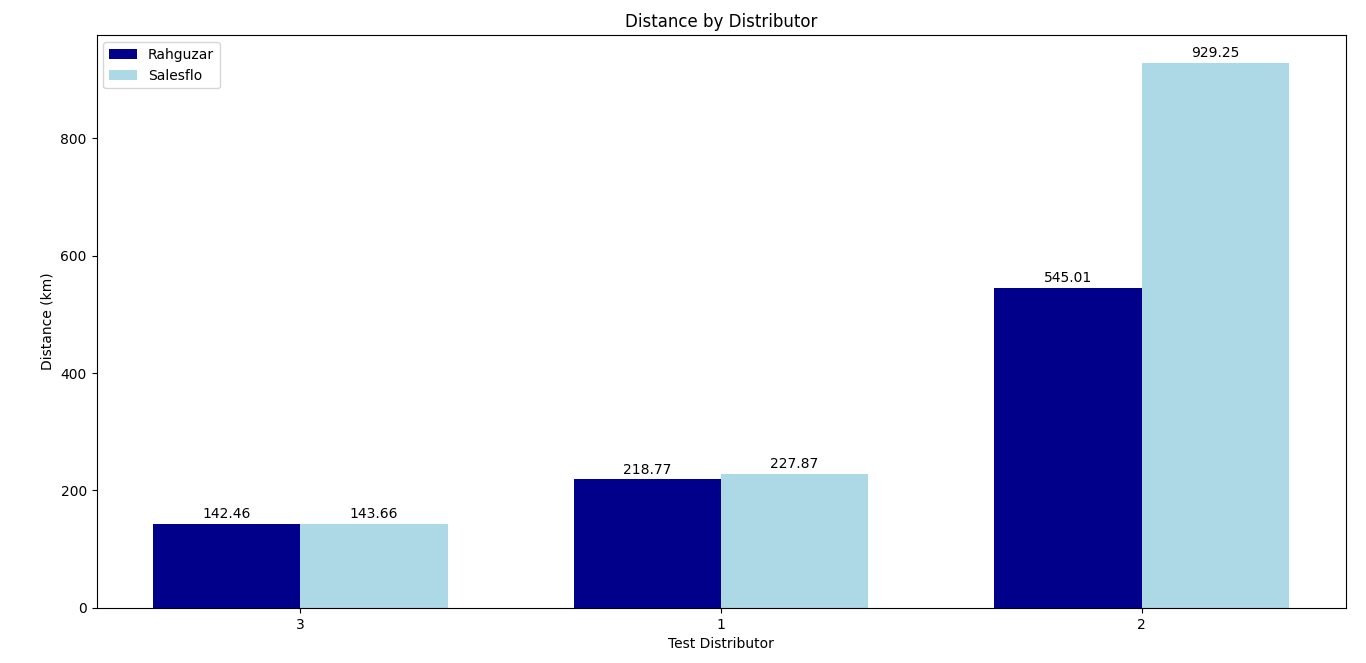
\includegraphics[width=0.95\textwidth]{images/distance_rahgyzar_salesflo_comp}
    \caption{Total distance comparision for the test distributors.}
    \label{fig:results_distance_comparision}
\end{figure}


\begin{figure}[H]
    \centering
    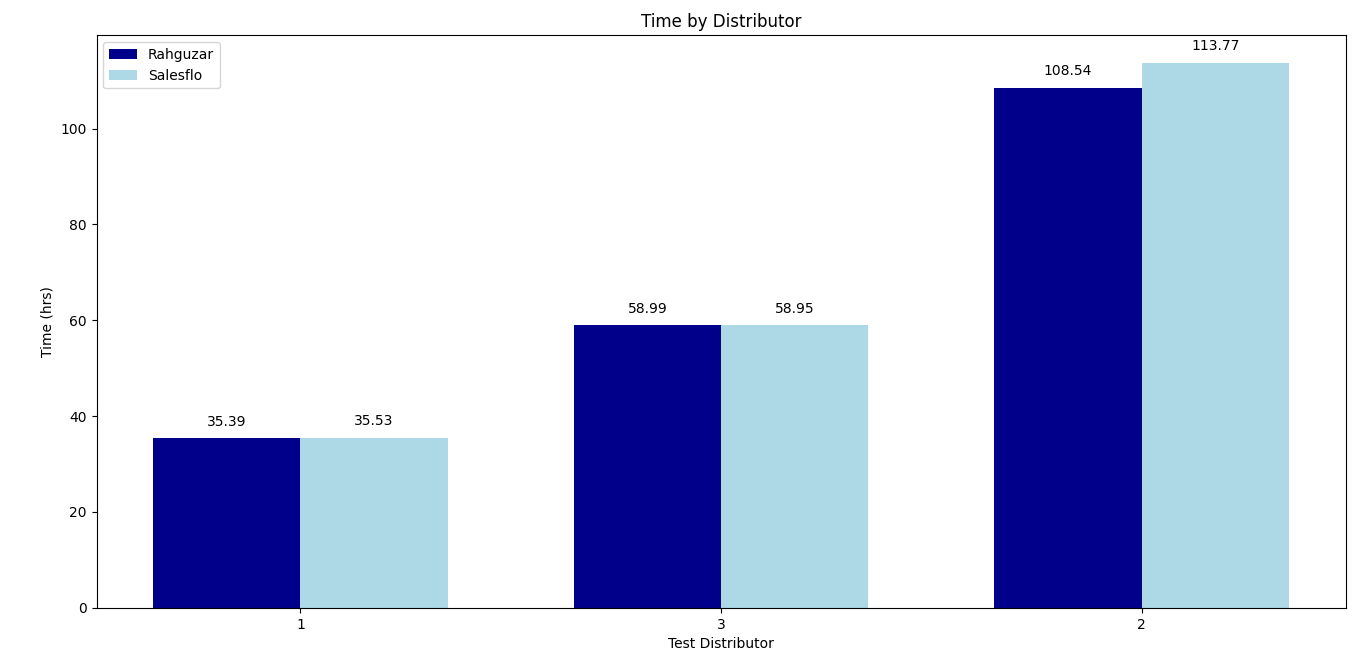
\includegraphics[width=0.95\textwidth]{images/time_rahgyzar_salesflo_comp}
    \caption{Total time comparision for the test distributors}
    \label{fig:results_time_comparision}
\end{figure}


Based on the results of the experiments, the Evolutionary Algorithm (EA) consistently demonstrated strong performance in the scheduling phase, effectively balancing workloads and meeting visit constraints across varying distributor profiles. For route optimization, Google OR-Tools emerged as the most robust and scalable solution, outperforming other algorithms—including ACO and PSO—particularly in large-scale and constraint-heavy scenarios.

The combination of EA for scheduling and OR-Tools for routing provided the most efficient and adaptable pipeline, delivering optimal results in both distance and time minimization. This pairing proved especially effective in consistently handling real-world distributor datasets.

Furthermore, when benchmarked against Salesflo, Rahguzar showed clear improvements in planning efficiency, with notable reductions in total distance traveled and route time. These findings highlight Rahguzar’s potential as a scalable and intelligent planning system that can adapt to operational complexity while delivering measurable gains in field performance.


\chapter{Conclusion and Future Work}
\label{chap:outro}
The Rahguzar project was conceptualized and developed in response to the growing operational challenges faced in manual PJP planning. Through a modular, heuristic-driven methodology combining clustering, scheduling, and routing optimizations, Rahguzar demonstrated substantial improvements in route efficiency, workload distribution, and scalability. The following sections summarize the project’s key outcomes, identify its limitations, and propose directions for future research and system enhancements to further advance intelligent journey planning.

\section{Conclusion}
In this project, we presented Rahguzar, a comprehensive solution for optimizing Permanent Journey Plan (PJP) scheduling in the Fast-Moving Consumer Goods (FMCG) industry. Our system integrates customer clustering, schedule generation via Evolutionary Algorithms, and route optimization using OR-Tools, delivering a robust end-to-end pipeline for sales team planning and management.

Through the integration of real-world datasets and a user-friendly web-based interface, Rahguzar enables dynamic and efficient route planning, helping sales managers minimize travel costs while maximizing coverage and visit compliance. Performance evaluations demonstrate the system’s ability to produce realistic, optimized schedules with significantly improved route efficiency compared to manually designed plans.

The modular architecture allows easy adaptation to various geographical scales, constraints, and business-specific requirements. Moreover, our backend pipeline has been successfully deployed and integrated with a React-based frontend, creating a seamless experience for end users.
\section{Future Work}
In future iterations of Rahguzar, several enhancements can be explored to improve its effectiveness and integration with real-world FMCG workflows. One key direction is the incorporation of real-time traffic data and dynamic scheduling capabilities, enabling the system to adapt routes on the fly in response to disruptions such as delays or cancellations. Integration with Salesflo’s existing mobile platform—which is already widely used by field agents—can also be explored to enable seamless access to route plans, check-ins, and live updates. This would allow on-ground activities to be synchronized with the backend optimization engine, enhancing both usability and data flow. Another promising direction is the use of historical and real-time sales data to drive scheduling decisions. By aligning visit frequency and prioritization with customer-specific sales performance, seasonal trends, and product movement, Rahguzar can help optimize not only travel efficiency but also commercial outcomes. Together, these enhancements can transform Rahguzar into a fully adaptive, data-driven system for sales force automation.

\chapter{Reflections}
\label{chap:reflections}
The Rahguzar project presented an opportunity not only to apply theoretical concepts in a practical setting but also to experience the real-world challenges of system development, collaboration, and research-driven problem solving. This section provides a comprehensive reflection on individual contributions, team dynamics, and process evolution throughout the project lifecycle. By analyzing the gap between initial plans and actual achievements, we aim to capture the key lessons learned and areas for personal and collective growth.

\section{Individual Reflections}

\begin{itemize}
    \item \textbf{Nabila Zahra}: Working on Rahguzar has been one of the most rewarding experiences of my academic life, helping me grow both technically and personally. It was the first time I contributed to a project of this scale, developed in close collaboration with an industry partner—SalesFlo—where every component, from algorithm design to deployment, had real-world implications. This made the journey both challenging and rewarding.

    One of the most meaningful parts of the project for me was working on the scheduling system using an Evolutionary Algorithm. I had previously studied EAs in my Computational Intelligence course at Habib University, but this project allowed me to apply that theoretical knowledge in a much more complex and realistic setting. Translating business constraints into fitness functions, tuning parameters based on performance, and integrating the scheduler into a broader optimization pipeline helped me understand the practical challenges of implementing heuristic algorithms. It reinforced that academic understanding is only the starting point—real-world systems require adaptability, debugging, and iteration beyond what textbooks teach.
    
    Beyond the algorithm itself, I worked extensively on both the backend and frontend of our application. I developed APIs to serve the optimized schedules and routing data, and helped integrate them with our interactive map interface. Seeing the UI reflect our algorithmic output in real time was incredibly satisfying—it reminded me why I enjoy building end-to-end systems.
    
    I also stepped out of my comfort zone by handling deployment tasks. I learned how to use Docker to containerize OSRM, and how to set up and configure AWS EC2 and RDS with PostgreSQL. These were tools I had not worked with before, and figuring them out taught me how to be resourceful and persistent when dealing with unfamiliar systems. At times, debugging deployment issues felt frustrating, but I now see how those moments pushed me to grow the most.
    
    What stood out to me throughout this project was how much value lies in cross-functional thinking—understanding how the backend affects the frontend, how the database interacts with APIs, and how deployment choices affect performance. Working on Rahguzar helped me connect these dots and become more confident in navigating complex, integrated systems.
    
    Most importantly, this project reminded me that challenges are learning curves. Whether it was refining the EA scheduler, troubleshooting server errors, or adapting designs based on feedback, each obstacle became an opportunity to learn, grow, and build something better. I walk away from this project with a deeper appreciation for teamwork, a stronger technical foundation, and a clearer vision of the kind of systems I want to build in the future.

    \item \textbf{Iqra Azfar}: Over the duration of the project, I was not only dedicated to doing extensive research and examining different facets of the issue, but also to developing essential technical and soft skills on an ongoing basis. The methodology included picking up new tools, studying intricate concepts, and implementing them to solve real-world problems. Collaboration with my team members was an enriching experience, where I actively participated in brainstorming meetings, solution creation, and decision-making. Working with others showed me the value of effective communication, flexibility, and respect towards one another, particularly in dealing with conflicts or differing opinions. These experiences helped me learn more about teamwork, problem-solving, and lifelong learning.
    \item \textbf{Muhammad Youshay}: Embarking on this project was an enriching experience, particularly due to the opportunity to solve an actual industry problem presented by SalesFlo in the FMCG sector—a field entirely new to me. This required a deep understanding of the intricacies involved in permanent journey plan (PJP) scheduling, pushing me to thoroughly analyze operational constraints, optimization criteria, and stakeholder needs. The Human-Centered Design (HCD) approach was central to our methodology, enabling us to systematically empathize with end-users, define core problems, ideate viable solutions, prototype concepts, and iterate based on real-world feedback.

    The experience significantly expanded my skill set. Leveraging my academic knowledge from Habib University's courses, particularly Computational Intelligence, was crucial in developing the evolutionary algorithm component of our project. This course provided the theoretical foundation and practical techniques that enabled the design and fine-tuning of our hybrid optimization approach, effectively addressing complex, multi-objective problems. Additionally, my problem-solving abilities and logic-building skills greatly improved as I navigated challenges such as workload balancing, geographic clustering, and routing optimization. Exploring the problem from different perspectives and applying diverse analytical lenses was particularly enlightening.
    
    From a technical standpoint, I enhanced my proficiency in Python, OR-Tools, and data preprocessing techniques. Furthermore, interacting extensively with PostgreSQL and cloud-based systems like AWS strengthened my database management and backend development capabilities, preparing me for more complex technical tasks in the future.
    
    Working in a team presented both enriching experiences and notable challenges. Our team brought together individuals with different ideas, approaches, and technical expertise. Achieving consensus required effective communication, open-mindedness, and patience. Navigating through varied perspectives and integrating everyone's inputs to form cohesive solutions taught me invaluable lessons in teamwork, collaboration, and leadership.
    
    Overall, the experience was immensely rewarding, significantly boosting both my technical expertise and soft skills. I have emerged more confident in my ability to approach complex real-world problems with structured, innovative solutions, and equipped to thrive in collaborative environments.
    \item \textbf{Rabia Shahab}: Working on Rahguzar has been one of the most impactful experiences of my undergraduate journey, offering a chance to apply technical skills to a meaningful real-world problem. Collaborating with SalesFlo introduced a level of complexity and accountability that shaped how we approached both design and implementation. Our work wasn't just theoretical—it had to make sense in a business context and stand up to practical constraints, which made the learning curve steep but highly rewarding.

    My core contributions focused on the areas of developing the Evolutionary Algorithm (EA) scheduler and designing a performance dashboard. The EA scheduler pushed me to move beyond textbook models and think critically about how to encode real-world business requirements—such as fairness in visit distribution and route efficiency—into algorithmic logic. Balancing multiple objectives, tuning parameters, and debugging unexpected behaviors taught me that optimization in real systems is messy, and that iteration is essential.
    
    Simultaneously, building the dashboard gave me a deeper appreciation for data interpretation and user-centered design. It helped me identify and prioritize the KPIs that actually matter—things like distance coverage, visit gaps, and time allocation per resource. Creating a clear interface to display these metrics not only made the system more usable, but also helped bridge the communication gap between the technical team and non-technical stakeholders and enable them to be more data-driven. It was a reminder that even the best algorithm needs to be transparent and interpretable to deliver real value.
    
    Throughout the project, I also explored new technical tools that were initially unfamiliar. I worked with OSRM to integrate routing functionality and used Docker to containerize services for a smoother deployment process. These experiences gave me hands-on exposure to backend infrastructure and helped me understand how different system components—schedulers, route engines, data pipelines—must work together in sync.
    
    Equally important was the experience of working with my teammates. We each brought different strengths to the table, and there were moments where progress felt uncertain—whether due to technical issues or conflicting ideas. However, through open discussion, shared debugging sessions, and brainstorming under pressure, we consistently found ways forward. I learned that collaboration isn't just about dividing tasks—it's about supporting each other, challenging assumptions, and finding common ground when faced with complexity.
    
    Rahguzar taught me that building real systems requires not just technical skills but also adaptability, empathy, and trust in your team. I leave this project with greater confidence in my ability to contribute to large, interdisciplinary efforts, and a stronger sense of the kind of systems and teams I want to be a part of in the future.
    
\end{itemize}

\section{Team Reflection}
% Collaboration experience, role distribution, communication, and teamwork challenges.
Working together on Rahguzar was a deeply collaborative experience that taught us the value of shared vision, consistent communication, and mutual accountability.
While we were united by a shared goal, the process of getting there involved navigating a variety of challenges that tested our coordination, communication, and adaptability. One of the most significant challenges we encountered was working at different paces. Each team member had their own academic and personal commitments, and synchronizing our work schedules proved difficult at times. There were also disagreements on how to approach certain parts of the problem, particularly in algorithm design, interface behavior, and system architecture.
At one point, we struggled to align our approaches to problem-solving, particularly in how to structure the optimization logic, divide backend responsibilities, and sequence integration with the frontend. Each of us had different interpretations of the problem and varying ideas on how best to implement certain features. These disagreements sometimes led to delays and overlapping efforts. However, they also turned out to be important learning opportunities. What helped us move forward was our ability to step back, have honest discussions, and actively listen to one another. The guidance and support we received from our supervisor and mentors during these phases were especially valuable. Their input helped us untangle complex decisions, identify a shared direction, and turn moments of friction into productive design conversations.
Despite the differences in working styles and technical opinions, we learned to trust each other’s strengths and make space for every perspective. As the project progressed, we grew more coordinated and developed a rhythm that allowed us to work more effectively together. Ultimately,Rahguzar was not just a technical achievement, but a product of collective resilience, trust, and shared commitment to solving a real-world problem together.
\section{Process Reflection}
% What worked well? What could be improved in the your project?
Looking back at the process, one of the things that worked particularly well was our decision to follow an iterative and research-driven development approach. Early in the project, we focused on understanding the problem deeply through industry interviews, literature review, and small-scale experiments. This helped us avoid jumping prematurely into implementation and instead guided our design with clarity and purpose.
Another strength was our consistent engagement with real-world data and constraints. By validating our design choices against actual operational needs provided by SalesFlo, we ensured that our solution stayed grounded and practical.

However, we also faced challenges that impacted our efficiency. A major bottleneck occurred when all of us were working on different parts of the codebase simultaneously. While this parallel effort helped accelerate feature development, it made integration complex and time-consuming. Merging work from multiple branches while ensuring compatibility and system stability required multiple debugging sessions and technical compromises. In hindsight, a more modular and version-controlled integration plan from the start could have reduced friction.

We also underestimated the time needed for certain tasks, particularly data integration and testing. Delays in data availability affected our ability to validate early outputs, and unexpected inconsistencies in the dataset required additional preprocessing.

Despite these challenges, the process evolved and improved over time. We became more deliberate in dividing tasks, more consistent in communication, and more disciplined in tracking progress. This experience highlighted the importance of not just technical knowledge, but also process design and team coordination in building real-world systems.

% \section{Plan vs Achievment}
% What was proposed vs what was achieved? 
% Were any proposed features removed/were any features added that were not proposed initially? 
% What are the reasons for these choices? 
% What are opportunities and challenges led to these design decisions? 
% In the initial stages of development and testing, the project encountered several challenges, particularly in the selection and evaluation of appropriate algorithms. One of the key difficulties arose from operational constraints provided by SalesFlo, including specific scheduling rules based on store types. For example, wholesale stores required a minimum gap of two days between consecutive visits. These requirements introduced additional complexity into the scheduling logic that was not fully anticipated during the planning phase.

% The original design included the use of the Google Maps API for generating distance matrices essential for route optimization. However, during implementation, we faced quota limitations and cost-related constraints that made it unsustainable for repeated large-scale use. As a result, we migrated to the Open Source Routing Machine (OSRM), which offered a cost-effective and reliable alternative. OSRM integrated smoothly with the backend system and allowed us to maintain routing functionality without dependency on third-party paid services.

% Additionally, the performance metrics defined at the start of the project were revised. Initially, we focused on general algorithm efficiency. As the project progressed, these metrics were refined to better reflect the quality of the generated Permanent Journey Plans (PJPs). New evaluation criteria included factors such as adherence to visit frequency requirements, practical feasibility of routes, and overall balance in daily assignments. These changes were informed by observations during pilot testing and helped ensure that system outputs aligned more closely with operational expectations.

% Another major change involved the dashboard technology. The initial plan was to use Power BI for data visualization. However, Power BI presented limitations in terms of scalability, customization, and backend integration. To address this, we transitioned to a custom-built solution using React for the frontend and Flask for the backend. This provided improved control over interface design and enabled real-time communication with the core system. During this process, an additional feature was also introduced: the ability to generate journey plans for extended planning windows while still meeting the original constraints—such as visit frequency, rest-day intervals, and fair workload distribution across order bookers.

% These design changes reflect an adaptive and iterative approach guided by technical constraints and practical deployment considerations. While some originally proposed features were modified or replaced, new capabilities were added to enhance system performance and usability. Overall, the project evolved in a way that better aligned with both user requirements and system scalability, resulting in a more robust and deployment-ready solution

\section{Plan vs Achievement}


The initial vision for the Rahguzar system was shaped by academic research, stakeholder discussions, and a focus on building a modular, data-driven solution for journey plan optimization. While the core objectives remained consistent throughout the project, many aspects of the system evolved significantly during development. These changes were driven by technical constraints, real-world deployment challenges, and feedback from pilot testing. As a result, several design decisions were revised, new features were added, and some proposed components were removed—ultimately leading to a more practical, efficient, and scalable system.
\\
\textbf{Algorithm Design:} Initially, a basic heuristic-based approach was proposed for assigning stores to days and order bookers. However, this proved insufficient to meet complex requirements such as visit frequency enforcement, workload balancing, and multi-day planning. We pivoted to a custom-built Evolutionary Algorithm (EA), which allowed encoding multiple operational constraints into a single fitness function. This shift enabled more flexible and scalable scheduling under real-world conditions.
\\
\textbf{Routing Engine:} The original system design relied on the Google Maps API for generating travel distances and times. During development, cost limitations and API quotas led us to migrate to a Dockerized, self-hosted instance of the Open Source Routing Machine (OSRM), which offered a scalable, open-source alternative. OSRM integrated seamlessly into our Flask backend and provided accurate routing using OpenStreetMap data, supporting high-performance route sequencing at no additional cost.
\\
\textbf{Technology Stack:} While Power BI was initially considered for dashboard visualization, it lacked the flexibility needed for real-time updates and seamless backend integration. This limitation prompted a shift to a custom React-based dashboard, with Flask serving data endpoints. The result was a more interactive and responsive UI, with tighter control over both the visual and functional layers of the system.
\\
\textbf{Data Management:} Contrary to initial assumptions, store data and geographic metadata required substantial preprocessing. Duplicates, missing coordinates, and inconsistent fields had to be addressed through custom scripts and validation steps. These preprocessing efforts became crucial to maintaining accuracy in clustering, scheduling, and route generation.
\\
\textbf{Integration Strategy:} Our original plan was to integrate all components toward the final phase of development. This approach proved problematic, especially as different modules evolved in parallel. As a result, we adopted a continuous integration model midway through the project, merging backend and frontend functionality incrementally to detect compatibility issues earlier.
\\
\textbf{Performance Metrics:} Initially, success was to be measured in terms of algorithm speed and distance minimization. However, real-world feedback highlighted the need for more meaningful metrics. We revised our KPIs to include visit frequency adherence, shift time compliance, workload standard deviation, and travel vs in-store time ratios. These metrics offered more actionable insights and improved the system’s operational relevance.
\\
\textbf{Feature Additions:}
\begin{itemize}
    \item \textbf{Custom Day Planning:} Instead of fixed weekly or monthly planning cycles, the system now allows users to define custom durations for journey plans, providing greater flexibility.
    \item \textbf{Automatic Extra Day Allocation:} If the number of available days is insufficient to accommodate all required store visits, the system intelligently adds extra working days to complete the plan while maintaining constraint compliance.
    \item \textbf{Dynamic Rerouting and Manual Overrides:} Managers can trigger rerouting in real time by modifying store assignments, improving adaptability.
\end{itemize}

\textbf{Feature Removals:}
\begin{itemize}
    \item \textbf{Sales Data Integration:} Early plans included integration with historical sales data to prioritize high-performing stores. This feature was removed due to unavailability of sales records and limited scope in the pilot phase.
    \item \textbf{Mobile Application Support:} Native mobile deployment was removed from the scope in favor of a responsive web-based interface, reducing complexity while retaining cross-device accessibility.
    \item \textbf{OB Recommendation System:} A proposed OB-store matching suggestion engine was deprioritized due to time constraints and shifting focus toward core scheduling logic.
\end{itemize}

In summary, while several originally proposed features were re-evaluated or removed, new capabilities were introduced that better addressed stakeholder needs and system scalability. These adaptive decisions reflect the project’s iterative development philosophy and contributed to a more robust, usable, and deployment-ready solution.


\begin{appendices}

% \titleformat{\chapter}[hang]{\bf\huge}{Appendix \thechapter.}{2pc}{}
  
% % This appendix is optional.
% \chapter{More Math}
% % Here, we describe the background math for the techniques used in the text.

% % This appendix is required if the data set is not fully described in the main text.
% \chapter{Data}
% Here is a dump of our 2TB data set. Enjoy!

% This appendix is required if the code is not fully described in the main text.
\chapter{Code}
% EITHER dump your code here. No one except HEC likes this.
Here is our code.

% inspired by https://xkcd.com/221/
\begin{lstlisting}[language=python, showstringspaces=false,frame=single]
  print('Hello World!')
  print('Computing true random number.')
  print('Capturing interstellar radiation.')
  print('This will take time!')
  import random
  import time
  time.sleep(3600*random.randint(1,10))
  print(4)
\end{lstlisting}

% OR, link to your GitHub repository. Everyone but HEC will like this.
% Our code can be found at \url{https://github.com/habib-university/Kaavish-Template}.

%%% Local Variables:
%%% mode: latex
%%% TeX-master: "../report"
%%% End:

\end{appendices}


% Print the bibliography with a ToC entry and titled, "References".
\printbibliography[heading=bibintoc,title={References}]

\end{document}

%%% Local Variables:
%%% mode: latex
%%% TeX-master: t
%%% End:
